%!TEX root = ../thesis.tex
%*******************************************************************************
%*********************************** Sixth Chapter *****************************
%*******************************************************************************

\chapter{Results}  %Title of the First Chapter
\label{chapter results}

\ifpdf
\graphicspath{{Chapter6/Figs/Raster/}{Chapter6/Figs/PDF/}{Chapter6/Figs/}}
\else
\graphicspath{{Chapter6/Figs/Vector/}{Chapter6/Figs/}}
\fi

One of the aims of this study was to check how the designed impedance device detects plethysmography signals from one limb. Another objective was to verify how what changes in plethysmography waveform are detectable by the instrument.\nknote{??prev sentences no sense} As described in chapter \ref{chapter design}, the designed device is capable of providing electrical signals comparable to the impedance of the body section. The iPG instrument provides output ports of the current driven into the patient, impedance readings and plethysmography waveform of volume under test. In chapter \ref{chapter procedure}, how to convert these signals from voltage representations into readable units was described, such as impedance values in ohms (\si{\ohm}) and currents (\si{\ampere}). Then, a GUI provided analysis of the signals, as well as post-processing options. Lastly, the data needs to be transformed into equivalent measurements of blood flow.\nknote{first you are talking about what you did then switching to presnet im confused especially as you say lastly making it sound like its a list in order}

As explained in chapter \ref{chapter procedure}, the experiment proceeds by recording five minutes of baseline signal followed by a level of occlusion. Seven different regions are identifiable in the experiment, as presented in Table \ref{tbl:Z_regions}. Additionally, occlusive events are represented as shaded areas in figure \ref{fig:rb:all_participants}. Regions 1, 3, 5 and 7 refer to the five minutes of baseline waveform. On the other hand, regions 2, 4 and 6 are equivalent to venous, partial arterial and total occlusions.

This chapter describes the results obtained from the experimental work for all the physiological measurements received from the study participants with all the instruments. The outcome of the data collected is presented in detailed tables and graphs where the data was converted into its meaningful units. 

There is more detailed work on the results obtained from the impedance device to verify the efficiency of the instrument designed. \nknote{??}Analysis of the impedimetric values will be described as well as it's equivalent measurement in blood flow during baseline and occlusive events. Subsequently, in the next chapter, the results of the impedance device will be compared to the others regarding venous and arterial flow changes.

\mynote{First report the volume measured and the impedance correlated}
\mynote{Add an image of one participant with all the measurements in one place. }

%%********************************** % Section 5.1 ******************************************
\section{Physiological measurements}
\label{section results 1}
At the beginning of the research study, from the participants recruited population characteristics,\nknote{????no sense} physiological measurements and blood pressure values were taken \mynote{reference to section that includes a figure of the arm with the measurements position}. In total, three female and six male participants took part of the study. Their ages ranged between \SIrange{23}{37}{year-old} (mean \num{29.12(494)}). The table \ref{tbl:physiological} overviews the data and measurements collected from the participants prior to the experiment.

\begin{table}[!htbp] %tbl:physiologica
	\caption{Participants' forearm measurements and initial volume.}
	\label{tbl:physiological}
	\centering
	\begin{tabular}{lcc|ccc}
		\toprule
		&              &              &         \multicolumn{3}{c}{\textbf{Dimensions [\si{\cm}]}}         \\
		& \textbf{Age} & \textbf{Sex} & \textbf{Arm length} & \textbf{Shoulder} & \textbf{Total length} \\
		&              &              &                     &  \textbf{to heart}   &                       \\ \midrule
		Participant 1 &      26      &     Male     &         80          &          26          &          106          \\
		Participant 2 &      23      &    Female    &         66          &          24          &          90           \\
		Participant 3 &      27      &    Female    &         74          &          24          &          98           \\
		Participant 4 &      37      &     Male     &         68          &          24          &          92           \\
		Participant 5 &      29      &    Female    &         62          &          24          &          86           \\
		Participant 6 &      36      &     Male     &         70          &          24          &          94           \\
		Participant 7 &      29      &     Male     &         73          &          23          &          96           \\
		Participant 8 &      26      &     Male     &         69          &          23          &          92           \\ \bottomrule
	\end{tabular}
\end{table}

From the sensing electrodes position, it is possible to estimate the segment's volume by measuring the distance between electrodes ($l$), and the circumference of each electrode (C$_1$ and C$_2$).  This measuring method is not very accurate (see section \mynote{Add reference to a section where how measurements were taken}) but at least gauges a picture of the initial volume of the conductive segment. Table \ref{tbl:measurments} shows the dimensions of the participants forearm between the sensing electrodes and the segment's volume calculated from Equation \ref{eq:v_e}.

\begin{table}[!htbp] %tbl:measurments
	\caption{Participants' forearm measurements and initial volume.}
	\label{tbl:measurments}
	\sisetup{separate-uncertainty=true}
	\centering
	\begin{tabular}{lcccccc    S[table-format=2.2]@{\,\( \pm \)\,}S[table-format=1.2]}
		\toprule
		&  \textbf{L [\si{\cm}]}   &  \textbf{C$_1$ [\si{\cm}]}  &  \textbf{C$_2$ [\si{\cm}]}  &   \textbf{Ve [\si{\cubic\cm}]} \\\midrule
		Participant 1 & 14.8 & 17.5 & 27.5 & 606.05 \\
		Participant 2 & 11.0 & 15.0 & 20.0 & 269.90 \\
		Participant 3 & 13.0 & 19.0 & 26.5 & 540.27 \\
		Participant 4 & 10.0 & 17.5 & 25.0 & 363.07 \\
		Participant 5 & 10.0 & 17.5 & 23.5 & 336.81 \\
		Participant 6 & 11.0 & 18.5 & 27.0 & 458.32 \\
		Participant 7 & 13.5 & 15.0 & 23.0 & 393.55 \\
		Participant 8 & 11.5 & 17.0 & 23.5 & 378.49 \\ \bottomrule
	\end{tabular}
\end{table}

Executing a mechanical occlusion of the upper arm limits the blood flow towards the forearm. As detailed in chapter  \ref{chapterprocedure}, a blood pressure was taken before the study began. The mean systolic and diastolic pressures were \SI{116.25(1366)}{\mmHg} and \SI{72.75(723)}{\mmHg} respectively. Venous occlusion took place below systolic pressure (mean \SI{55.00(801)}{\mmHg}), partial arterial pressure calculated from equation \ref{eq:meanpressure} was about  \SI{94.63(1021)}{\mmHg} and total occlusion was around \SI{136.25(1367)}{\mmHg}. Table \ref{tbl:occlusions} details the blood pressures recorded.

\begin{table}[!htbp] %tbl:occlusions
	\caption{Participants' initial blood pressure and levels for venous, partial arterial and total occlusion.}
	\label{tbl:occlusions}
	\centering
	\begin{tabular}    {lcccc}
		\toprule
		& \textbf{Blood pressure}  &  \textbf{Occlusion 1}   & \textbf{Occlusion 2}  &  \textbf{Occlusion 3} \\
		&  [\si{\mmHg}]   &        [\si{\mmHg}]  &    [\si{\mmHg}]   &  [\si{\mmHg}]\\ \midrule
		Participant 1  &  124/78   &        50  &    101   &  144\\ 
		Participant 2  &  105/65   &        50  &     85   &  125 \\
		Participant 3  &  120/78   &        60  &     99   &  140 \\
		Participant 4  &  120/72   &        60  &     96   &  140 \\
		Participant 5  &  100/60   &        40  &     80   &  120 \\
		Participant 6  &  143/82   &        60  &    113   &  163 \\
		Participant 7  &  107/73   &        65  &     90   &  127 \\
		Participant 8  &  111/74   &        55  &     93   &  131 \\\bottomrule
	\end{tabular}
\end{table}


%%********************************** % Section 5.2 ******************************************
\section{Impedance results from mean resistivity value}
\label{section results 2}
As described in the previous chapters\mynote{Maybe add a reference of the past chapter design of the device}, the iPG device provides an output signal denominated $Z_{DC}$ which is equivalent to the mean impedance value of the elbow to wrist section. Moreover, it includes an AC component equal to a low-resolution plethysmography signal. However, this waveform at this point is unwanted, however, it will be helpful for analysis beat by beat. This section will analyse the changes that the impedance baseline suffer \nknote{?suffer not right word}during the different events of the experiment.

The resistivity mean value is known as basal impedance, which is equivalent to value $R_B$ as described by Nyober's equation \ref{eq:Nyober} or the foot of the signal in the plethysmography waveform. In other words, it is the value of the impedance before circulation occurs and is composed of the impedance contribution of bone, muscle, fat, skin and residual blood within the vessels.

\mynote{Maybe add a waveform explaining where the signal was extracted form or from a reference to another section}

As explained in detail in chapter \ref{chapter procedure}, the experimental protocol required \nknote{??}executing a mechanical compression using a cuff to limit venous and arterial blood inflow and outflow. The level of pressures during these occlusions have been recorded in table \ref{tbl:occlusions}. Firstly, venous blockage causes a swelling of the forearm by filling of the capillaries below the blockage. Secondly, during partial arterial occlusion, the incoming arterial flow is restricted causing a slow filling of the forearm's vessels. In both kinds of occlusions, the blood pooling increases the volume of the forearm's segment, hence producing a variation in the baseline signal. In contrast, total occlusion completely eliminates the blood inflow under the obstructed section; it is a tourniquet effect. Thus, the resultant impedance should be similar to the baseline resistivity.

Analysing the baseline necessitates eliminating the waveform component of the signal. In section \mynote{Add a section in data processing explaining how the value of $R_B$ was extracted for this analysis and reference it.} was explained \nknote{was explained?}in detail the steps required to obtained this level of the signal. In the end, only the values from the foot of the signal equivalent to $R_B$ were extracted. \nknote{why?}Figure \ref{fig:rb:all_participants} shows all the basal impedance signals of all the participants during the whole study. As can be seen, some signals were affected by motion artefact. In fact, other instruments such as PPG and Doppler ultrasound also picked up these sort of fluctuations. Table \ref{tbl:Z_regions} shows the mean value of the impedance separated in regions or events. In the following sections, the changes in basal impedance will be analysed in more depth. 

\begin{figure}[!htbp]  %fig:rb:all_participants
	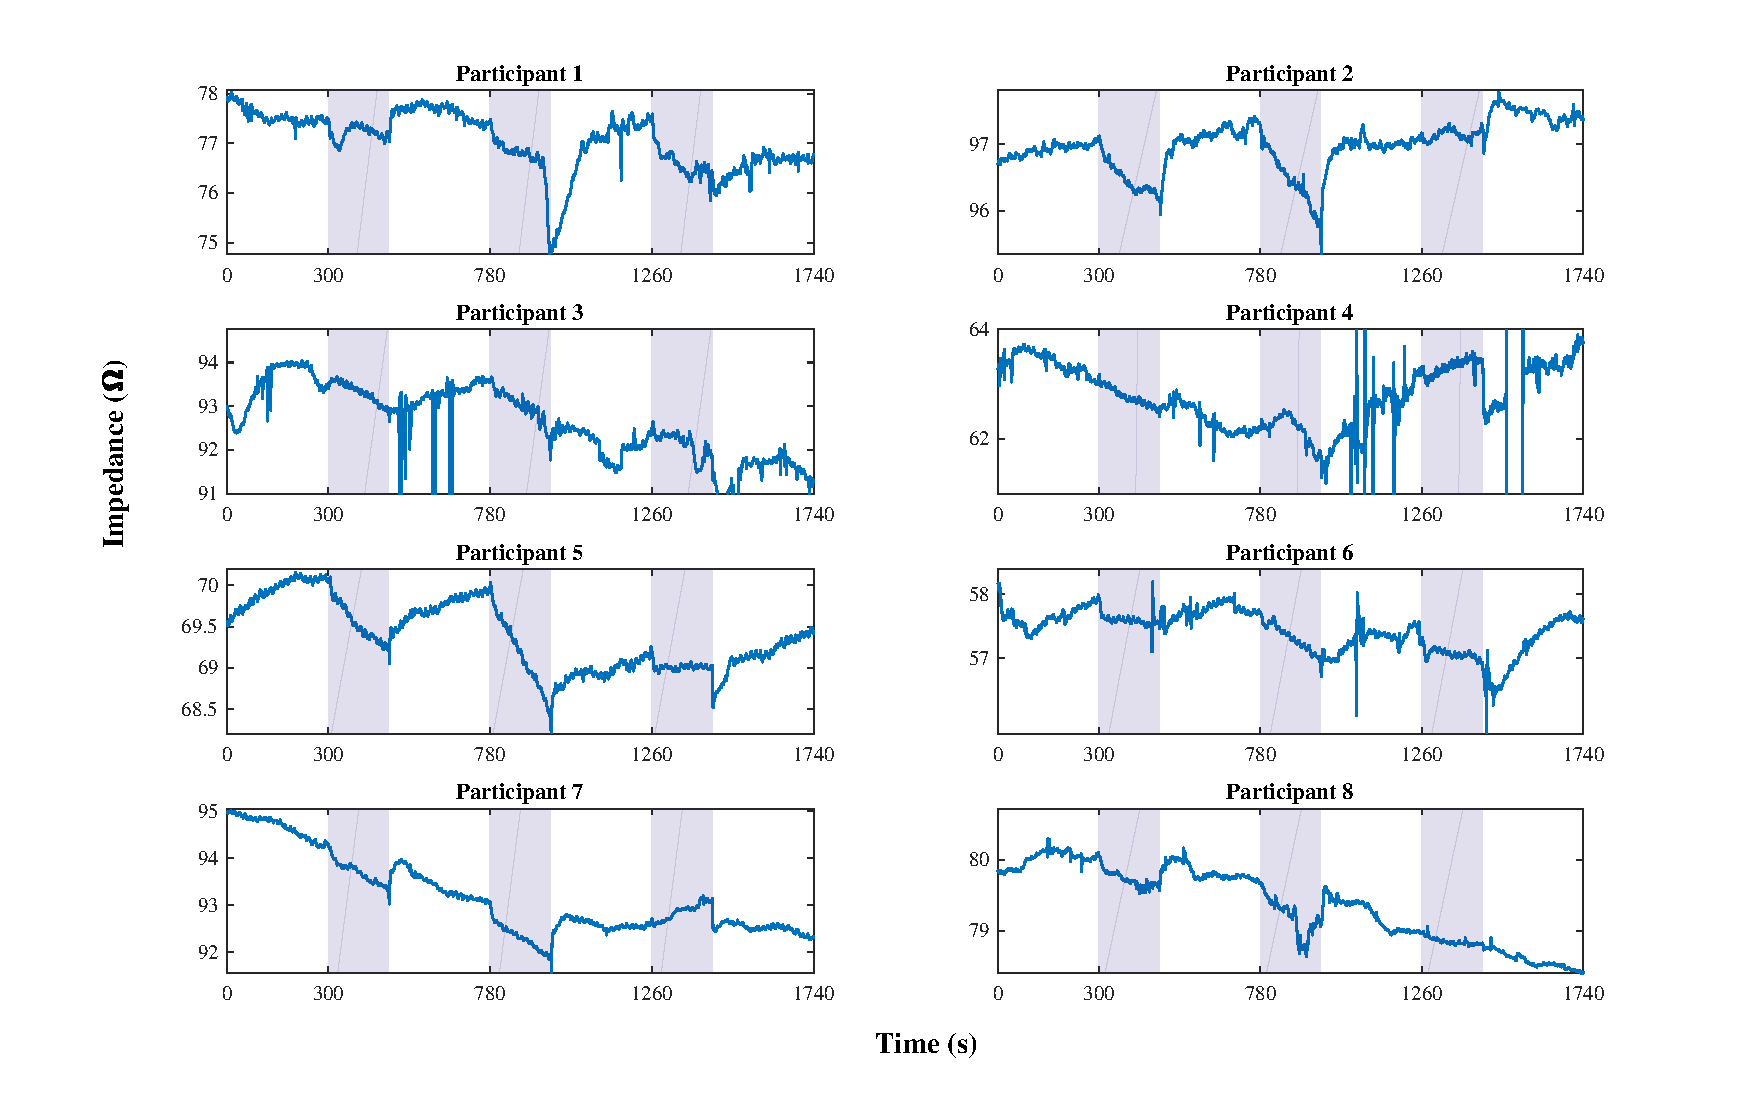
\includegraphics[width=\textwidth,height=\textheight,keepaspectratio]{figure1}    
	\caption[Measurements of the basal impedance during the whole study]{Basal impedance of all the participants during the whole study. The data collected has been divided into regions. The regions (1,3,5 and 7) in white colour represent baseline measurements. The shaded areas (regions 2,4 and 6) represent occlusive events.  }
	\label{fig:rb:all_participants} 
\end{figure}

\begin{sidewaystable}[!htbp] %tbl:Z_regions
	\caption[Mean basal impedance is divided in seven regions]{Mean basal impedance is divided into seven regions according to the time of the event. Measurements include standard deviation from each value. }
	\label{tbl:Z_regions}
	\centering
	\begin{tabular}    {l
			*{7}{S[table-format=2.2]@{\,\( \pm \)\,}S[table-format=1.2]} %Format for Z+-std
		}
		\toprule
		&\multicolumn{2}{c}{\textbf{Region 1}}&\multicolumn{2}{c}{\textbf{Region 2}}&\multicolumn{2}{c}{\textbf{Region 3}}&\multicolumn{2}{c}{\textbf{Region 4}}&\multicolumn{2}{c}{\textbf{Region 5}}&\multicolumn{2}{c}{\textbf{Region 6}}&\multicolumn{2}{c}{\textbf{Region 7}}\\
		&\multicolumn{2}{c}{\small{\SIrange{0}{300}{\second}}}&\multicolumn{2}{c}{\small{\SIrange{300}{480}{\second}}}&\multicolumn{2}{c}{\small{\SIrange{480}{780}{\second}}}&\multicolumn{2}{c}{\small{\SIrange{780}{960}{\second}}}&\multicolumn{2}{c}{\small{\SIrange{960}{1260}{\second}}}&\multicolumn{2}{c}{\small{\SIrange{1260}{1440}{\second}}}&\multicolumn{2}{c}{\small{\SIrange{1440}{1740}{\second}}} \\                                   &\multicolumn{2}{c}{$\bar{\textrm{Z}}$ [\si{\ohm}]}&\multicolumn{2}{c}{$\bar{\textrm{Z}}$ [\si{\ohm}]}&\multicolumn{2}{c}{$\bar{\textrm{Z}}$ [\si{\ohm}]}&\multicolumn{2}{c}{$\bar{\textrm{Z}}$ [\si{\ohm}]}&\multicolumn{2}{c}{$\bar{\textrm{Z}}$ [\si{\ohm}]}&\multicolumn{2}{c}{$\bar{\textrm{Z}}$ [\si{\ohm}]}&\multicolumn{2}{c}{$\bar{\textrm{Z}}$ [\si{\ohm}]}\\\midrule
		Participant 1  &  77.59  &    0.17  &  77.24   &   0.14  &  77.67  &    0.16   & 76.73  &    0.48  &  76.84   &   0.79  &  76.64  &    0.28  &  76.61   &   0.22\\
		Participant 2  &  96.97  &    0.09  &  96.54   &   0.22  &  97.15  &    0.23   & 96.52  &    0.37  &  97.01   &   0.18  &  97.15  &    0.07  &  97.50   &   0.13\\
		Participant 3  &  93.54  &    0.50  &  93.37   &   0.23  &  93.08  &    0.94   & 93.04  &    0.34  &  92.21   &   0.30  &  92.14  &    0.30  &  91.43   &   0.85\\
		Participant 4  &  63.44  &    0.19  &  62.80   &   0.16  &  62.40  &    0.24   & 62.21  &    0.25  &  62.47   &   0.54  &  63.37  &    0.13  &  66.03   &   6.47\\
		Participant 5  &  69.97  &    0.17  &  69.60   &   0.23  &  69.77  &    0.16   & 69.23  &    0.41  &  68.99   &   0.13  &  69.02  &    0.04  &  69.21   &   0.21\\
		Participant 6  &  57.68  &    0.17  &  57.63   &   0.08  &  57.77  &    0.11   & 57.35  &    0.20  &  57.31   &   0.19  &  57.08  &    0.07  &  57.22   &   0.41\\
		Participant 7  &  94.72  &    0.24  &  93.75   &   0.23  &  93.46  &    0.28   & 92.37  &    0.26  &  92.63   &   0.11  &  92.87  &    0.17  &  92.57   &   0.10\\
		Participant 8  &  80.04  &    0.11  &  79.75   &   0.10  &  79.85  &    0.11   & 79.23  &    0.25  &  79.24   &   0.21  &  78.87  &    0.05  &  78.60   &   0.11\\\bottomrule
	\end{tabular}
\end{sidewaystable}

%%********************************** % Section 5.2.1 ******************************************
\subsection{Baseline impedance}
\label{section results 2.1}
The iPG device recorded the impedance during the first five minutes of data logging. The device was able to detect the forearm's segment impedance quite remarkably. The values obtained fell within the resistive value estimated by the literature \mynote{Find some papers with results about the impedance of the forearms}. The table \ref{tbl:basal_impedace:region1} describes the basal impedance during the first five minutes of data. 

\begin{table}[!htbp]
	\caption{Basal impedance during the first five minutes of data with statistical values.}
	\label{tbl:basal_impedace:region1}
	
	\centering
	\begin{tabular}        
		{
			l
			c
			S[table-format=2.2]@{\,\( \pm \)\,}S[table-format=1.2] %Format for Z+-std
			*{2}{S[table-format=2.2]} 
		}
		\toprule
		& \textbf{Size} & \multicolumn{2}{c}{\textbf{ $\bar{\textrm{Z}}$ [\si{\ohm}]}} & \textbf{Max [\si{\ohm}]} & \textbf{Min [\si{\ohm}]} \\ \midrule
		Participant 1  &  278  &  77.59  &  0.17  &  78.04  &  77.37\\
		Participant 2  &  295  &  96.97  &  0.09  &  97.17  &  96.76\\
		Participant 3  &  275  &  93.54  &  0.50  &  94.06  &  92.44\\
		Participant 4  &  329  &  63.44  &  0.19  &  63.77  &  63.02\\
		Participant 5  &  288  &  69.97  &  0.17  &  70.20  &  69.56\\
		Participant 6  &  331  &  57.68  &  0.17  &  58.21  &  57.33\\
		Participant 7  &  340  &  94.72  &  0.24  &  95.05  &  94.27\\
		Participant 8  &  353  &  80.04  &  0.11  &  80.30  &  79.82\\ \bottomrule
	\end{tabular} 
\end{table} 

There are different aspects of the geometry that could affect the impedance reading. There have been several studies which demonstrated how the distance between electrodes affects readings\mynote{Add reference to studies impedance vs. length}. This study portrayed that impedance was influenced by the forearm's circumference, as well as the distance between the potential electrodes. Figure \ref{fig:C_vs_Z} indicates that there is an inverse relation between circumference and impedance. The smaller the forearm's circumference, the higher the resistivity. On the other hand, there is a direct relation between the distance between the potential electrodes and the resistivity of the segment as depicted in \ref{fig:l_vs_Z}.

In contrast, when comparing total volume measured and mean resistivity of the segment, there is a slight drop of impedance, but it is not a clear \nknote{tendency dropped in this sentence doesnt make sense}tendency (see figure \ref{fig:Ve_vs_Z}). The data points are scattered depicting no clear trend. This lack of bias can be explained as the fat content can affect impedance measurements. As explained by xxx \mynote{Add reference about the affinity of fat and impedance}, fat is a good conductor of electricity. Hence, fat content does not allow to show a clear tendency in impedance and volume\nknote{review this sentence}. Nevertheless, in the end, the change of volume from the first basal impedance is going to be caused by the blood streaming trough the vessels.  

\begin{figure*}[!htbp]
	\centering
	\begin{subfigure}[t]{0.5\textwidth}
		\centering
		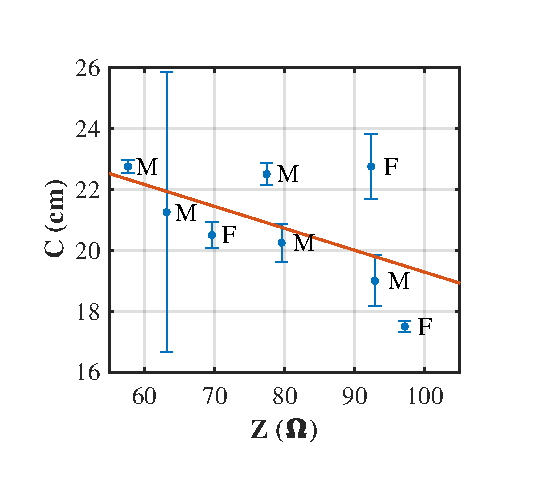
\includegraphics[height=6cm]{figure2a}
		\caption{Relationship between forearm circumference and mean basal impedance}
		\label{fig:C_vs_Z}
	\end{subfigure}%
	~ 
	\begin{subfigure}[t]{0.5\textwidth}
		\centering
		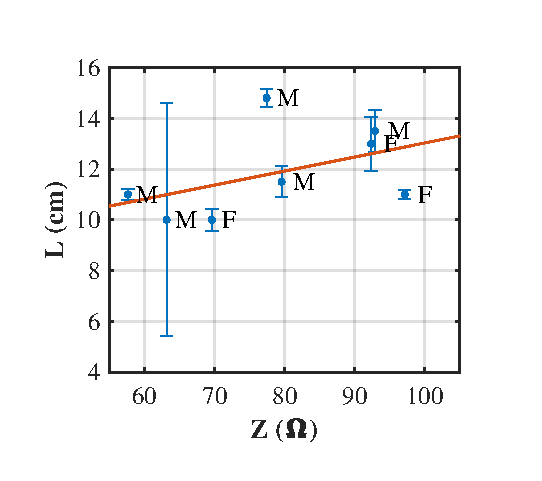
\includegraphics[height=6cm]{figure2b}
		\caption{Relationship between distance sensing electrodes and mean basal impedance}
		\label{fig:l_vs_Z}
	\end{subfigure}
	~ 
	\begin{subfigure}[t]{0.5\textwidth}
		\centering
		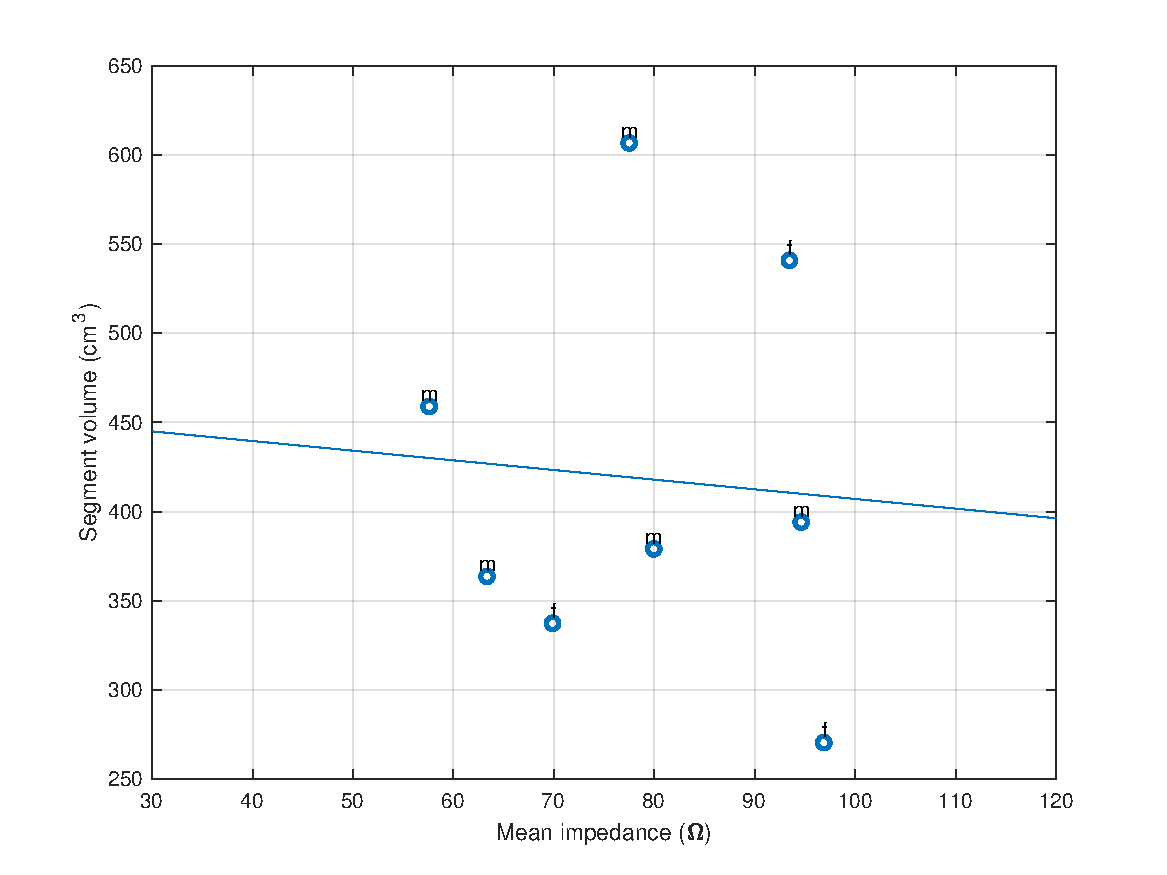
\includegraphics[height=6cm]{figure2c}
		\caption{Relation between forearms segment volume and mean basal resistivity}
		\label{fig:Ve_vs_Z}
	\end{subfigure}
	\caption{Relation between circumference, length and total segment's volume and mean basal impedance}
	\label{fig:relation_geometry_vs_impedance}
\end{figure*}


%%********************************** % Section 5.2.2 ******************************************
\subsection{Mean impedance measurement during venous occlusion}
\label{section results 2.2}
During the following three minutes after the impedance, venous occlusion occurred.\nknote{I think you made an error in explaining what you are trying to say here} As can be seen in figure \ref{fig:rb:all_participants}, all the participants experienced a decrease in basal impedance during this time. Most of the subjects presented a linear impedance decrease trend during the occlusion. However, some of the measurements were clearly affected by motion artefact. Participants one and six are an example of this. 

In participant one, resistance fell immediately as the occlusion occurred. Nevertheless, after a minute the subject moved his arm correcting the trend. Then, impedance continued the trend again. Furthermore,  participant six also showed a similar response when the arm moved. 

Figure \ref{fig:normalise:venous_occlusion} describes how the impedance behaved during the occlusion for all participants. The graph has been normalised to compare the resistivity reduction.  A linear regression was performed in the data to demonstrate the ratio of change during the occlusion.

\begin{figure}[!htbp]
	\centering
	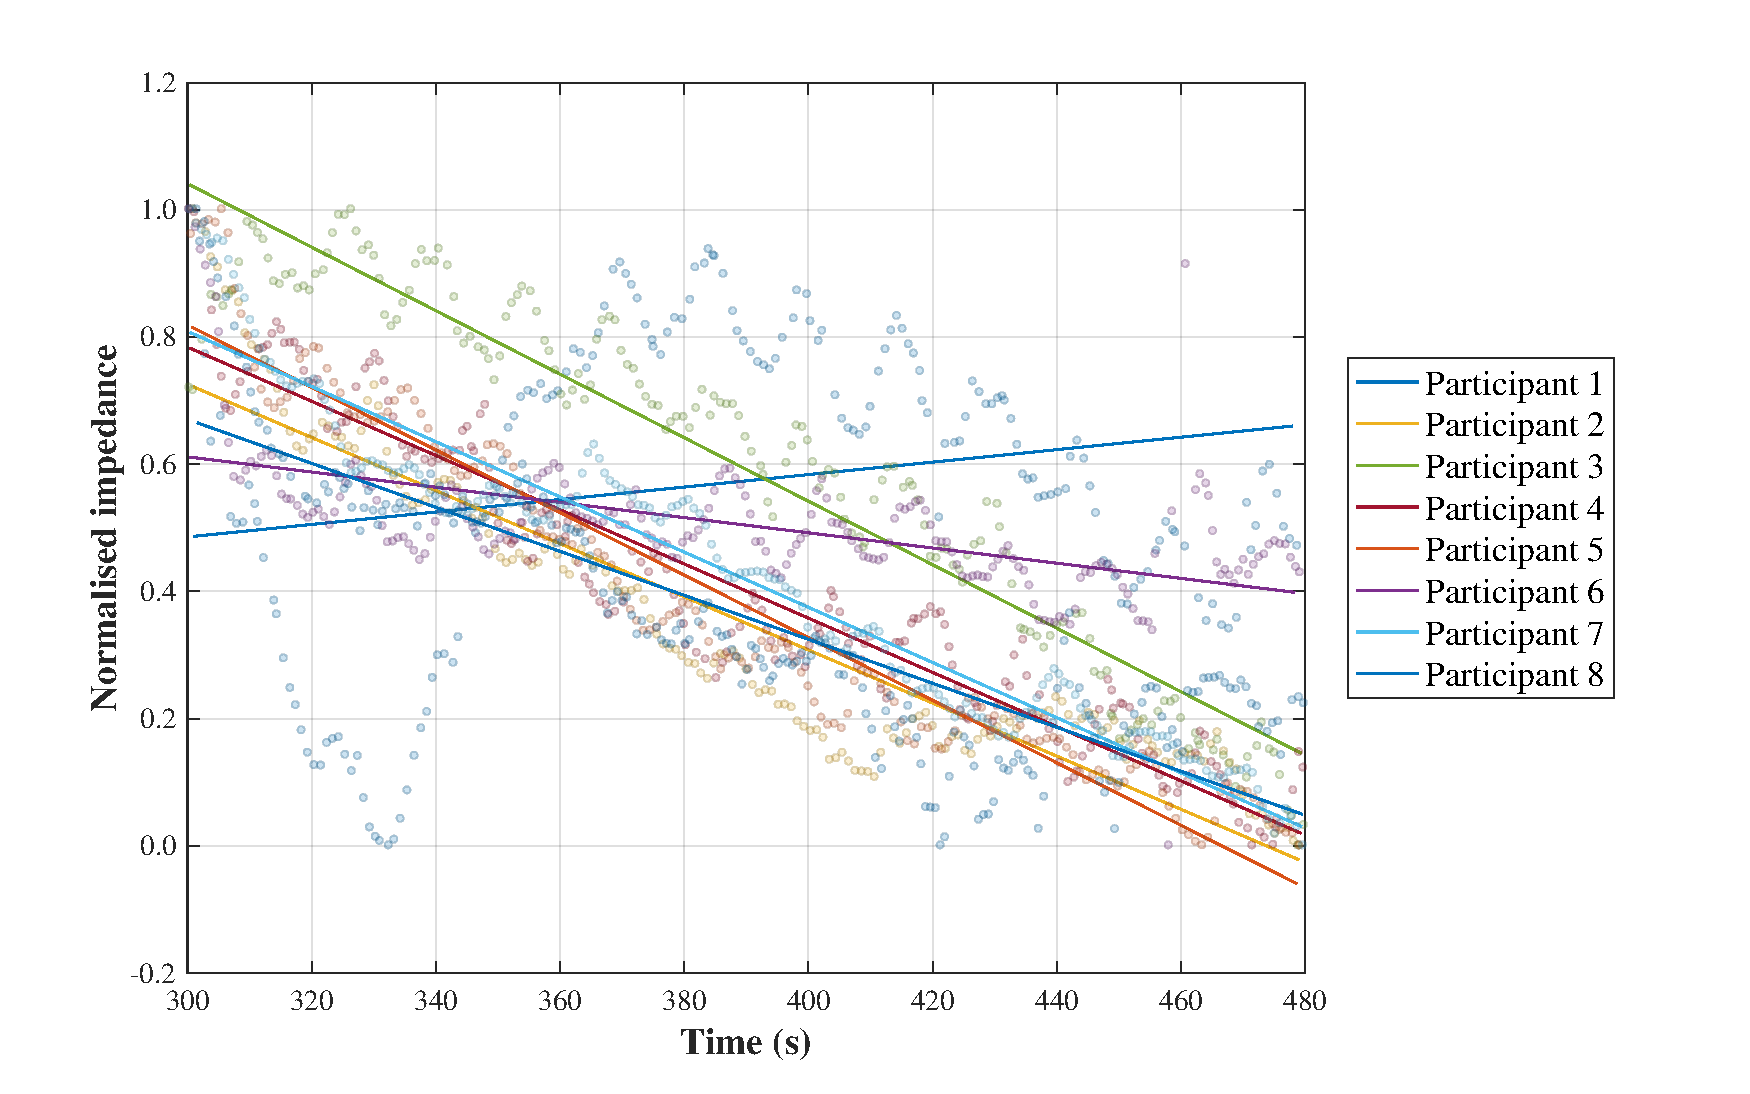
\includegraphics[width=\textwidth,keepaspectratio]{figure3}    
	\caption{Normalise plot of impedance decrease during venous occlusion.}
	\label{fig:normalise:venous_occlusion}
\end{figure}  

The table \ref{tbl:venous_occlusion:region2} overviews the results obtained from the linear regression. The value $Z_1$ illustrates the value of the impedance as the blockage started and $Z_{end}$ the resistance value at the end of the test.  $\Delta Z$ (mean \SI{-0.632(0068)}{\ohm}) is the variation of impedance during the \SI{3}{\minute} that the experiment lasted. The slope demonstrates how much resistance is changing during each beat  (mean $-0.00271\pm3.415e^{-6}\Omega\textrm{/s}$). 

\begin{table}[!htbp]
	\caption{Linear regression result for all participants during venous occlusion.}
	\label{tbl:venous_occlusion:region2}
	\centering
	\begin{tabu}{lcccccc}
		\toprule
		& \textbf{Slope [\si{\ohm/\second}]} & \textbf{Intercept [\si{\ohm}]} & \textbf{$R^2$} & \textbf{$Z_1$ [\si{\ohm}]} & \textbf{$Z_{end}$ [\si{\ohm}]} & \textbf{ $\Delta Z$ [\si{\ohm}]} \\ \midrule
		Participant 1  &   0.00057  &  77.02   &     0.037  &  77.49  &  77.18  &  -0.31\\
		Participant 2  &  -0.00395  &  98.09   &     0.867  &  97.16  &  96.21  &  -0.95\\
		Participant 3  &  -0.00421  &  95.01   &     0.917  &  93.47  &  92.89  &  -0.58\\
		Participant 4  &  -0.00296  &  63.96   &     0.920  &  63.22  &  62.61  &  -0.61\\
		Participant 5  &  -0.00427  &  71.26   &     0.936  &  70.10  &  69.27  &  -0.83\\
		Participant 6  &  -0.00085  &  57.96   &     0.322  &  57.98  &  57.57  &  -0.40\\
		Participant 7  &  -0.00427  &  95.42   &     0.934  &  94.33  &  93.34  &  -0.98\\
		Participant 8  &  -0.00173  &  80.43   &     0.752  &  80.07  &  79.68  &  -0.39\\ \bottomrule
	\end{tabu} 
\end{table}

From the statistical analysis displayed one can conclude the following: as explained previously, the slopes from participants 1 and 6 were affected by the motion artefact. Nevertheless, these trends seemed corrected after one minute of recordings (\SI{360}{\second}). Their slopes were quite far away from the mean value (\num{-0.00271}$\pm$\SI{3.415e-06}{\ohm\per\second}). On the other hand, the rest of the signals showed a similar trend. \mynote{Review this paragraph. It seems to be very similar to the previous one.}


%%********************************** % Section 5.2.3 ******************************************
\subsection{Mean impedance data during partial arterial occlusion}
\label{section results 2.3}
During partial arterial occlusion (\SIrange{480}{760}{\second}), the incoming arterial flow is restricted causing a slow filling of the forearm. This mechanical blocking induces an uncomfortable feeling to the participants, some of them felt numbness in the arm.  As it can be seen from figure \ref{fig:rb:all_participants}, most of the participants there is an apparent drop in impedance during the action. Though participant one moved his muscles creating a sharp fall before releasing the pressure, also partaker four showed a slight increment of impedance followed in the middle of this part of the test. 

Figure \ref{fig:normalise:arterial_occlusion} shows the normalise resistivity decrease for all the participants. Table \ref{tbl:arterial_occlusion:region4} shows the values of the linear regression for the data.   All in all, it is clear that the decrease of resistivity is sharper in this part of the experiment compared to venous occlusion.  In fact, when this data is compared to venous information, the average slope is nearly twice as big (mean \num{-0.00536}$\pm$\SI{2.853e-06}{\ohm\per\second}). Also, the total change of impedance ($\Delta Z$) was almost doubled in all participants, except participant four which value decreased.  

\begin{table}[!htbp]
	\caption{Linear regression result for all participants during partial arterial occlusion.}
	\label{tbl:arterial_occlusion:region4}
	\centering
	\begin{tabu}{lcccccc}
		\toprule
		& \textbf{Slope [\si{\ohm/\second}]} & \textbf{Intercept [\si{\ohm}]} & \textbf{$R^2$} & \textbf{$Z_1$ [\si{\ohm}]} & \textbf{$Z_{end}$ [\si{\ohm}]} & \textbf{ $\Delta Z$ [\si{\ohm}]} \\ \midrule
		Participant 1  &  -0.00656  &   82.44    &   0.519  &  77.51  &  74.91  &  -2.60 \\
		Participant 2  &  -0.00706  &  102.67    &   0.965  &  97.29  &  95.75  &  -1.54 \\
		Participant 3  &  -0.00601  &   98.28    &   0.858  &  93.61  &  92.20  &  -1.41 \\
		Participant 4  &  -0.00327  &   65.05    &   0.474  &  62.25  &  61.81  &  -0.44\\
		Participant 5  &  -0.00767  &   75.89    &   0.989  &  70.05  &  68.50  &  -1.55\\
		Participant 6  &  -0.00366  &   60.53    &   0.939  &  57.74  &  56.88  &  -0.85\\
		Participant 7  &  -0.00490  &   96.64    &   0.969  &  93.11  &  92.02  &  -1.09\\
		Participant 8  &  -0.00381  &   82.54    &   0.627  &  79.70  &  79.10  &  -0.59\\ \bottomrule
	\end{tabu} 
\end{table}

The linear regression of this region of the signal showed an apparent straight tendency for most of the participants. Most of the signals can be represented as negative tilt line ($R^2 \geq 0.858 $), except members one, four and eight ($R^2 \leq 0.627 $).

\mynote{Check about what happens during partial arterial occlusion. Slow filling of the forearm. This information should also be added to the Medical Background}

\begin{figure}[!htbp]
	\centering
	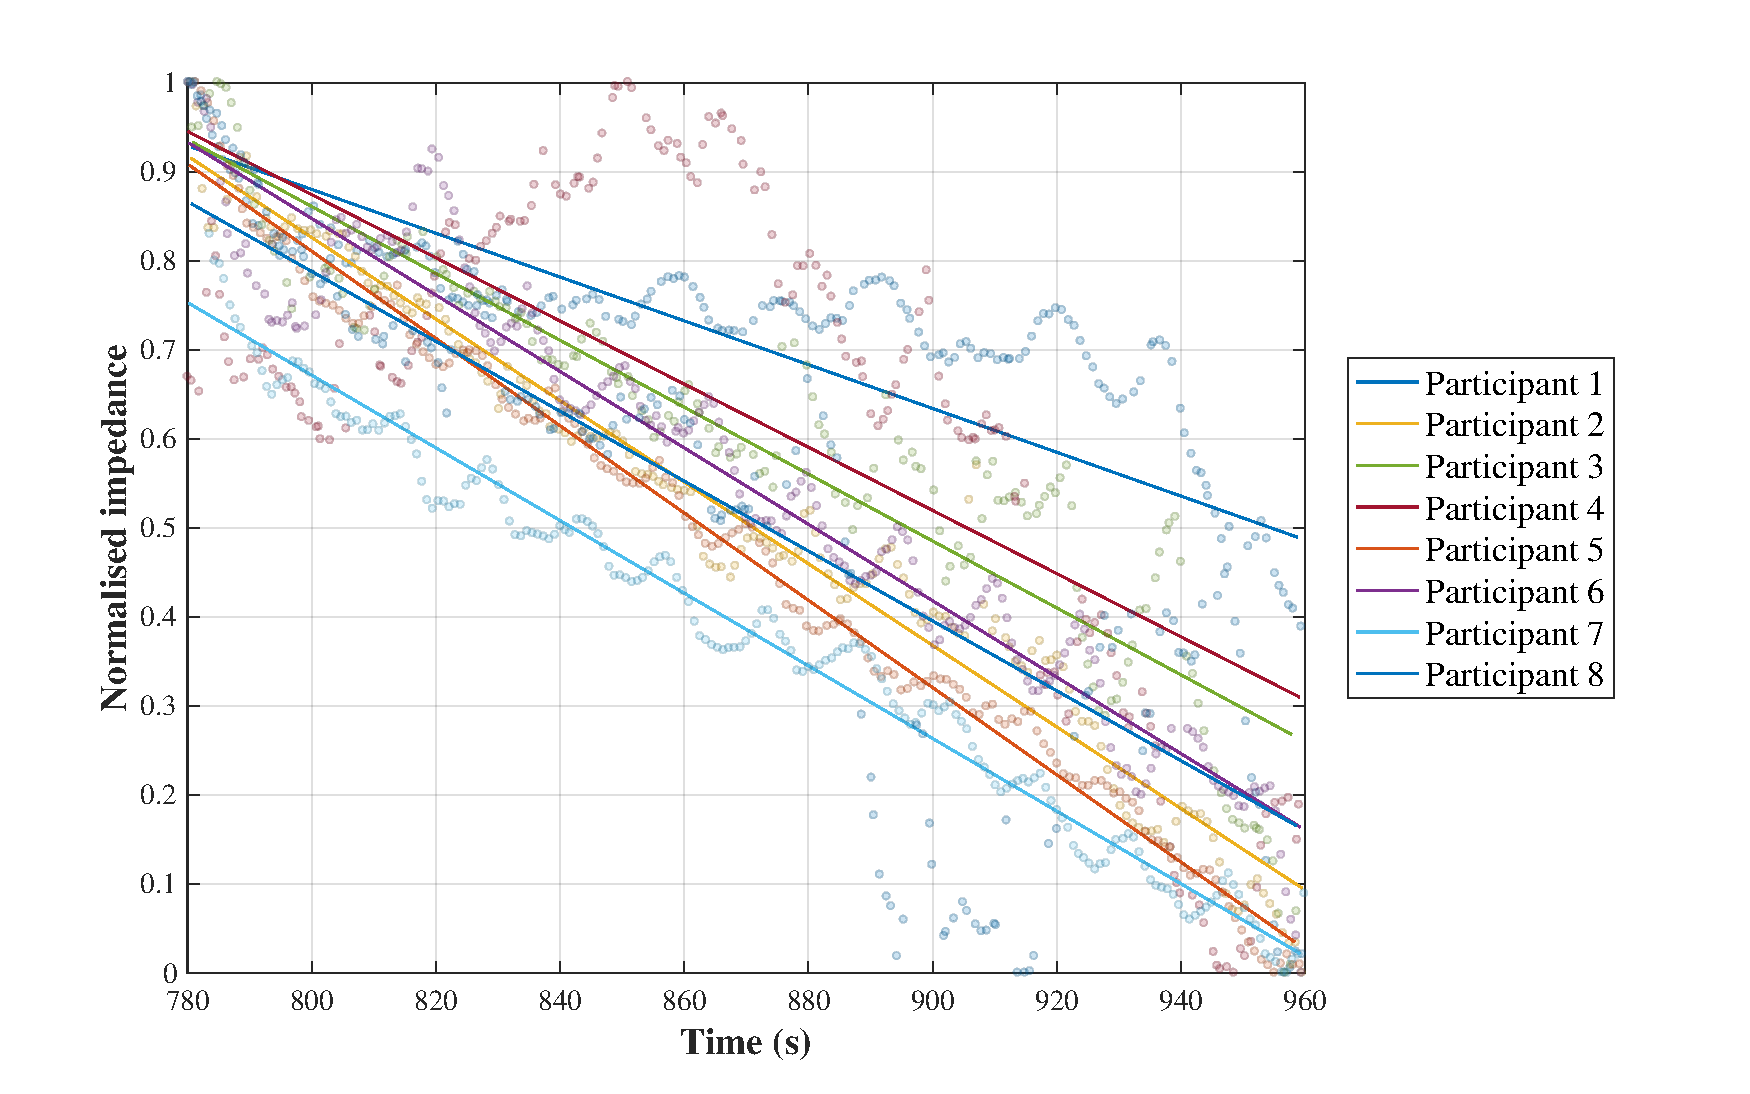
\includegraphics[width=0.9\textwidth,height=0.9\textheight,keepaspectratio]{figure4}    
	\caption{Normalise plot of impedance decrease during partial arterial occlusion.}
	\label{fig:normalise:arterial_occlusion}
\end{figure}
\mynote{Figure \ref{fig:normalise:venous_occlusion} is temporary. It needs to be improved by naming axis}



%%********************************** % Section 5.2.4 ******************************************
\subsection{Mean impedance data during total occlusion}
\label{section results 2.4}
Producing a total occlusion (between \SIrange{1260}{1440}{\second}) in the upper arm stops the blood inflow completely under the obstructed section. This test caused much discomfort on most of the participants, which made them moving their limbs voluntary. Because there is no blood pooling during this part of the experiment is expected not seeing a common tendency in impedance variation. Additionally, the mean restive value is equivalent to the impedance of the tissue components within the segment plus the impedance of the residual blood in the forearm. However, when a change of resistivity happens is mostly caused by the participant's re-accommodation rather than a physiological variable. 

After analysing the data obtained (see  Table \ref{tbl:total_occlusion:region6} and figure \ref{fig:normalise:total_occlusion}), it can be noticed that there is not a defined trend for most of the signals. The slopes and deltas computed show a variation between negative and positive values. Therefore, it can be concluded that there is not an indication of a clear bias common to the signals. 

\begin{table}[!htbp]
	\caption{Linear regression result for all participants during total occlusion.}
	\label{tbl:total_occlusion:region6}
	\centering
	\begin{tabu}{lcccccc}
		\toprule
		& \textbf{Slope [\si{\ohm/\second}]} & \textbf{Intercept [\si{\ohm}]} & \textbf{$R^2$} & \textbf{$Z_1$ [\si{\ohm}]} & \textbf{$Z_{end}$ [\si{\ohm}]} & \textbf{ $\Delta Z$ [\si{\ohm}]} \\ \midrule
		Participant 1  &  -0.00431  &  82.44   &      0.652 &   77.58 &  76.33  &   -1.25\\ 
		Participant 2  &   0.00044  &  96.55   &      0.105 &   97.22 &   97.28 &    0.07\\
		Participant 3  &  -0.00432  &  97.99   &      0.587 &   92.57 &   91.45 &   -1.12\\
		Participant 4  &   0.00226  &  60.31   &      0.789 &   63.31 &   63.45 &    0.14\\
		Participant 5  &  -0.00002  &  69.04   &     -0.005 &   69.22 &   69.01 &   -0.21\\
		Participant 6  &  -0.00096  &  58.38   &      0.457 &   57.34 &   56.95 &   -0.40\\
		Participant 7  &   0.00310  &  88.70   &      0.899 &   92.78 &   93.11 &    0.33\\
		Participant 8  &  -0.00080  &  79.94   &      0.644 &   78.97 &   78.82 &   -0.15\\ \bottomrule
	\end{tabu} 
\end{table}

The impedance plethysmography signal can confirm the absence of blood flow. On section xxx \mynote{Add reference in plethysmography that shows the waveforms} is shown the lack of peaks in the signal. 

\mynote{Check about what happens during partial arterial occlusion. Slow filling of the forearm. This information should also be added to the Medical Background}

\begin{figure}[!htbp]
	\centering
	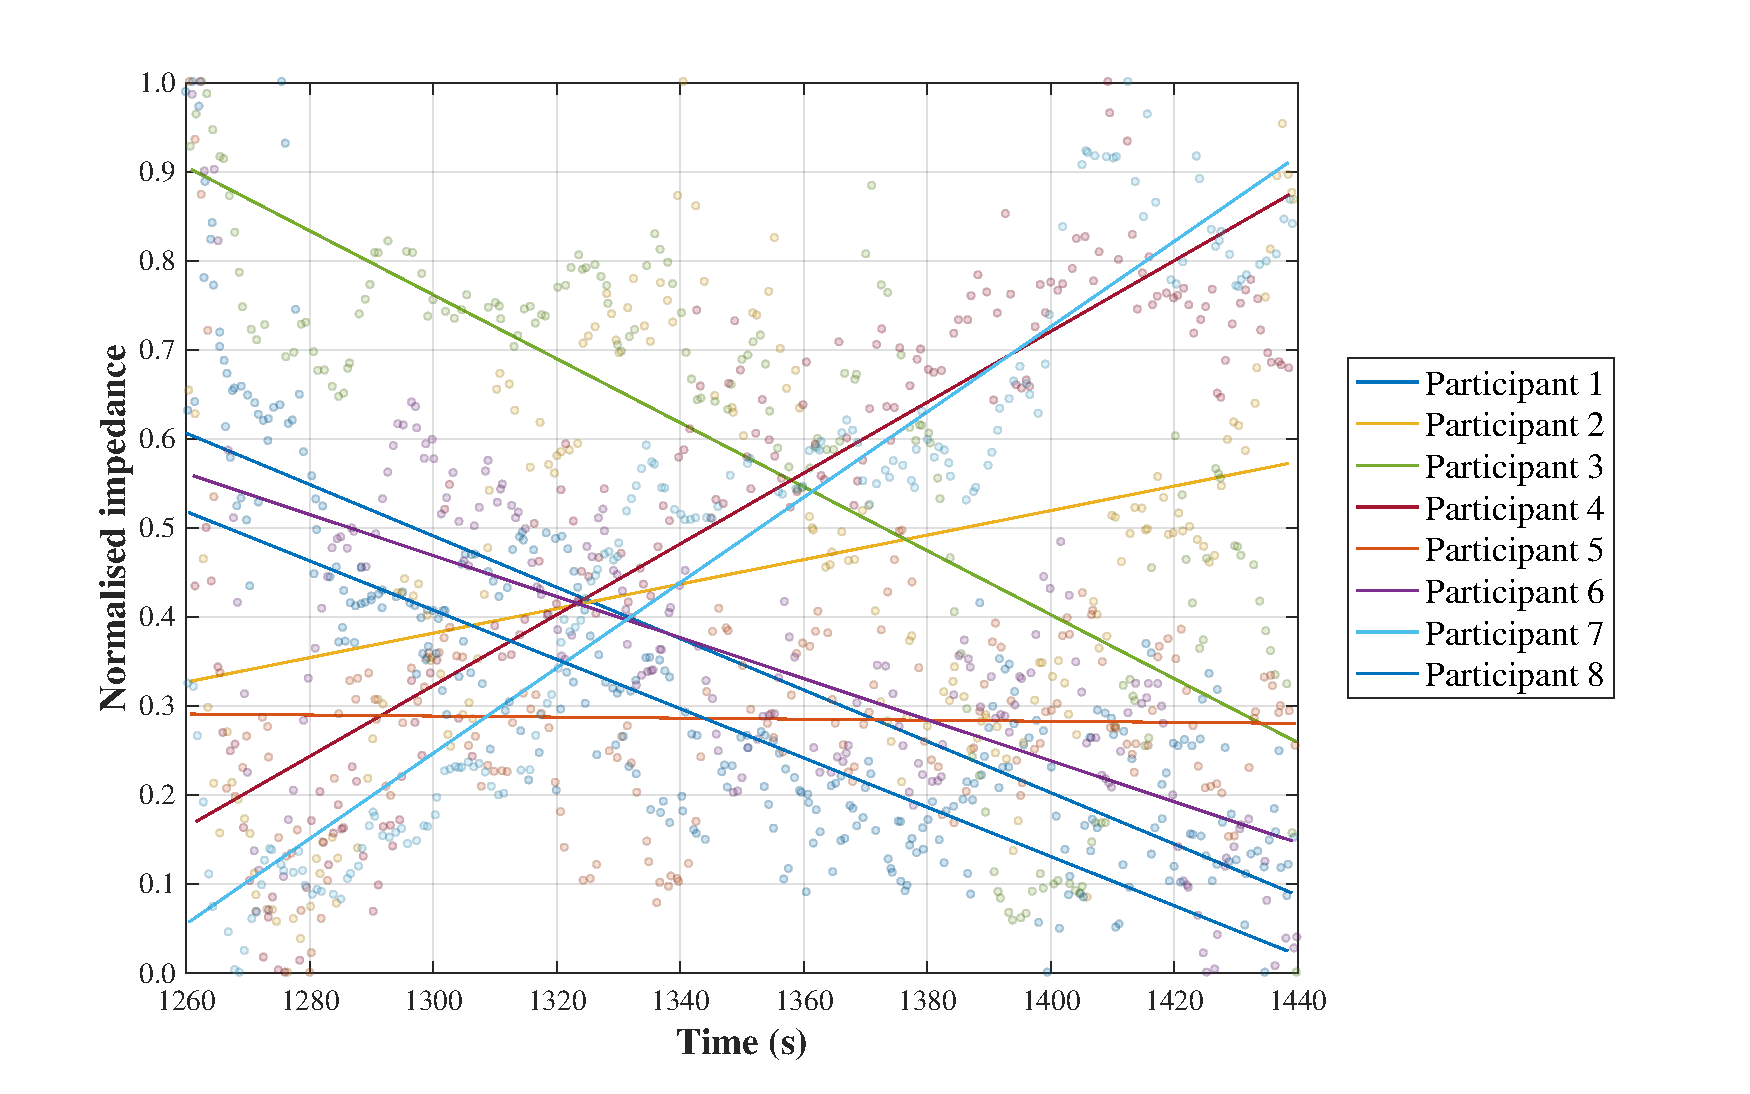
\includegraphics[width=0.9\textwidth,height=0.9\textheight,keepaspectratio]{figure5}    
	\caption{Normalise plot of impedance decrease during total occlusion.}
	\label{fig:normalise:total_occlusion}
\end{figure}
\mynote{Figure \ref{fig:normalise:venous_occlusion} is temporary. It needs to be improved by naming axis}


%%********************************** % Section 5.3 ******************************************
%\pagebreak
\section{Plethysmography impedance results}
\label{section results 3}
The iPG device provided a port illustrated as $Z_{AC}$ \mynote{To double check if this is the correct port name from the initial description} which provided a high-resolution view of the plethysmography waveform.  In fact, as shown in the design section xxx \mynote{Reference a section to this part}, the signal was amplified nearly 2500 times. Hence, the waveform obtained provides more detail and also improves rejection to noise.

The waveforms obtained through this method reproduce the change of volume per heart beat within the sensing electrodes. The filling of the blood vessels creates small changes in resistivity that change with the circulatory cycle (see section xxx \mynote{I have to add a section to describe how plethysmography is related to blood cycle}). The waveforms presented in this part were analysed using the decomposing method describe in section \ref{section procedure 3.2}. \mynote{I need to add more detail within that section}. Five different points on the waveform were identified by the algorithm.

The waveform produced by the device is inverted as represented by various other plethysmography devices such as photoplethysmography. During the systolic cycle, the blood vessels expand allowing more blood volume. Hence, the impedance drops proportionally to the amount of blood because the forearm's segment is more electrically conductive. On the other hand, during the diastolic cycle, blood vessels empty causing a reduction the quantity of blood contained in the segment. As a result, the impedance increases.  

Treating the digital signal required to remove noisy components of the waveform. As described in section xxx\mynote{Add section were the digital processing was performed}, the signal was levelled to zero.  From there, the points of interest were calculated to identify the different changes in the waveform. The analysis of the plethysmographic wave was performed by averaging all the waveform detected by the algorithm. The following discussion represents the change of form from non-occlusion state to an occluded one. At the end of the section, the result of all participants will be summarised \mynote{I could add a description of how the signal looks. For instance by adding 10 or 20 beats to show how the device worked.}.

%%********************************** % Section 5.3.1 ******************************************
\subsection{Plethysmography waveform change from baseline to venous occlusion}
\label{section results 3.1}
This analysis corresponds to the waveform during baseline (\SIrange{0}{300}{\second}), venous occlusion (\SIrange{300}{480}{\second}) and return to control signal (\SIrange{480}{780}{\second}). This graph was obtained by averaging all the plethysmography waveforms detected by the algorithm and described in detail in section xxx \mynote{Add reference where the waveform detection algorithm is explained}. In the end, all the peaks were averaged obtaining the mean waveform displayed in the figure for baseline and venous occlusion.

Figure \ref{fig:iPG_venous_baseline} shows the common impedance plethysmography waveform, with indicators of their amplitudes at different points of interest. The distance between systolic peak (Point A) to dicrotic notch (Point B) and diastolic peak (Point C) was calculated. This value was later transposed into the occlusion wave to identify their values during the venous occlusion test.

As detailed in section xxx \mynote{Add note describing how the waveform is composed}, a plethysmography waveform consists of three distinct parts. The systolic peak, dicrotic notch and the diastolic peak, which have been indicated in the figure \ref{fig:iPG_venous_baseline}. From a qualitative point of view, it can be noticed that there is a difference in the morphology of the waveform. An analysis on the change of each these points are presented in figure \ref{fig:iPG_change_points_venous} and analysed in detail as follows.

\begin{figure*}[!htbp]
	\centering
	\begin{subfigure}[t]{0.5\textwidth}
		\centering
		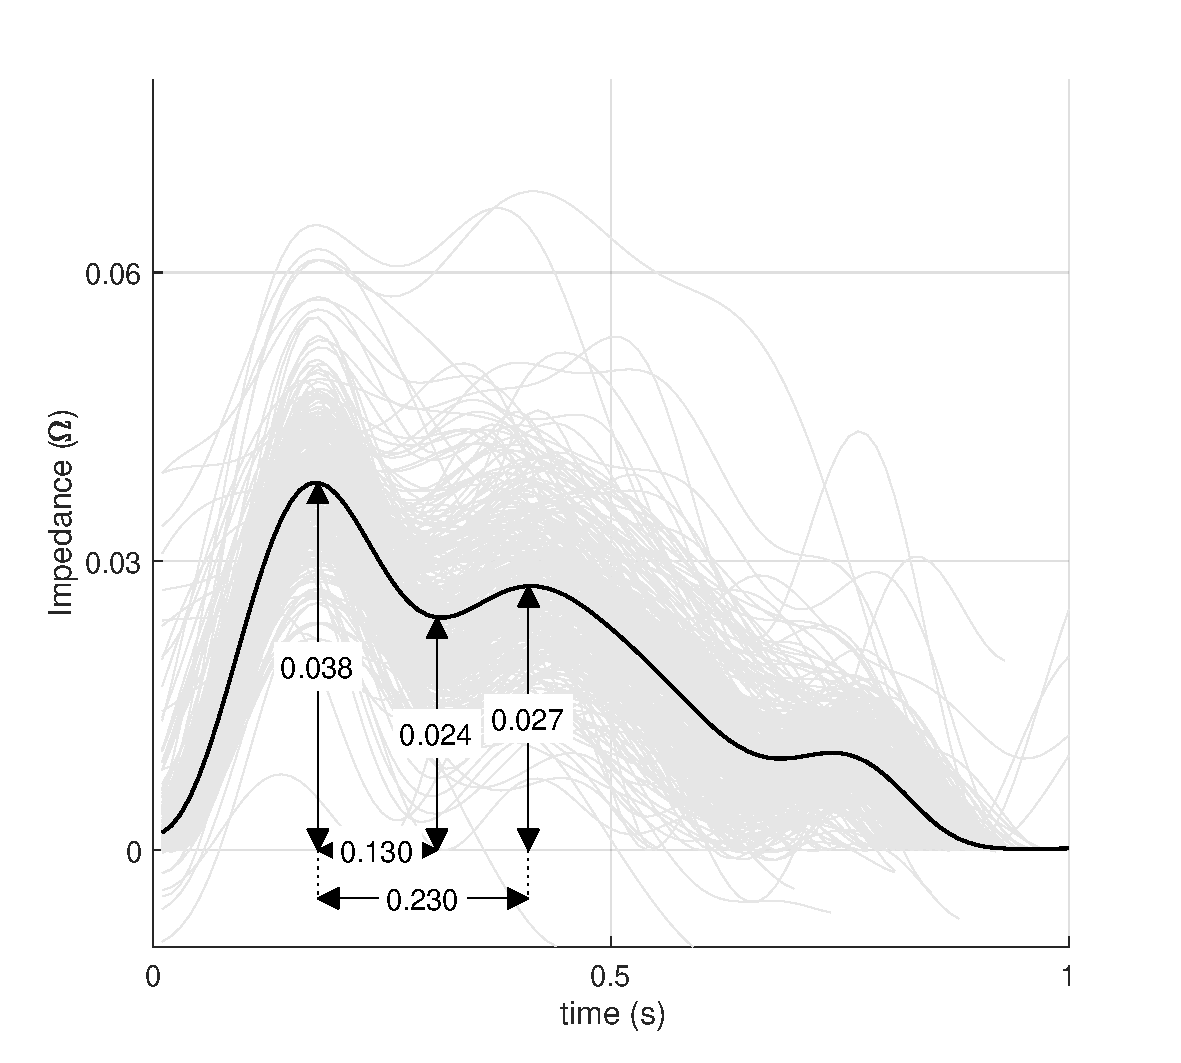
\includegraphics[height=7.6cm]{figure6a}
		\caption{Average plethysmography waveform for baseline region 1 (\SIrange{0}{300}{\second})}
		\label{fig:iPG_venous_baseline}
	\end{subfigure}%
	~ 
	\begin{subfigure}[t]{0.5\textwidth}
		\centering
		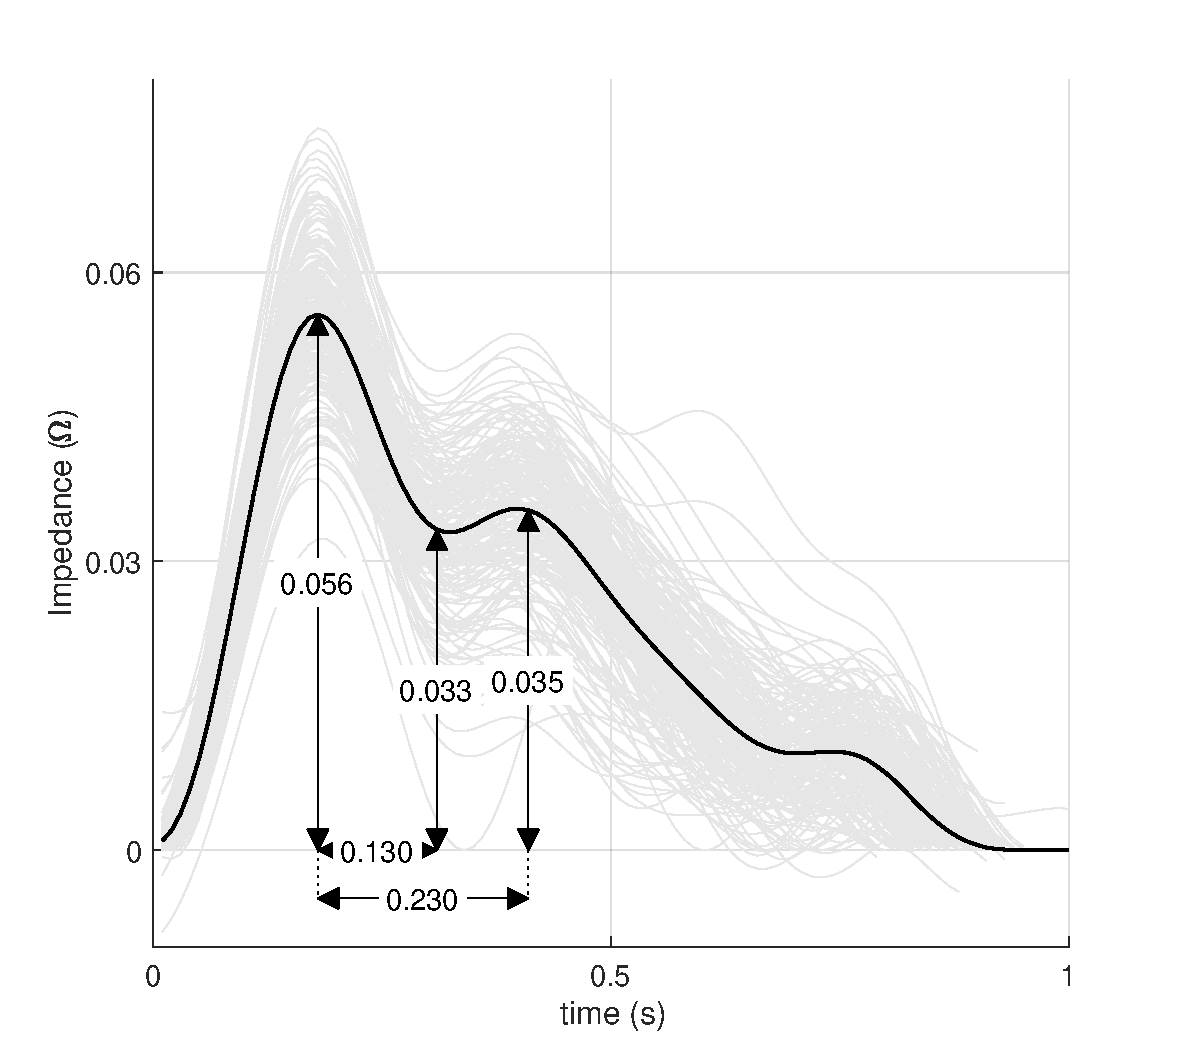
\includegraphics[height=7.6cm]{figure6b}
		\caption{Average plethysmography waveform during venous occlusion region 2 (\SIrange{300}{480}{\second})}
		\label{fig:iPG_venous_occlusion}
	\end{subfigure}
	\caption{Plethysmography waveform of the participant seven between baseline and venous occlusion}
	\label{fig:iPG_venous}
\end{figure*}

\begin{figure*}[h]
	\centering
	\begin{subfigure}[t]{0.5\textwidth}
	\centering
		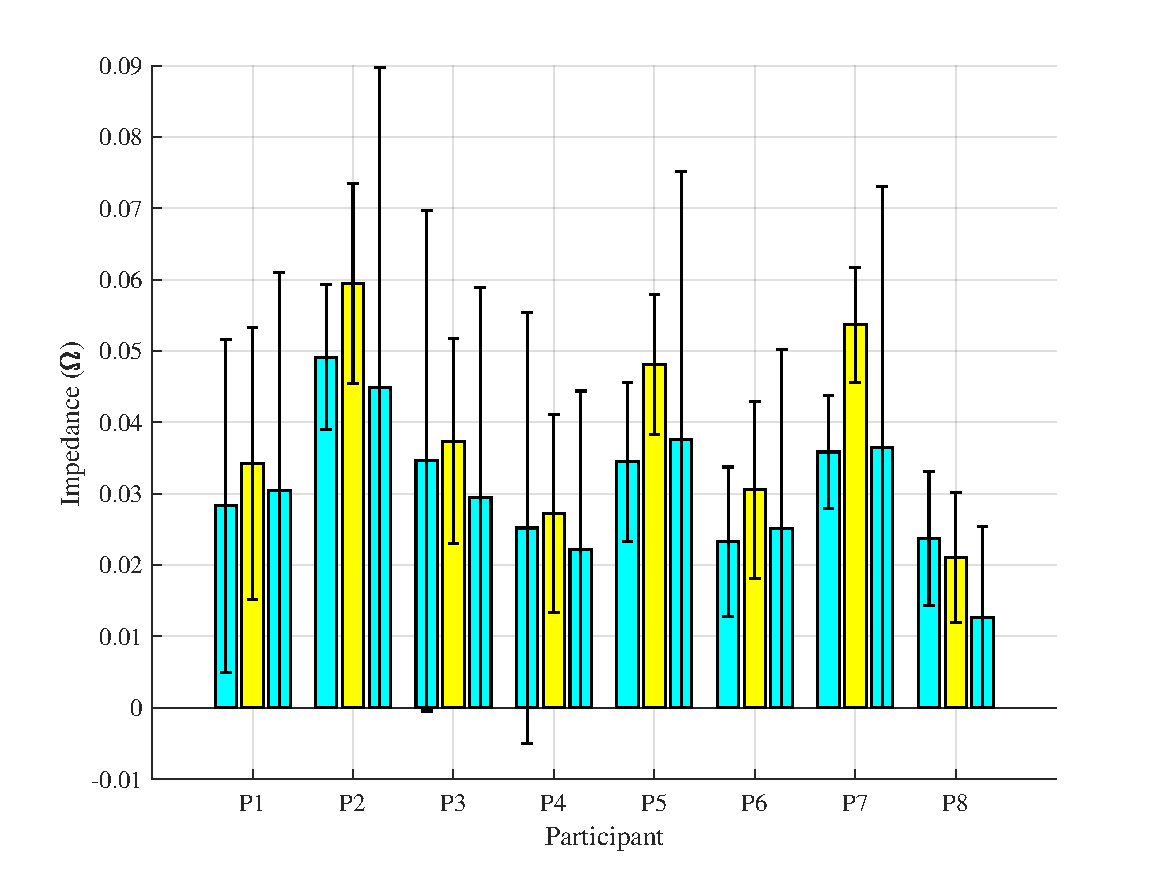
\includegraphics[height=6cm,keepaspectratio]{figure7a}    
		\caption{Change of amplitude of the waveform at point A.}
		\label{fig:change_A_venous}
	\end{subfigure}%
	~ 
	\begin{subfigure}[t]{0.5\textwidth}
		\centering
		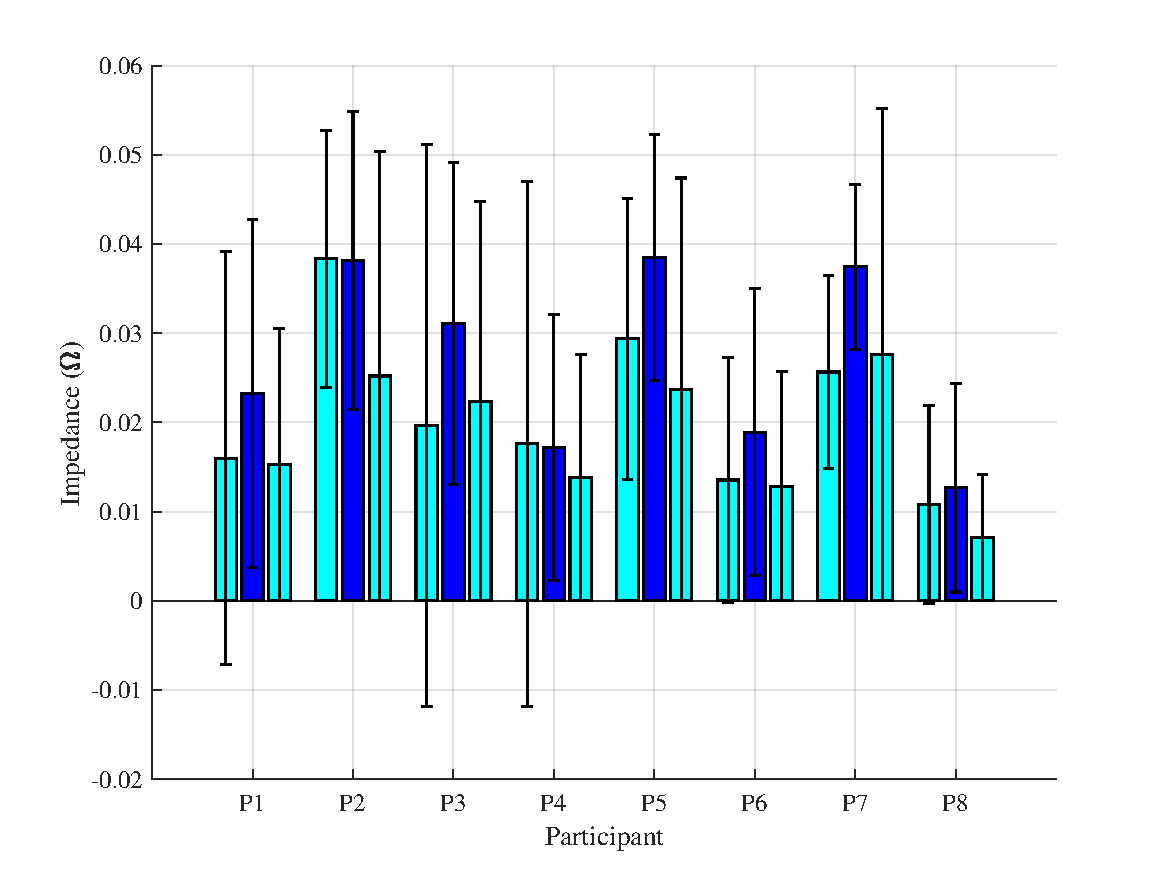
\includegraphics[height=6cm,keepaspectratio,keepaspectratio]{figure7b}    
		\caption{Change of amplitude of the waveform at point B}
		\label{fig:change_B_venous}
	\end{subfigure}
	~
	\begin{subfigure}[t]{0.5\textwidth}
		\centering
		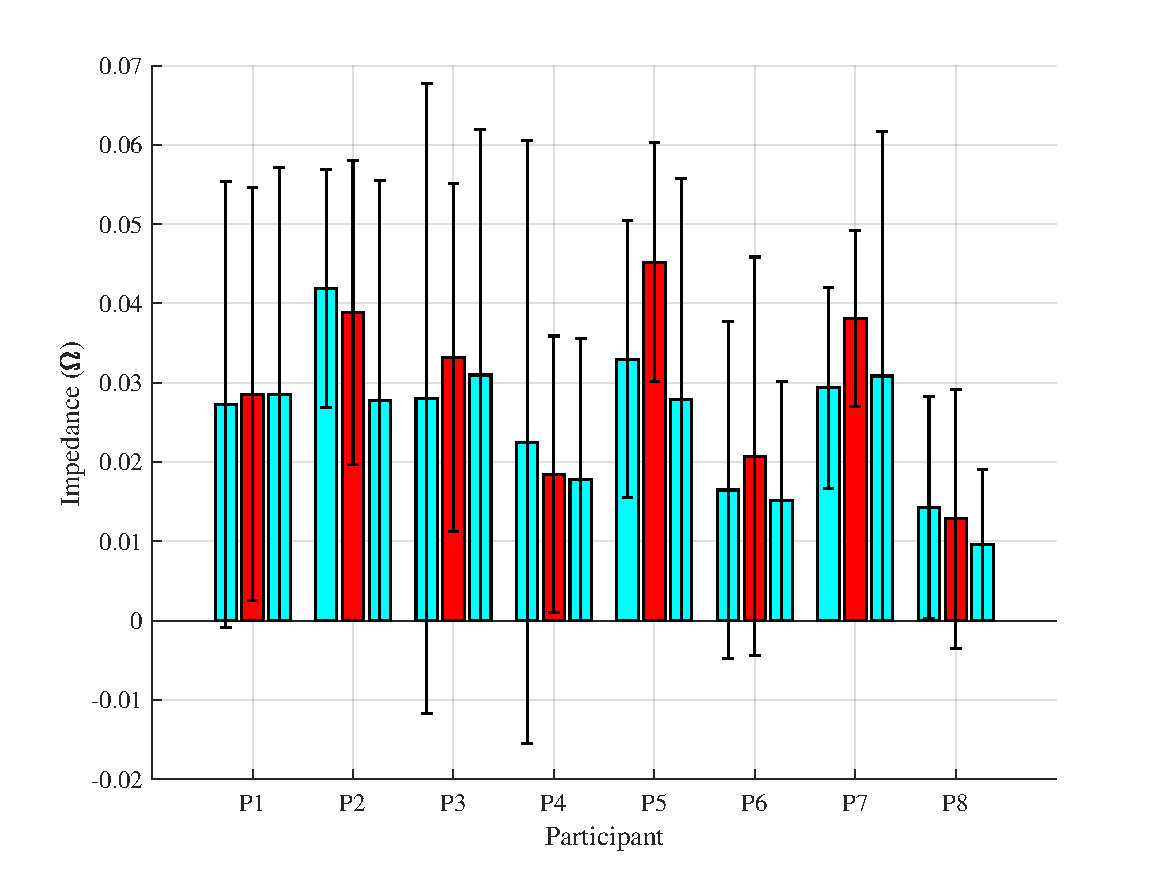
\includegraphics[height=6cm,keepaspectratio]{figure7c}    
		\caption{Change of amplitude of the waveform at point C}
		\label{fig:change_C_venous}
\end{subfigure}%
	\caption{Changes of the impedance peak values during baseline, partial arterial occlusion and return to baseline for points A,B and C.}
	\label{fig:iPG_change_points_venous}
\end{figure*}

\subsubsection{Changes in systolic peak (Point A)}
\label{section results 3.1.1}
Most of the signals showed a change on the height of their top systolic values after inflating the cuff to the values shown in column \textit{Occlusion 1} in Table~\ref{tbl:occlusions}. After quantifying the amplitude of the signal at this point, it can be seen an increase in their peak value. Indeed \SI{87}{\percent} of the participants showed an increment in resistance with an average of \SI{20.93}{\percent}, only participant 8 was an exception which impedance decreased \SI{-11.11}{\percent}. Then, when cuff's pressure was released, all the participants showed a decline of the peak value with an average of \SI{-27.88}{\percent}, returning to similar values previous the occlusion. Figure \ref{fig:change_A_venous} indicates the relation of change in amplitude during the three conditions. 

\begin{table}[!htbp]
	\caption{Change of amplitude of the waveform at peak A during the transition from baseline to venous occlusion.}
	\label{tbl:change_A_venous}
	\centering\small
\begin{tabular}{l
				*{3}{S[table-format=1.4]@{\,\( \pm \)\,}S[table-format=1.4]} %Format for Z+-std
		       cc}
	\toprule
	& \multicolumn{2}{c}{\multirow{2}{*}{\textbf{Baseline [\si{\ohm}]}}}
	& \multicolumn{2}{c}{\multirow{2}{*}{\textbf{Occlusion [\si{\ohm}]}}}
	& \multicolumn{2}{c}{\multirow{2}{*}{\textbf{Baseline [\si{\ohm}]}}}
	& \multicolumn{2}{c}{\textbf{Change}} \\
	& \multicolumn{2}{c}{}
	& \multicolumn{2}{c}{}
	& \multicolumn{2}{c}{}
	&\textbf{R1-R2}&\textbf{R2-R3}\\\midrule
	Participant 1    &     0.0283    &     0.0233    &     0.0342    &     0.0191    &     0.0305    &     0.0305    &      20.93\%    &     -13.29\%    \\
	Participant 2    &     0.0491    &     0.0102    &     0.0595    &     0.0140    &     0.0449    &     0.0449    &      21.01\%    &     -29.68\%    \\
	Participant 3    &     0.0346    &     0.0351    &     0.0374    &     0.0144    &     0.0294    &     0.0294    &       7.91\%    &     -22.89\%    \\
	Participant 4    &     0.0252    &     0.0303    &     0.0272    &     0.0139    &     0.0222    &     0.0222    &       7.98\%    &     -19.87\%    \\
	Participant 5    &     0.0345    &     0.0112    &     0.0481    &     0.0098    &     0.0376    &     0.0376    &      39.68\%    &     -30.69\%    \\
	Participant 6    &     0.0233    &     0.0105    &     0.0306    &     0.0124    &     0.0251    &     0.0251    &      31.33\%    &     -23.52\%    \\
	Participant 7    &     0.0359    &     0.0080    &     0.0537    &     0.0081    &     0.0365    &     0.0365    &      49.72\%    &     -47.78\%    \\
	Participant 8    &     0.0237    &     0.0094    &     0.0211    &     0.0091    &     0.0127    &     0.0127    &     -11.11\%    &     -35.30\%    \\  \bottomrule
\end{tabular} 
\end{table}


\subsubsection{Changes in dicrotic notch peak (Point B)}
\label{section results 3.1.2}
The dicrotic notch point is located between the systolic and diastolic peaks. In the forearm's iPG waveform looks like a dip as illustrated figure \ref{fig:iPG_venous}. This locality in the waveform has been identified in this document as point B. 

The value of this signal changed from baseline when the venous occlusion happened. After that, when cuff was deflated, all impedance peaks decreased. According to the data shown on Table \ref{tbl:change_B_venous}, it can be noticed that most of the signals (\SI{75}{\percent}) shown an increase in their value. Certainly, there was an increment in impedance on average of \SI{29.30}{\percent}. However, partakers two and four noted a slight decrease in their values \SI{-0.47}{\percent} and \SI{-2.34}{\percent} which were not very significant compared to the others. In contrast, after releasing the pressure, all signals experience a reduction of their peak value (mean \SI{41.47}{\percent}).

\begin{table}[!htbp]
	\caption{Change of amplitude of the waveform at peak B during the transition from baseline to venous occlusion.}
	\label{tbl:change_B_venous}
	\centering\small
	\begin{tabular}{l
					*{3}{S[table-format=1.4]@{\,\( \pm \)\,}S[table-format=1.4]} %Format for Z+-std
					cc}
	\toprule
	& \multicolumn{2}{c}{\multirow{2}{*}{\textbf{Baseline [\si{\ohm}]}}}
	& \multicolumn{2}{c}{\multirow{2}{*}{\textbf{Occlusion [\si{\ohm}]}}}
	& \multicolumn{2}{c}{\multirow{2}{*}{\textbf{Baseline [\si{\ohm}]}}}
	& \multicolumn{2}{c}{\textbf{Change}} \\
	& \multicolumn{2}{c}{}
	& \multicolumn{2}{c}{}
	& \multicolumn{2}{c}{}
	&\textbf{R1-R2}&\textbf{R2-R3}\\\midrule
	Participant 1    &     0.0160    &     0.0231    &     0.0232    &     0.0195    &     0.0153    &     0.0153    &     45.07    \%      &     -49.54    \%      \\  
	Participant 2    &     0.0383    &     0.0144    &     0.0382    &     0.0167    &     0.0252    &     0.0252    &     -0.47    \%      &     -33.78    \%      \\  
	Participant 3    &     0.0196    &     0.0315    &     0.0311    &     0.0181    &     0.0224    &     0.0224    &     58.38    \%      &     -44.40    \%      \\  
	Participant 4    &     0.0176    &     0.0294    &     0.0172    &     0.0149    &     0.0138    &     0.0138    &     -2.34    \%      &     -19.25    \%      \\  
	Participant 5    &     0.0294    &     0.0158    &     0.0385    &     0.0138    &     0.0237    &     0.0237    &     31.07    \%      &     -50.37    \%      \\  
	Participant 6    &     0.0135    &     0.0138    &     0.0189    &     0.0161    &     0.0128    &     0.0128    &     39.49    \%      &     -44.62    \%      \\  
	Participant 7    &     0.0256    &     0.0108    &     0.0374    &     0.0092    &     0.0276    &     0.0276    &     45.94    \%      &     -38.44    \%      \\  
	Participant 8    &     0.0108    &     0.0111    &     0.0127    &     0.0117    &     0.0071    &     0.0071    &     17.28    \%      &     -51.42    \%      \\ \bottomrule
	\end{tabular} 
\end{table}

\subsubsection{Changes in diastolic peak (Point C)}
\label{section results 3.1.3}
The diastolic peak corresponds to the point C of the waveform. Figure \ref{fig:change_C_venous} shows that there is not a clear trend compared to the other spots previously examined. In fact, three participants experience a decline in the impedance at this point with an average drop of \SI{-11.74}{\percent} and the rest experienced an increase of impedance had a rise an average of \SI{23}{\percent}. Table \ref{tbl:change_C_venous} shows the mean values of the impedance at this place. At this point, it is not possible to get a conclusion about the trend of this point of data. In contrast, after releasing the upper arm's pressure, most participants experience a decrease in their diastolic peak impedance, with an average of \SI{-24}{\percent}. Participant one was the only one that did not register any significant change. 

\begin{table}[!htbp]
	\caption{Change of amplitude of the waveform at peak C during the transition from baseline to venous occlusion.}
	\label{tbl:change_C_venous}
	\centering\small
	\begin{tabular}{l
					*{3}{S[table-format=1.4]@{\,\( \pm \)\,}S[table-format=1.4]} %Format for Z+-std
					cc}
	\toprule
	& \multicolumn{2}{c}{\multirow{2}{*}{\textbf{Baseline [\si{\ohm}]}}}
	& \multicolumn{2}{c}{\multirow{2}{*}{\textbf{Occlusion [\si{\ohm}]}}}
	& \multicolumn{2}{c}{\multirow{2}{*}{\textbf{Baseline [\si{\ohm}]}}}
	& \multicolumn{2}{c}{\textbf{Change}} \\
	& \multicolumn{2}{c}{}
	& \multicolumn{2}{c}{}
	& \multicolumn{2}{c}{}
	&\textbf{R1-R2}&\textbf{R2-R3}\\\midrule
	Participant 1    &     0.0272    &     0.0281    &     0.0285    &     0.0260    &     0.0286    &     0.0286    &       4.79    \%      &       0.03    \%      \\  
	Participant 2    &     0.0419    &     0.0150    &     0.0389    &     0.0191    &     0.0278    &     0.0278    &      -7.17    \%      &     -26.57    \%      \\  
	Participant 3    &     0.0280    &     0.0397    &     0.0332    &     0.0219    &     0.0310    &     0.0310    &      18.37    \%      &      -7.80    \%      \\  
	Participant 4    &     0.0225    &     0.0380    &     0.0185    &     0.0174    &     0.0178    &     0.0178    &     -17.99    \%      &      -2.94    \%      \\  
	Participant 5    &     0.0330    &     0.0175    &     0.0452    &     0.0151    &     0.0279    &     0.0279    &      37.18    \%      &     -52.58    \%      \\  
	Participant 6    &     0.0165    &     0.0212    &     0.0207    &     0.0251    &     0.0151    &     0.0151    &      25.96    \%      &     -34.25    \%      \\  
	Participant 7    &     0.0294    &     0.0127    &     0.0381    &     0.0111    &     0.0309    &     0.0309    &      29.85    \%      &     -24.77    \%      \\  
	Participant 8    &     0.0143    &     0.0140    &     0.0129    &     0.0163    &     0.0096    &     0.0096    &     -10.06    \%      &     -23.09    \%      \\  
	\bottomrule
	\end{tabular} 
\end{table}

%%********************************** % Section 5.3.2 ******************************************
\subsection{Plethysmography waveform change during partial arterial occlusion}
\label{section results 3.2}
During this type of occlusion, most of the signals also showed a modification on the height of their top systolic values. The analysis of this section resembles the baseline time in region 3 (\SIrange{480}{780}{\second}), three minutes of partial venous occlusion in region 4 (\SIrange{780}{960}{\second}) and return to baseline region 5 (\SIrange{960}{1260}{\second}). The cuff was inflated to the pressure presented in the column \textit{Occlusion 2} in Table \ref{tbl:occlusions}. 

Figure \ref{fig:iPG_change_points_arterial} shows the average waveform in baseline and during occlusion for participant seven. As it can be seen from the graph, it is apparent that there is an increase in the systolic peak (point A) and a reduction in the diastolic peak point C). Figure \ref{fig:iPG_change_points_arterial} also features the impedance change in each participant. The following sections will describe in detail the changes to each of the spots. 

\begin{figure*}[!htbp]
	\centering
	\begin{subfigure}[t]{0.5\textwidth}
		\centering
		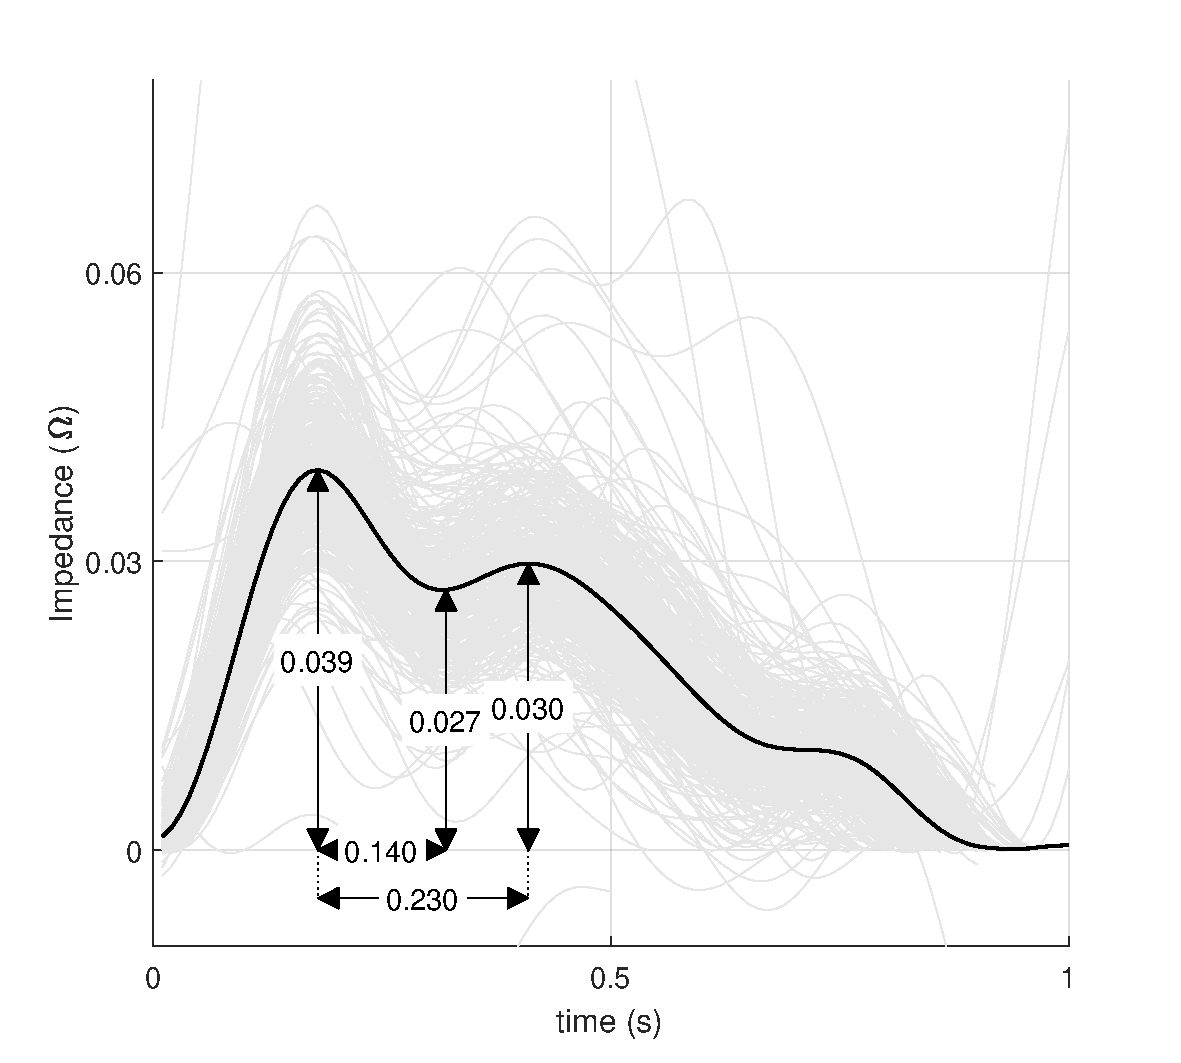
\includegraphics[height=7.6cm]{figure8a}
		\caption{Average plethysmography waveform during venous occlusion region 3 (\SIrange{480}{780}{\second})}
		\label{fig:iPG_arterial_baseline}
	\end{subfigure}%
	~ 
	\begin{subfigure}[t]{0.5\textwidth}
		\centering
		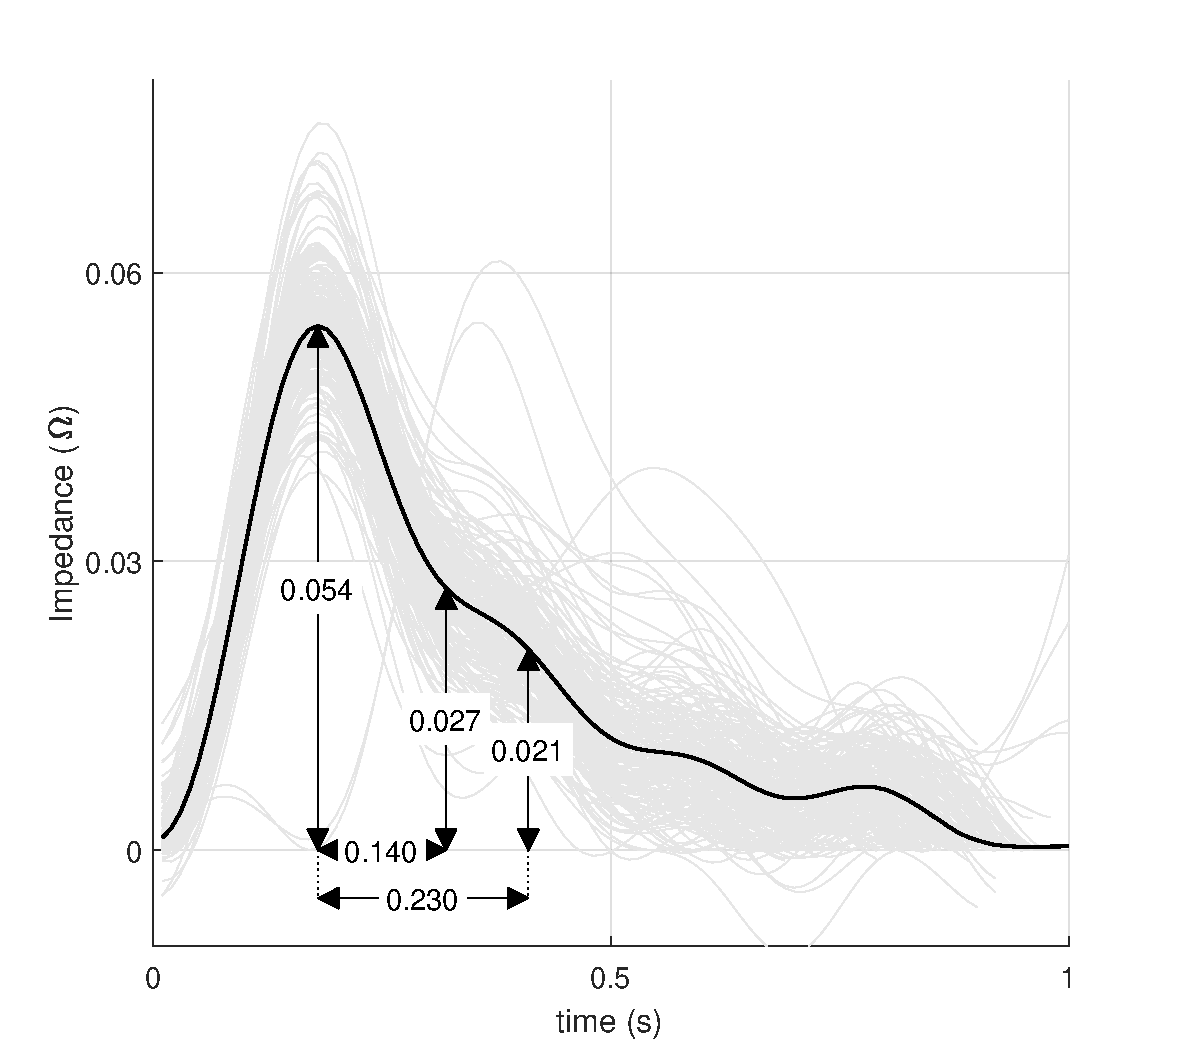
\includegraphics[height=7.6cm]{figure8b}
		\caption{Average plethysmography waveform during venous occlusion region 4 (\SIrange{780}{960}{\second})}
		\label{fig:iPG_arterial_occlusion}
	\end{subfigure}
	\caption{Plethysmography waveform of the participant seven between baseline and partial arterial occlusion}
	\label{fig:iPG_arterial}
\end{figure*}

\begin{figure*}[!htbp]
	\centering
	\begin{subfigure}[t]{0.5\textwidth}
		\centering
		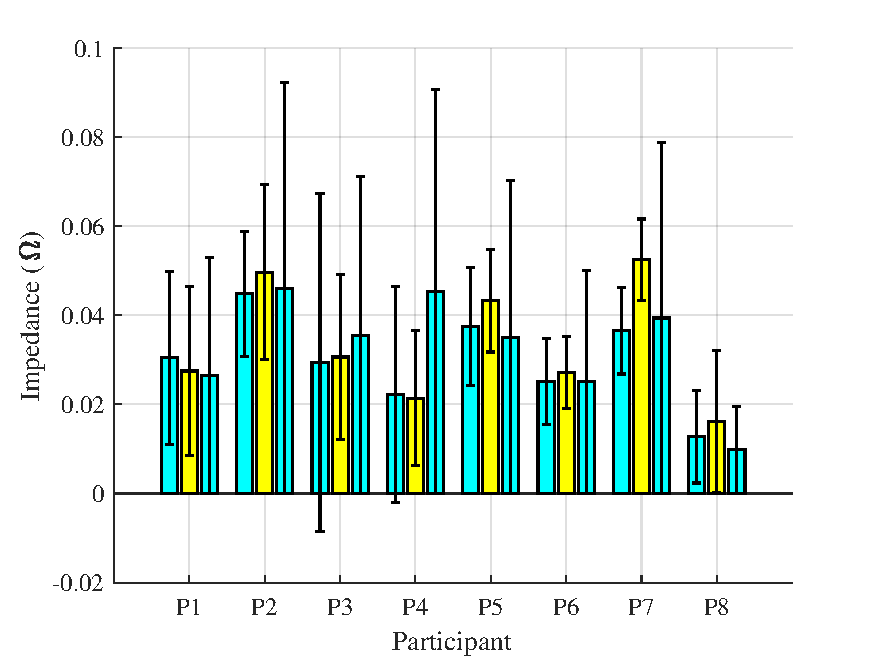
\includegraphics[height=6cm,keepaspectratio]{figure9a}    
		\caption{Change of amplitude of the waveform at point A.}
		\label{fig:change_A_arterial}
	\end{subfigure}%
	~ 
	\begin{subfigure}[t]{0.5\textwidth}
		\centering
		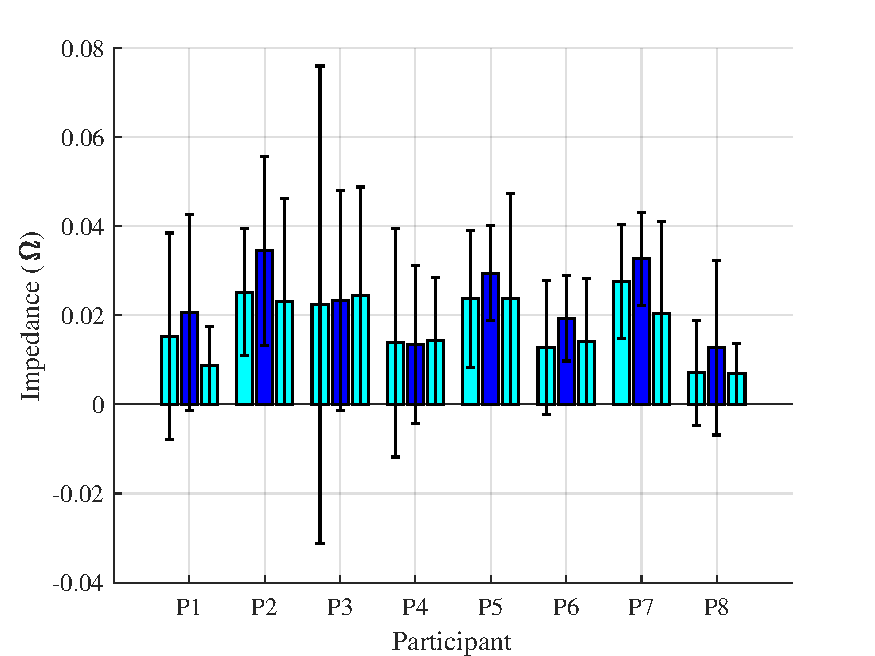
\includegraphics[height=6cm,keepaspectratio,keepaspectratio]{figure9b}    
		\caption{Change of amplitude of the waveform at point B}
		\label{fig:change_B_arterial}
	\end{subfigure}
	~
	\begin{subfigure}[t]{0.5\textwidth}
		\centering
		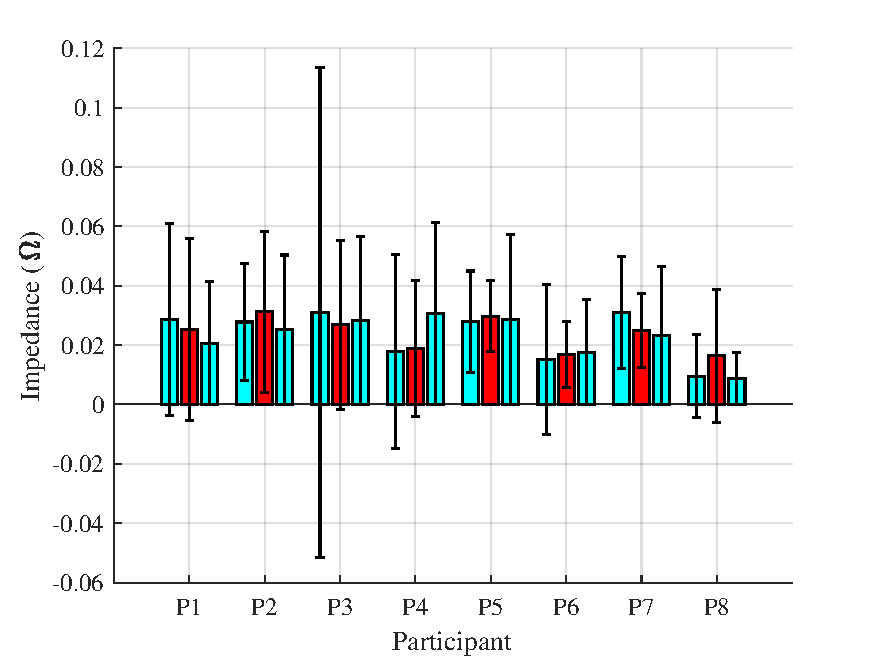
\includegraphics[height=6cm,keepaspectratio]{figure9c}    
		\caption{Change of amplitude of the waveform at point C}
		\label{fig:change_C_arterial}
	\end{subfigure}%
	\caption{Changes of the impedance peak values during baseline, partial arterial occlusion and return to baseline for points A,B and C.}
	\label{fig:iPG_change_points_arterial}
\end{figure*}

\subsubsection{Changes in systolic peak (Point A)}
\label{section results 3.2.1}
Through this occlusive event, six participants (\SI{75}{\percent}) experienced an increase in electrical resistivity in the point A. The average increase was about \SI{18.10}{\percent}.  On the other hand, the participants whose impedance decreased was in average \ SI {-6.77} {\ percent}. In general, it can be noticed the growth at this point. Figure \ref{fig:change_A_arterial} shows the change in amplitude for each one. Table \ref{tbl:change_A_arterial} summarises the average impedances and the changes in each region. 

After the cuff was deflated, the peak impedance of most of the participants (\SI{75}{\percent})  decreased in mean \SI{-21.13}{\percent}).  In contrast, participants three and four showed an increase in impedance of \SI{12.71}{\percent} and \SI{107.91}{\percent}. A large number of the latter being compared to its standard deviation shows that there must be noise in the signal affecting its quality.   

\begin{table}[!htbp]
	\caption{Change of amplitude of the waveform at peak A during the transition from baseline to venous occlusion.}
	\label{tbl:change_A_arterial}
	\centering\small
	\begin{tabular}{l
			*{3}{S[table-format=1.4]@{\,\( \pm \)\,}S[table-format=1.4]} %Format for Z+-std
			cc}
		\toprule
		& \multicolumn{2}{c}{\multirow{2}{*}{\textbf{Baseline [\si{\ohm}]}}}
		& \multicolumn{2}{c}{\multirow{2}{*}{\textbf{Occlusion [\si{\ohm}]}}}
		& \multicolumn{2}{c}{\multirow{2}{*}{\textbf{Baseline [\si{\ohm}]}}}
		& \multicolumn{2}{c}{\textbf{Change}} \\
		& \multicolumn{2}{c}{}
		& \multicolumn{2}{c}{}
		& \multicolumn{2}{c}{}
		&\textbf{R1-R2}&\textbf{R2-R3}\\\midrule
		Participant 1    &     0.0305    &     0.0194    &     0.0275    &     0.0190    &     0.0265    &     0.0265    &     -9.73    \%      &      -3.30    \%      \\  
		Participant 2    &     0.0449    &     0.0140    &     0.0497    &     0.0197    &     0.0461    &     0.0461    &     10.74    \%      &      -8.02    \%      \\  
		Participant 3    &     0.0294    &     0.0379    &     0.0307    &     0.0185    &     0.0356    &     0.0356    &      4.11    \%      &      16.71    \%      \\  
		Participant 4    &     0.0222    &     0.0242    &     0.0214    &     0.0152    &     0.0453    &     0.0453    &     -3.81    \%      &     107.91    \%      \\  
		Participant 5    &     0.0376    &     0.0133    &     0.0433    &     0.0115    &     0.0351    &     0.0351    &     15.30    \%      &     -21.83    \%      \\  
		Participant 6    &     0.0251    &     0.0096    &     0.0272    &     0.0081    &     0.0251    &     0.0251    &      8.30    \%      &      -8.36    \%      \\  
		Participant 7    &     0.0365    &     0.0097    &     0.0525    &     0.0092    &     0.0394    &     0.0394    &     43.53    \%      &     -35.69    \%      \\  
		Participant 8    &     0.0127    &     0.0104    &     0.0161    &     0.0160    &     0.0098    &     0.0098    &     26.65    \%      &     -49.61    \%      \\      
		\bottomrule
	\end{tabular} 
\end{table}\subsubsection{Changes in dicrotic notch peak (Point B)}
\label{section results 3.2.2}
In the dicrotic notch position (point B), there was a similar trend as the one seen in the systolic peak. In total, seven out of eight participants registered an increase of impedance. The average increase at the dicrotic notch was about \SI{35.52}{\percent}. Only participant four showed a  slight drop in impedance (\SI{-2.44}{\percent}).  

When the pressure was removed, six out of eight of the study members experience a fall in electrical resistivity. In averaged, it reduced \SI{-52.39}{\percent}. Again, participant four was the exception to this reduction, as well as participant three. Their impedance rose \SI{5.72}{\percent} and \SI{4.61}{\percent}.

Figure \ref{fig:change_B_arterial} evidences these changes in each region. Table \ref{fig:change_B_arterial} details the mean impedances and the ratio of change between each region.

\begin{table}[!htbp]
	\caption{Change of amplitude of the waveform at peak B during the transition from baseline to venous occlusion.}
	\label{tbl:change_B_arterial}
	\centering\small
	\begin{tabular}{l
			*{3}{S[table-format=1.4]@{\,\( \pm \)\,}S[table-format=1.4]} %Format for Z+-std
			cc}
		\toprule
		& \multicolumn{2}{c}{\multirow{2}{*}{\textbf{Baseline [\si{\ohm}]}}}
		& \multicolumn{2}{c}{\multirow{2}{*}{\textbf{Occlusion [\si{\ohm}]}}}
		& \multicolumn{2}{c}{\multirow{2}{*}{\textbf{Baseline [\si{\ohm}]}}}
		& \multicolumn{2}{c}{\textbf{Change}} \\
		& \multicolumn{2}{c}{}
		& \multicolumn{2}{c}{}
		& \multicolumn{2}{c}{}
		&\textbf{R1-R2}&\textbf{R2-R3}\\\midrule
		Participant 1    &     0.0153    &     0.0232    &     0.0206    &     0.0220    &     0.0087    &     0.0087    &     35.05    \%      &     -77.89    \%      \\  
		Participant 2    &     0.0252    &     0.0142    &     0.0345    &     0.0212    &     0.0231    &     0.0231    &     36.75    \%      &     -44.93    \%      \\  
		Participant 3    &     0.0224    &     0.0536    &     0.0234    &     0.0247    &     0.0244    &     0.0244    &      4.42    \%      &       4.61    \%      \\  
		Participant 4    &     0.0138    &     0.0256    &     0.0135    &     0.0177    &     0.0143    &     0.0143    &     -2.44    \%      &       5.72    \%      \\  
		Participant 5    &     0.0237    &     0.0155    &     0.0294    &     0.0107    &     0.0237    &     0.0237    &     24.19    \%      &     -24.13    \%      \\  
		Participant 6    &     0.0128    &     0.0150    &     0.0193    &     0.0096    &     0.0141    &     0.0141    &     50.42    \%      &     -40.66    \%      \\  
		Participant 7    &     0.0276    &     0.0128    &     0.0327    &     0.0104    &     0.0205    &     0.0205    &     18.66    \%      &     -44.28    \%      \\  
		Participant 8    &     0.0071    &     0.0118    &     0.0127    &     0.0196    &     0.0069    &     0.0069    &     79.15    \%      &     -82.44    \%      \\    
\bottomrule
	\end{tabular} 
\end{table}

\subsubsection{Changes in diastolic peak (Point C)}
\label{section results 3.2.3}
Changes in the diastolic peak also presented a similar trend as seen in points A and B. However; the changes were not as marked as the ones seen before. Figure \ref{fig:change_C_arterial} and Table \ref{tbl:change_C_arterial} summarise the values obtained. In total, \SI{62.5}{\percent} showed an increase of impedance between region 3 and 4. It increased with a median of \SI{21.68}{\percent}. Participant eight showed a change significantly larger than the mean (\SI{71.41}{\percent}). Others study members pointed a decrease of electrical resistivity in \SI{-14.71}{\percent} in average.  

On the opposite side of the exercise, after releasing the pressure, a similar number of partakers whose peak increased showed a reduction in impedance (\SI{62.5}{\percent}).  However, these were different members. In average, impedance reduced \SI{-25.56}{\percent} in total. Again, participant eight showed a greater ratio of change significantly exceeding the mean. On the other hand, participants that exhibited an increase of impedance, the average was \SI{25.23}{\percent}. Participant four outperformed notably the average ratio (\SI{66.03}{\percent}).

\begin{table}[!htbp]
	\caption{Change of amplitude of the waveform at peak C during the transition from baseline to venous occlusion.}
	\label{tbl:change_C_arterial}
	\centering\small
	\begin{tabular}{l
			*{3}{S[table-format=1.4]@{\,\( \pm \)\,}S[table-format=1.4]} %Format for Z+-std
			cc}
		\toprule
		& \multicolumn{2}{c}{\multirow{2}{*}{\textbf{Baseline [\si{\ohm}]}}}
		& \multicolumn{2}{c}{\multirow{2}{*}{\textbf{Occlusion [\si{\ohm}]}}}
		& \multicolumn{2}{c}{\multirow{2}{*}{\textbf{Baseline [\si{\ohm}]}}}
		& \multicolumn{2}{c}{\textbf{Change}} \\
		& \multicolumn{2}{c}{}
		& \multicolumn{2}{c}{}
		& \multicolumn{2}{c}{}
		&\textbf{R1-R2}&\textbf{R2-R3}\\\midrule
		Participant 1    &     0.0286    &     0.0323    &     0.0253    &     0.0307    &     0.0206    &     0.0206    &     -11.44    \%      &     -16.31    \%      \\  
		Participant 2    &     0.0278    &     0.0196    &     0.0312    &     0.0272    &     0.0252    &     0.0252    &      12.45    \%      &     -21.78    \%      \\  
		Participant 3    &     0.0310    &     0.0826    &     0.0268    &     0.0284    &     0.0283    &     0.0283    &     -13.49    \%      &       4.71    \%      \\  
		Participant 4    &     0.0178    &     0.0327    &     0.0189    &     0.0229    &     0.0306    &     0.0306    &       5.94    \%      &      66.03    \%      \\  
		Participant 5    &     0.0279    &     0.0171    &     0.0298    &     0.0119    &     0.0287    &     0.0287    &       6.74    \%      &      -3.96    \%      \\  
		Participant 6    &     0.0151    &     0.0252    &     0.0169    &     0.0111    &     0.0176    &     0.0176    &      11.86    \%      &       4.96    \%      \\  
		Participant 7    &     0.0309    &     0.0189    &     0.0249    &     0.0124    &     0.0232    &     0.0232    &     -19.19    \%      &      -5.65    \%      \\  
		Participant 8    &     0.0096    &     0.0139    &     0.0164    &     0.0224    &     0.0087    &     0.0087    &      71.41    \%      &     -80.09    \%      \\  

		\bottomrule
	\end{tabular} 
\end{table}

\subsection{Plethysmography waveform change during total occlusion}
\label{section results 3.3}
Performing total occlusion completely blocks the inflow and outflow of blood beneath the arm's cuff.  Hence, there is no change of volume within the arm's segment. As a result, impedance plethysmography should not present changes.  Figure \ref{fig:iPG_total} shows the plethysmography baseline in region 5 (\SIrange{960}{1260}{\second}) and region 6  (\SIrange{1260}{1440}{\second}) of participant seven. As portrayed by the Figure \ref{fig:iPG_change_points_total}, the amplitudes of most of the participants dropped during the occlusion.

However, participant four experience different behaviour in all the points. The standard deviation of this participant also suggests that there would have been a problem with his plethysmography signal during the test. 

In general, point A decreased in average \SI{-66.15}{\percent} its peak value occlusion. Then when the pressure was released, impedance recovered its value in \SI{75.98}{\percent}. A similar event occurred with point B; peak signals dropped a median of \SI{-63.29}{\percent} during blockage and recovered in average to \SI{74.02}{\percent}. Alike, point C, decreased in average \SI{-50.27}{\percent}  and increased \SI{58.71}{\percent} after the occlusion.

\begin{figure*}[!htbp]
	\centering
	\begin{subfigure}[t]{0.5\textwidth}
		\centering
		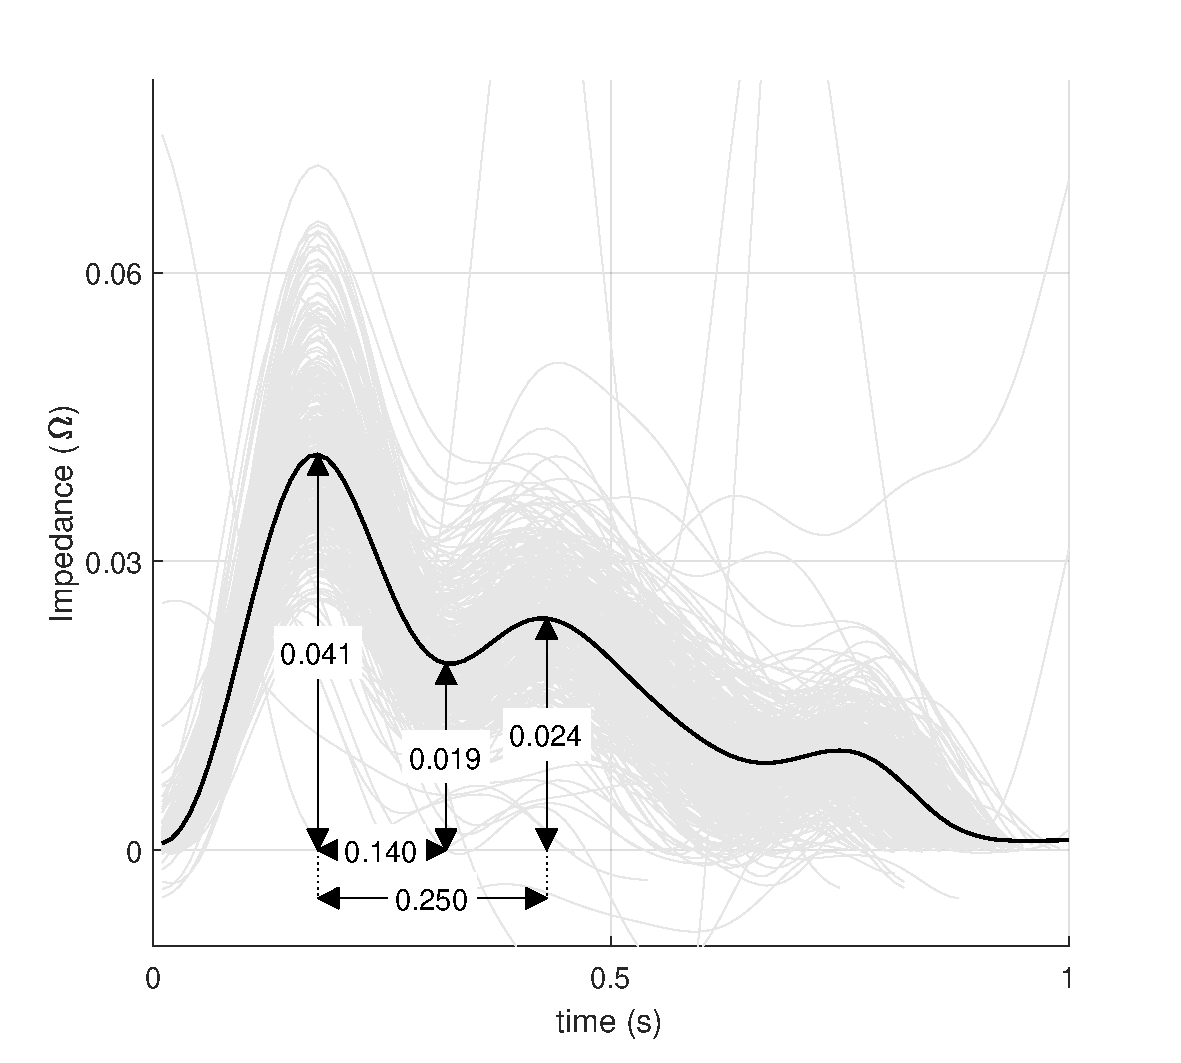
\includegraphics[height=7.6cm]{figure10a}
		\caption{Average plethysmography waveform during venous occlusion region 5 (\SIrange{960}{1260}{\second})}
		\label{fig:iPG_total_baseline}
	\end{subfigure}%
	~ 
	\begin{subfigure}[t]{0.5\textwidth}
		\centering
		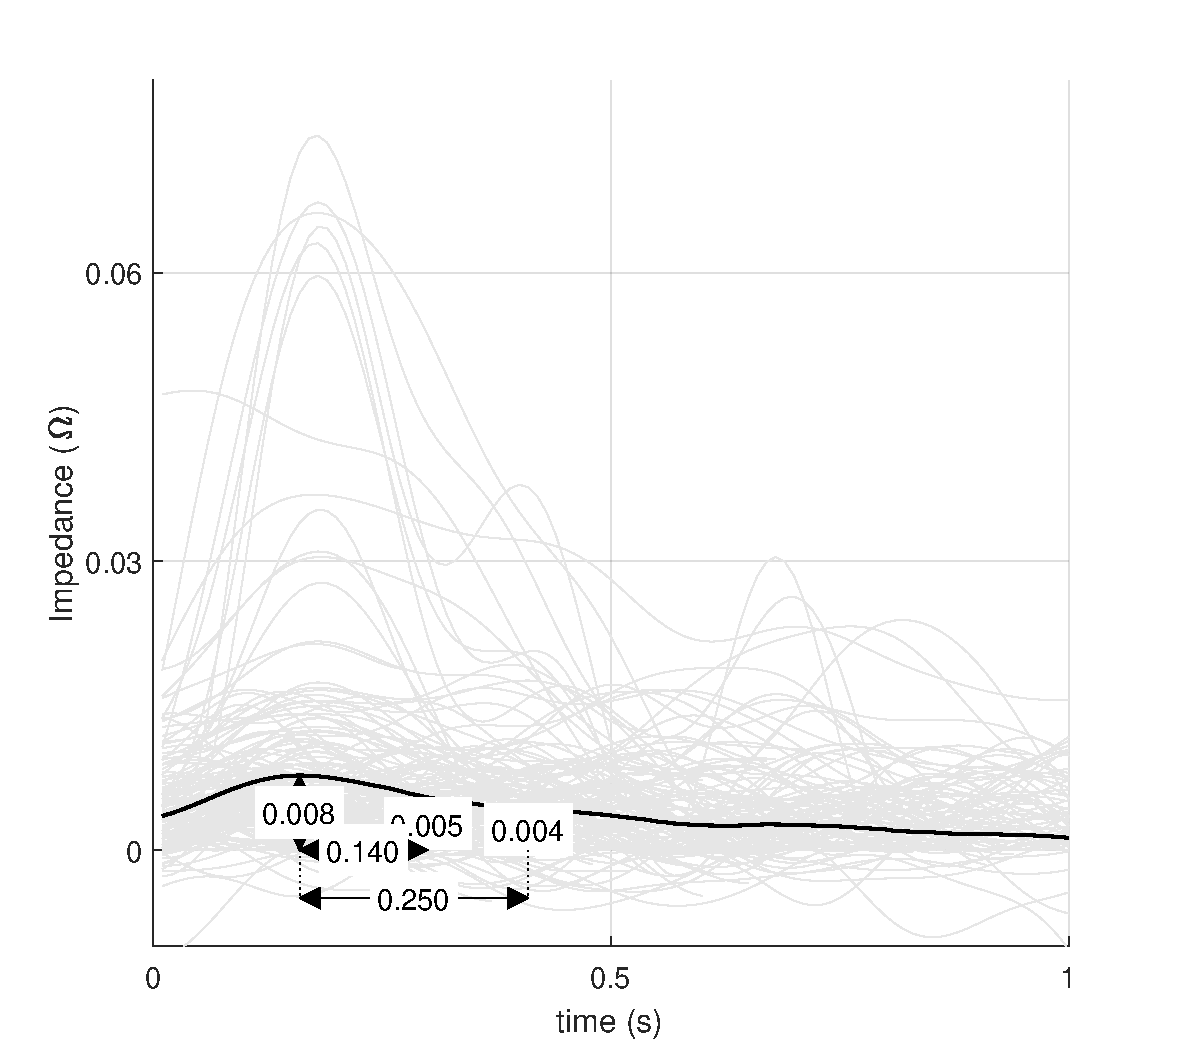
\includegraphics[height=7.6cm]{figure10b}
		\caption{Average plethysmography waveform during venous occlusion region 6 (\SIrange{1260}{1440}{\second})}
		\label{fig:iPG_total_occlusion}
	\end{subfigure}
	\caption{Plethysmography waveform of the participant seven between baseline and total occlusion}
	\label{fig:iPG_total}
\end{figure*}

\begin{figure*}[!htbp]
	\centering
	\begin{subfigure}[t]{0.5\textwidth}
		\centering
		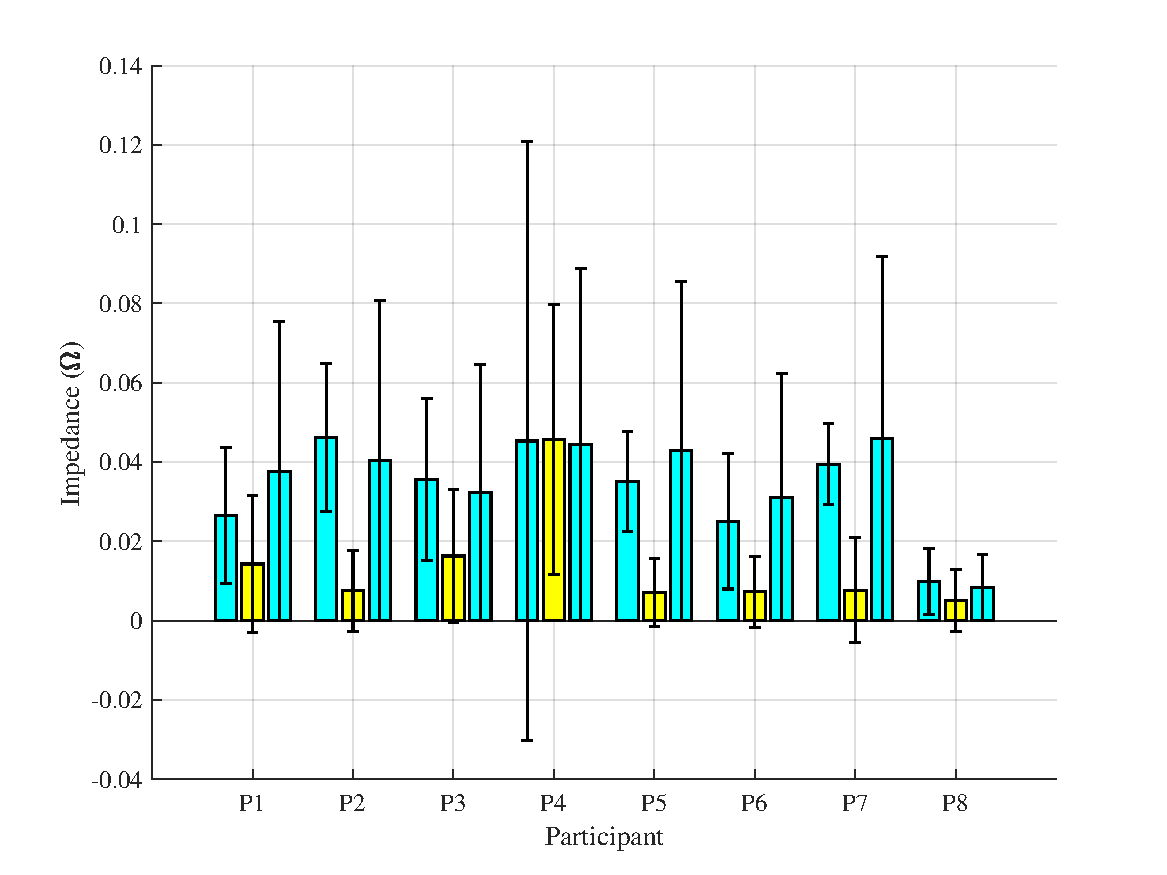
\includegraphics[height=6cm,keepaspectratio]{figure11a}    
		\caption{Change of amplitude of the waveform at point A.}
		\label{fig:change_A_total}
	\end{subfigure}%
	~ 
	\begin{subfigure}[t]{0.5\textwidth}
		\centering
		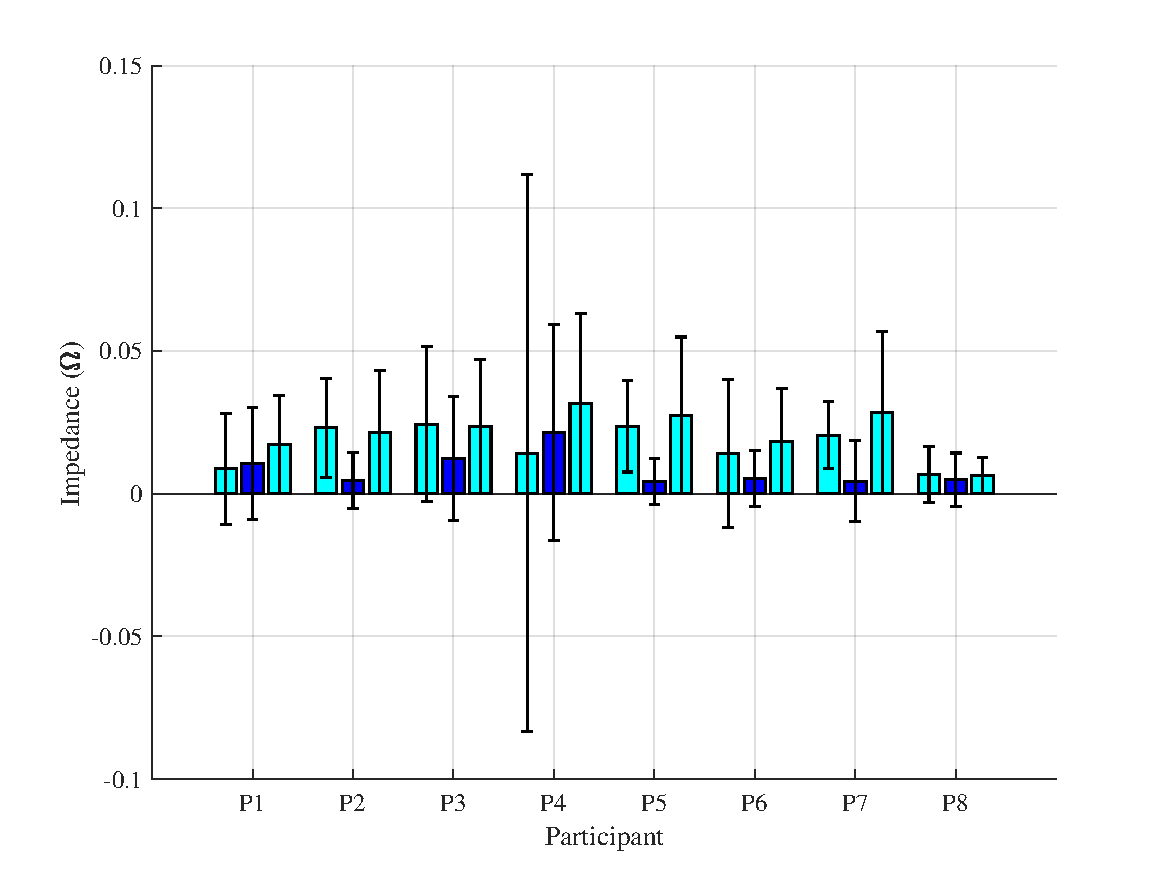
\includegraphics[height=6cm,keepaspectratio]{figure11b}    
		\caption{Change of amplitude of the waveform at point B}
		\label{fig:change_B_total}
	\end{subfigure}
	~
	\begin{subfigure}[t]{0.5\textwidth}
		\centering
		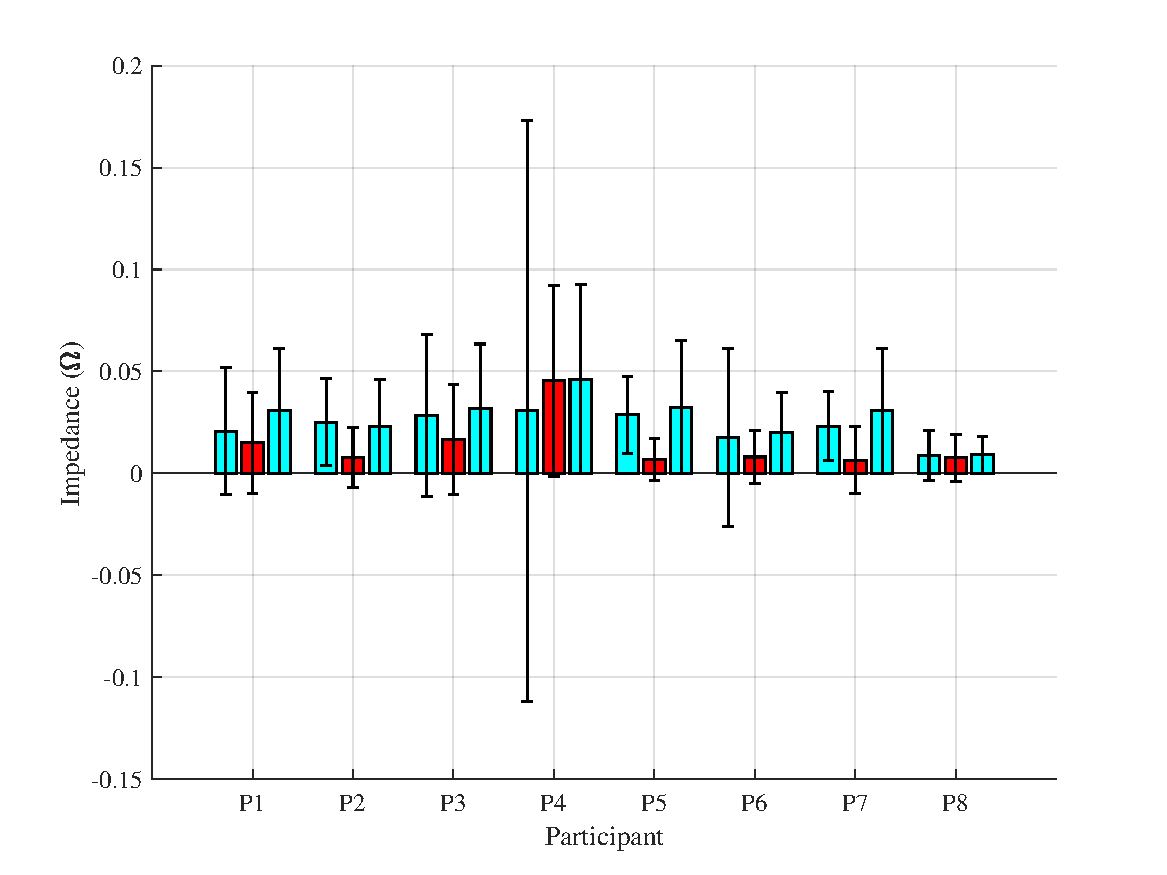
\includegraphics[height=6cm,keepaspectratio]{figure11c}    
		\caption{Change of amplitude of the waveform at point C}
		\label{fig:change_C_total}
	\end{subfigure}%
	\caption{Changes of the impedance peak values during baseline, total occlusion and return to baseline for points A,B and C.}
	\label{fig:iPG_change_points_total}
\end{figure*}


%%********************************** % Section 5.4 ******************************************
\pagebreak
\section{Blood flow calculation from baseline signal}
\label{section results 4}

%********************************** % Section 5.4.1 ******************************************
\subsection{Blood flow calculation using venous occlusion plethysmography}
\label{section results 4.1}
Using the method venous occlusion plethysmography is possible to calculate the blood flow in the forearm segment. As it can be seen from figure \ref{fig:blood_flow:venous_occlusion} the data is not dropping in a completely straight line. As a reminder, the occlusion occurred during \SIrange{300}{480}{\second} which is the time lapse showed. There are impedance variations caused by respiration movement contained within the signals, but also some sections are affected by muscle contraction. If the blood flow were computed using point by point method, there would be some discrepancies when the resistivity is increasing. Thus, this will lead to an incorrect reflection of the blood stream. 

As a result, the method described in section xxx was used to calculate the blood flow between decreasing points only. In short, this algorithm finds the peak and valleys of the signal and then computes the blood flow using equation \ref{eq:QL} between those points found. The figure \ref{fig:blood_flow:venous_occlusion} on the left shows the impedance decrease during the occlusion for all participants. The image on also depicts the points from where the algorithm extracted the reference points for its calculations. In this case, the red triangle pointing downwards is equivalent to the base impedance $R_B$ and the black triangle is the ending point of the calculation point. Then $\Delta R / \Delta t$ can be obtained as the difference between these two points in impedance and time. 
\mynote{Add a section describing how the data was treated.} 

In the same figure but on the right, it can be noticed the result of the blood flow calculated in units of \si{\bfv}. The blue dots indicate the instant blood flow at the end value of $\Delta R$. The orange line indicates the mean blood flow during measurements. Again, participants 1 and 6 flow estimation is affected by movement producing a mean value far from the majority of the data points. Moreover, it is confirmed by examining the results summarised on the table \ref{tbl:blood_flow:region2}. The standard deviation $(\sigma_x)$ is quite far compared to the rest of the participants, as well as the minimum value of the data. Therefore, the results of these two participants clearly cannot be expected to be accurate. However, if the data sample was in a linear section, then the calculated flow will be more in agreement with the expected values. 

From this table can be noticed that the calculated blood flow per \SI{100}{\ml} of tissue for all the participants was in average \flowbasalvenous{}. 

\begin{table}[t]
	\caption{Statistics of the blood flow calculated during venous occlusion. All the numbers are in blood flow units \si{\bfv}, except the column size that is the magnitude of sample.}
	\label{tbl:blood_flow:region2}
	\centering
	\begin{tabular}
		{
			l
			c
			c
			S[table-format=1.3]@{\,\( \pm \)\,}S[table-format=1.3] %Format for Z+-std 
			c
			c
		}
		\toprule
		& \multirow{2}{*}{\textbf{Size}} 
		& \textbf{Median} 
		& \multicolumn{2}{c}{\textbf{Mean}} 
		& \textbf{Max} & \textbf{Min} \\
		& 
		& \small{\si{[\bfv]}} 
		& \multicolumn{2}{c}{\small{\si{[\bfv]}}} 
		& \small{\si{[\bfv]}} 
		& \small{\si{[\bfv]}} \\\midrule
		Participant 1   & 23   &     -0.808  &   -1.055  &  0.939 &   -0.054   &  -3.955\\
		Participant 2   & 30   &     -0.570  &  -0.575   & 0.272  &  -0.117    & -1.256\\
		Participant 3   & 31   &     -0.600  &  -0.613   & 0.344  &  -0.011    & -1.483\\
		Participant 4   & 34   &     -1.131  &  -1.146   & 0.720  &  -0.016    & -2.979\\
		Participant 5   & 23   &     -0.606  &  -0.611   & 0.345  &  -0.062    & -1.737\\
		Participant 6   & 29   &     -0.710  &  -1.510   & 2.639  &  -0.092    &-10.865\\
		Participant 7   & 25   &     -0.575  &  -0.613   & 0.284  &  -0.025    & -1.141\\
		Participant 8   & 42   &     -0.605  &  -0.716   & 0.530  &  -0.072    & -2.743\\ \bottomrule
	\end{tabular} 
\end{table}

\begin{figure}
	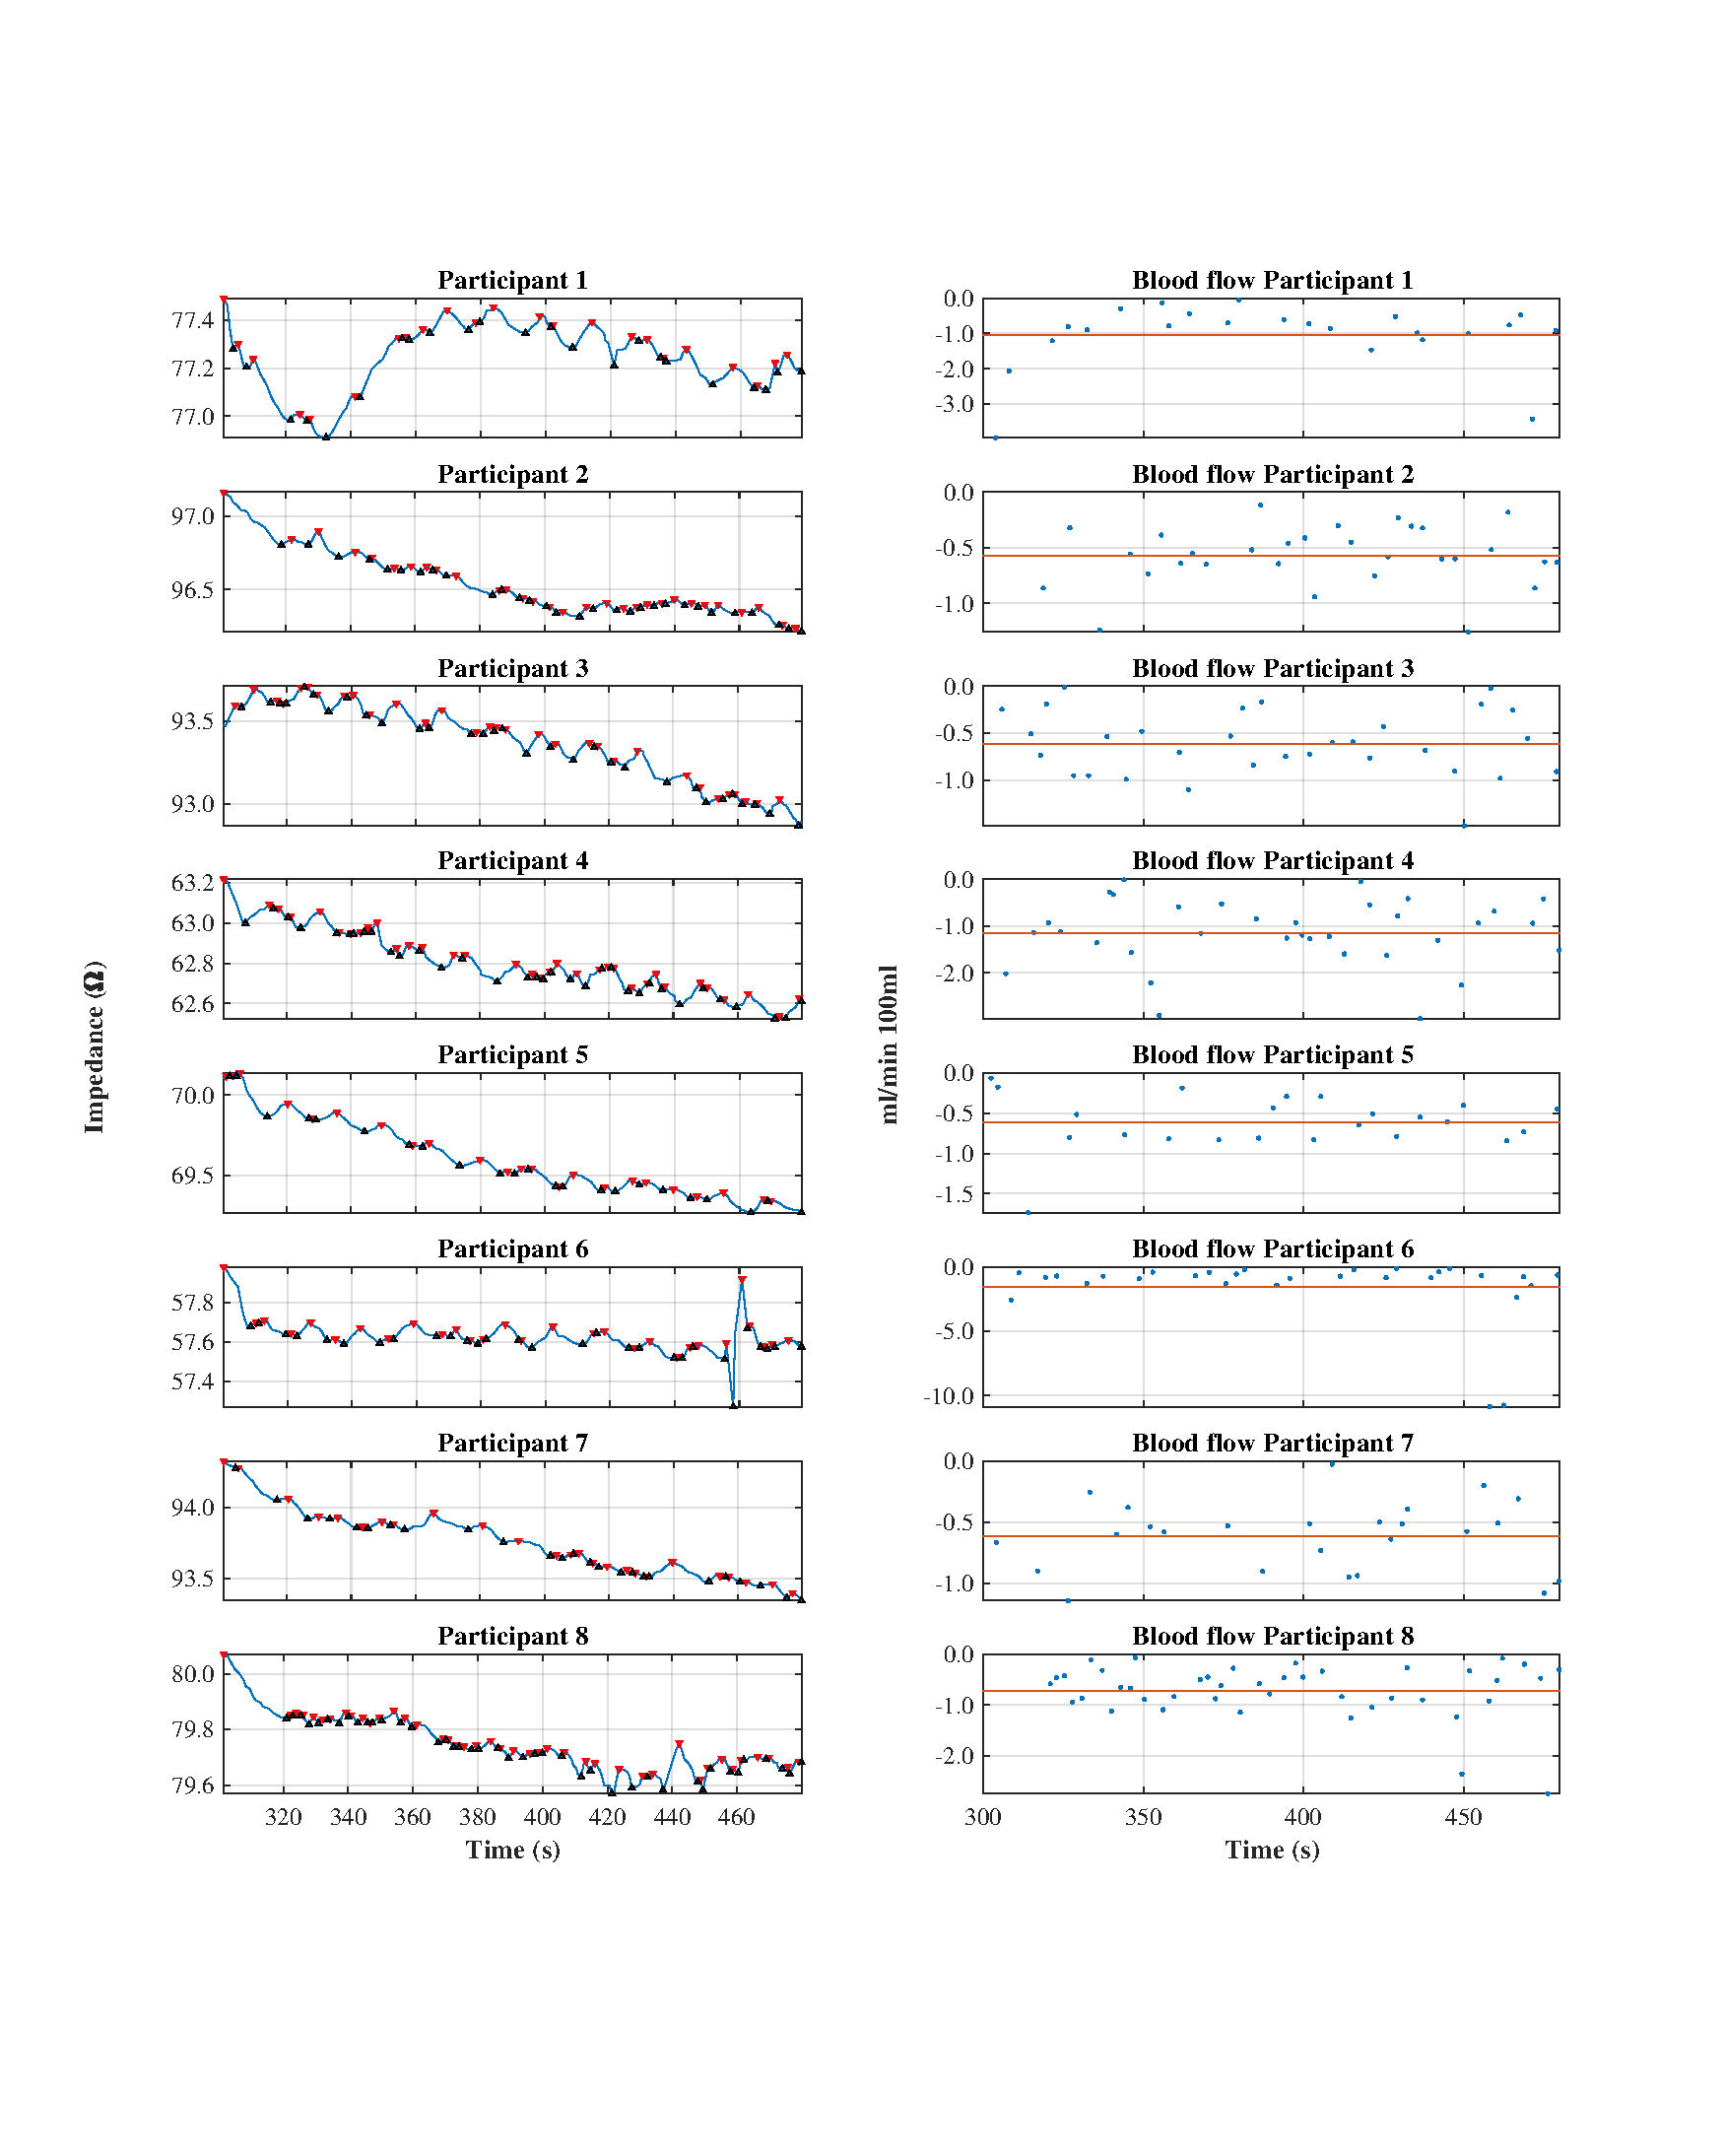
\includegraphics[width=\textwidth,height=\textheight,keepaspectratio,trim={0.5cm 0.5cm 2cm 2cm},clip]{figure12}    
	\caption{Blood flow calculated from venous occlusion plethysmography}
	\label{fig:blood_flow:venous_occlusion}
\end{figure}

%********************************** % Section 5.4.2 ******************************************
\subsection{Blood flow calculation during partial arterial occlusion}
\label{section results 4.2}
As reflected in \ref{section results 2.2}, there is a deeper slope in basal impedance during partial arterial occlusion compared to venous obstruction. Therefore, higher blood flow values are expected from the calculated data. The method used to estimate the blow was the same one utilised in the section \ref{section results 4.1}. The obtained signals were also affected by noise within the basal impedance, possibly caused by the respiratory action and muscle movement. In fact, during this part of the experiment, most participants felt uncomfortable feeling numbness in their arms. Therefore, they moved their arms during this section of the investigation which in part affected the quantification of blood flow.

The figure \ref{fig:blood_flow:arterial_occlusion} shows the calculation of the blood flow between the points of decreasing impedance. From a qualitative perspective, it can be observed that some signals do not show a decreasing linear trend. For example, participant 1 at the end of the test abruptly moved his arm causing a sudden change in impedance. As a result, the impedance at this point was far from the mean of the signal.

Another example of unexpected impedance change is the participant 4 and 8. In the first case, in the middle of the test, the impedance of the forearm tended to increase. However, this later began to decline as expected. In the second case, the movement of the arm can be observed after half of the test. As a result, there was a rapid acceleration of blood flow that is not in agreement with the average value of the signal.

By analysing the results summarised in the Table \ref{tbl:blood_flow:region4} the average blood flow of all the participants was \flowbasalarterial{}. In general, there was an increment of \SI{9.52}{\percent} compared to venous occlusion. 


\begin{table}[h]
	\caption{Statistics of the blood flow calculated during partial arterial occlusion. All the numbers are in blood flow units \si{\bfv}, except the column size that is the magnitude of sample.}
	\label{tbl:blood_flow:region4}
	\centering
	\begin{tabular}
		{
			l
			c
			c
			S[table-format=1.3]@{\,\( \pm \)\,}S[table-format=1.3] %Format for Z+-std 
			c
			c
		}
		\toprule
		& \multirow{2}{*}{\textbf{Size}} 
		& \textbf{Median} 
		& \multicolumn{2}{c}{\textbf{Mean}} 
		& \textbf{Max} & \textbf{Min} \\
		& 
		& \small{\si{[\bfv]}} 
		& \multicolumn{2}{c}{\small{\si{[\bfv]}}} 
		& \small{\si{[\bfv]}} 
		& \small{\si{[\bfv]}} \\\midrule
		Participant 1    &      24        &      -0.917    &      -1.118    &      1.090    &      -0.105    &      -5.238    \\ 
		Participant 2    &      27        &      -0.632    &      -0.950    &      0.996    &      -0.014    &      -4.821    \\ 
		Participant 3    &      27        &      -0.778    &      -0.966    &      0.736    &      -0.087    &      -3.546    \\ 
		Participant 4    &      35        &      -0.803    &      -1.184    &      1.129    &      -0.013    &      -5.462    \\ 
		Participant 5    &      22        &      -0.793    &      -0.725    &      0.292    &      -0.199    &      -1.250    \\ 
		Participant 6    &      28        &      -0.885    &      -0.952    &      0.695    &      -0.114    &      -2.628    \\ 
		Participant 7    &      25        &      -0.496    &      -0.524    &      0.350    &      -0.031    &      -1.498    \\ 
		Participant 8    &      26        &      -0.743    &      -1.141    &      1.170    &      -0.042    &      -4.708    \\ 
\bottomrule
	\end{tabular} 
\end{table}

\begin{figure}
	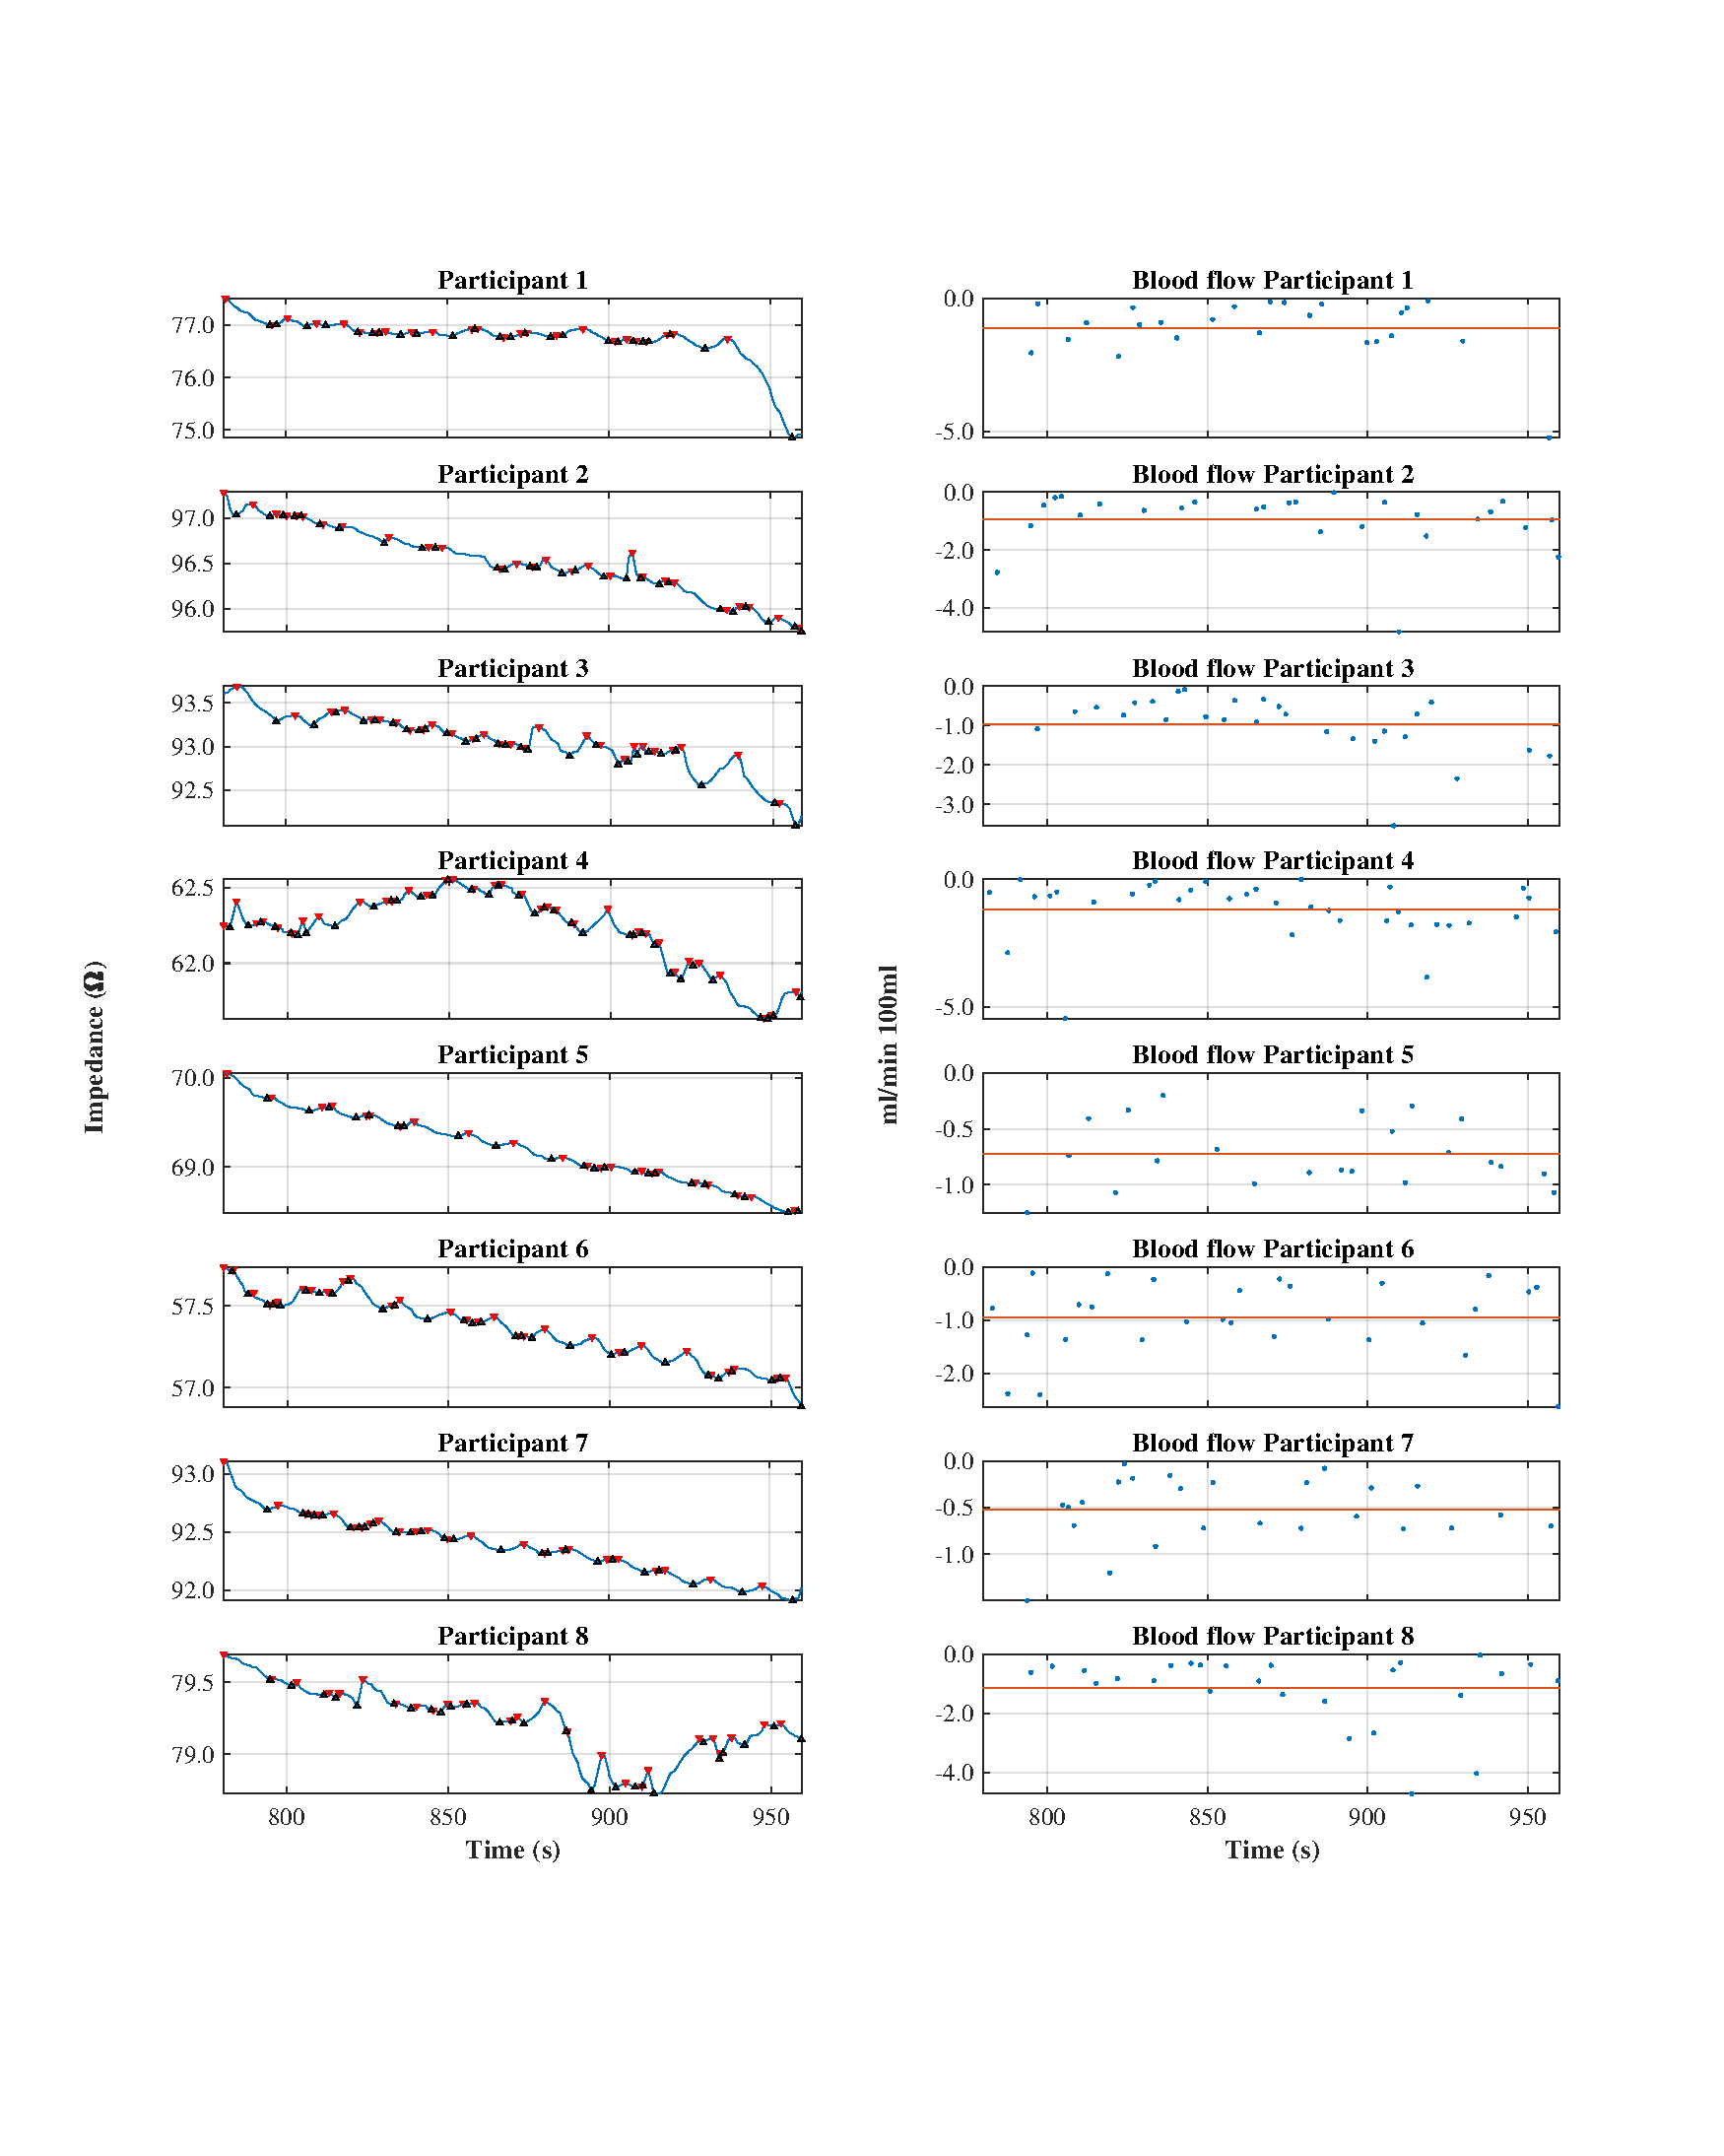
\includegraphics[width=\textwidth,height=\textheight,keepaspectratio,trim={0.5cm 0.5cm 2cm 2cm},clip]{figure13}    
	\caption{Blood flow calculated from partial arterial occlusion plethysmography}
	\label{fig:blood_flow:arterial_occlusion}
\end{figure}

%%********************************** % Section 5.4.3 ******************************************
\subsection{Comparative change of blood flow between venous and partial arterial}
\label{section results 4.3}
As it can be noticed from Figure \ref{fig:iPG_flow_comparative}, the quantitative analysis of blood flow change between venous occlusion and partial arterial occlusion shows a tendency to increase flow. The negative symbol of the data was suppressed in the figure since it expresses direction only. 

The graph is divided into two parts, one from the average value and another from the median of the data.  In both situations \SI{75}{\percent} of the participants showed an increase in their blood flow, but only member 7 was common in both charts. This participant oddly showed a decrease in his mean and median value, which is utterly inexplicable at this time since his signals are quite constant. Though from figure \ref{fig:rb:all_participants} can be noticed that from the beginning of the session to the end of the partial arterial occlusion  (\SIrange{0}{960}{\second}), his basal impedance was declining continuously, but after this time it followed a downtrend. 

On the other hand, it appears that the median value of participant 6 was heavily affected by a sudden change of the basal impedance signal towards the end of the test in venous occlusion. In fact, As table \ref{tbl:blood_flow:region2} shows there are extremely high values in the blood flow up to (\SI{10}{\bfv}, this clearly was caused by movement effect. 

Participant 4 is another interesting case, as it has been detailed in this document, the partaker exhibited unusual changes during the experiment. In this case, the median of the signal showed a decrease in blood flow.However, this can be explained by the shape of the basal impedance signal illustrated in figure \ref{fig:blood_flow:arterial_occlusion}. As can be seen, the signal does not contain many points with a very steep negative slope, and this reflects small changes in impedance, which also translates into a low value in the blood stream which might be incorrect. By looking at the same graph but the blood flow plot, from \SIrange{760}{870}{\second} the blood flow is quite small but after that period values tend to be more in agreement.

\begin{figure*}[!htbp]
	\centering
	\begin{subfigure}[t]{0.5\textwidth}
		\centering
		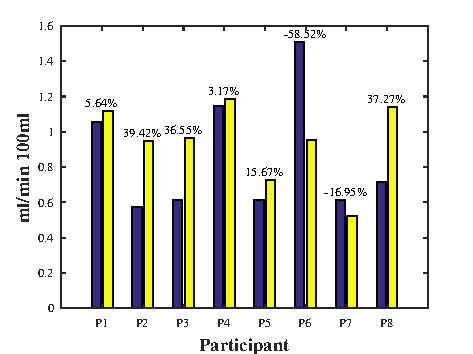
\includegraphics[height=6cm,keepaspectratio]{figure14a}    
		\caption{Comparison between mean venous occlusion and partial arterial occlusion. Ration of change showed as a percentage.}
		\label{fig:change_flow_mean}
	\end{subfigure}%
	~ 
	\begin{subfigure}[t]{0.5\textwidth}
		\centering
		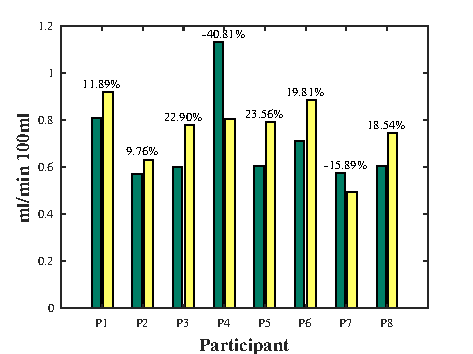
\includegraphics[height=6cm,keepaspectratio,keepaspectratio]{figure14b}    
		\caption{Comparison between median venous occlusion and partial arterial occlusion. Ration of change showed as a percentage.}
		\label{fig:change_flow_median}
	\end{subfigure}
	\caption{Change of blood flow between venous occlusion and partial arterial occlusion}
	\label{fig:iPG_flow_comparative}
\end{figure*}


%%********************************** % Section 5.5 ******************************************
\section{Blood flow calculation from plethysmography signal}
\label{section results 5}
So far the blood flow has been analysed from occlusive methods using the techniques described in section \ref{section results 4}. However, these procedures require mechanical occlusion to produce an increase in volume within the forearm being measured. However, sometimes this can be uncomfortable especially when the applied pressure is above the systolic value or when the person simply can not tolerate restriction of blood flow.

For this cases, analysing the waveform also provides information about the blood flow.  The rush of blood into the vessel creates a small increase in volume within the limit of the potential electrodes which can be translated into the blood flow. Having, a device sensitive enough to detect this changes is crucial to provide an accurate estimation of the blood speed. As described in section \ref{section results 3}, the waveform contained within the basal impedance was amplified by the device achieving great detail. 

In fact, several studies \mynote{Add a reference to a study about AC blood flow estimation} have demonstrated that is possible to calculate blood flow from the plethysmography waveform. In this case, the change of impedance used to perform this calculation occurs between the foot of the wave and the systolic peak. This $\Delta Z$ is used to calculate blood flow by also applying Nyober's equation \ref{eq:Nyober}. 

Figure \ref{fig:blood_flow_plethysmography} shows the blood flow calculated from the amplitude of the systolic peak throughout the experimental session. Green dots show blood flow measurements during reference readings (regions 1, 3, 5 and 6). The other colours show venous occlusion in blue, partial arterial occlusion in red and total obstruction in grey. The dark line drawn above the signals corresponds to the calculation of the sixth-order polynomial fit during each measurement event. Overseeing the amplitude transition in each region will help understand how the flow changes with each occlusive event. The blood flow shown in the same figure does not include the negative sign which represents the direction of flow relative to the potential electrodes.

\begin{figure}[!htb]
	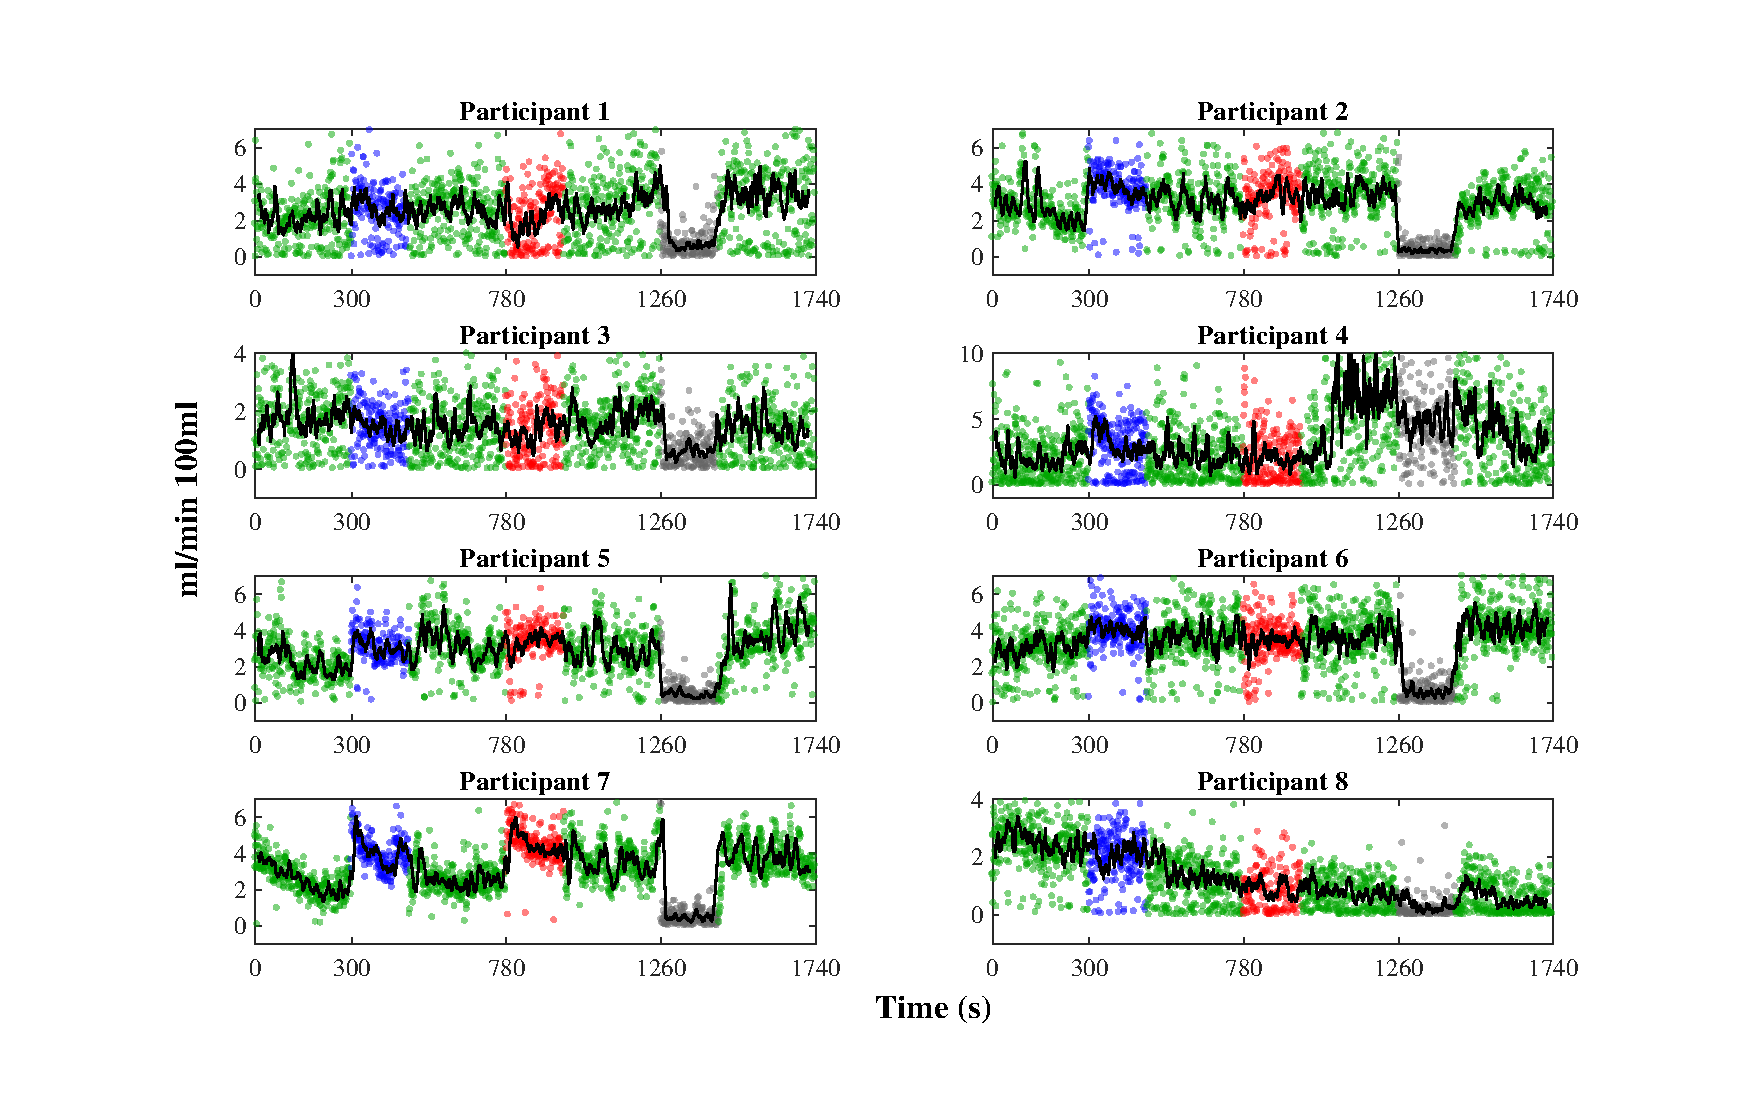
\includegraphics[width=\textwidth,keepaspectratio,trim={3cm 0cm 3cm 0 cm},clip]{figure15}    
	\caption[Blood flow calculated from impedance plethysmography waveform at the time of the whole expetiment]{Blood flow calculated for all the participants during the experiment. Each dot represents the peak value of the waveform that has been converted into flow (\si{\bfv}). The green dotted area represent the baselines measurements (regions 1,3,5 and 7). The region 2 (venous occlusion) is represented by the blue dots, arterial occlusions (region 4) are in red and total occlusions (region 6) are in grey.}
	\label{fig:blood_flow_plethysmography}
\end{figure}

As can be seen in the figure, between each transition in the middle of baseline and occlusion, there is a change in the calculated flow. In most participants, the change between baseline and venous occlusion creates a blood surge followed by a tendency for the flow to stabilise. It is worth noting that the addition of blood flow in participant 2 occurred before the occlusion. The reason for this is that the obstruction probably started before \SI{300}{\second} and the pressure applied to the arm was rather slow. There are other cases where the flow change occurred so fast that an entirely blank space can be seen connecting both events, as in participants 5 and 7. This situation, opposite to participant 2, was more likely that the cuff was inflated faster which did not allow a gradual but sudden change in flow. Finally, participant 8 is an exception to this rule. This participant experienced a decrease in flow, followed by a recovery and, he did not show a flow surge.

Between venous occlusion and baseline in region 3, the cuff was rapidly deflated to return blood flow to normal. However, from the calculated data it can be seen that there are no extreme changes in blood flow between these two sections. As it can be noticed, in most participants except partaker 1, there are small gaps between these two sections indicating that there is a slight change in blood flow. This action can be linked to a hyperaemic effect where as soon as the pressure of the cuff is released, the blood contained within the vessels of the forearm runs out to the upper part of the arm. After that, the blood flow tended to stabilise towards an average value. 

Similarly, as between regions 1 and 2, the change between baseline (region 3) and partial arterial occlusion (region 4) generated alterations in the calculated blood flow. Some participants also showed a rapid increase in blood flow followed by settling in the blood velocity. The only ones that did not enact a similar behaviour were participants 2 and 8. However,  partaker 7 appears to be Gaussian bell-shaped flow, which seems to indicate that the occlusion did not occur at the right moment but rather a little while later. Interestingly, the figure also shows that blood flow did not fully stabilise in participants 1, 3 and 8.

The change between partial arterial occlusion and baseline had a similar effect as the one described for the release of pressure of venous blockage. Most of the participants showed a decrease in their blood flow, possibly caused by the hyperaemic effect. At this point can be noticed that participant 4 started to show random blood flow readings. 

Total occlusion had a response as expected in almost all participants. When the blood flow was completely stopped, it was anticipated that its calculated value could tend to zero. In this case, the device was able to detect these changes. The only exception was participant 4 who again showed random results. At this point, it was to be expected that something wrong was happening with his measurements. Then, when the tourniquet was released, the blood flow returned in an exponential form and then set to an average value. In this case, the hyperaemic effect is more visible. It is worth noting that participant 8 showed a decline in blood flow measurements towards the midpoint of the test. This event agrees, with the participant expressing not feeling very well at the end of the test. It may be coincidence, or maybe the device was able to detect these physiological changes in him.

It seems evident that there is a blood surge when an occlusion occurs. Subsequently, the blood flow tends to stabilise at an average value. When the blockage is released, it seems that in some cases the flow tends to decrease and in others, there is no apparent change. The following sections will show the results of the change in mean blood flow during each occlusive event.


%********************************** % Section 5.5.1 ******************************************
\subsection{Blood flow change during venous occlusion}
\label{sectio results 5.1}
The following are the results of calculating mean blood flow between the transitions of baseline, venous occlusion and return to reference signal. Again, the result of the calculation is the absolute value, dropping the negative sign. Table \ref{tbl:blood_flow_iPG_venous} shows the result obtained by flow measurement in the scale \si{\bfv}. The mean blood flow in the region 1 was about \SI{2.398(0378)}{\bfv}. When the cuff was inflated below diastolic value, the blood flow calculated in the region 2, there was an average blood flow step-up of about \SI{3.043(0378)}{\bfv}. It is easy to see that in general terms there was an increment in the blood flow during the occlusion. In fact, \SI{75}{\percent} of the participants experienced this increment of blood flow. Only, study members 3 and 8 showed a decrease in their blood flow during this transition. The latter is not a surprise, as it was noted before, all his recordings started to go downwards from the beginning of the test. Their blood flow decreased in average roughly \SI{0.356(0023)}{\bfv}.

Clearly, there is a blood flow decrement when the cuff's tension was released to return to baseline. Indeed, seven out of eight of the participants experienced a drop in their flow rate during this part of the experiment. The average blood flow for the region 3 was approximately \SI{2.459(0852)}{\bfv}. The only one who did not experience this change was participant 6 whose flow rate dropped \SI{-0.0101}{\bfv} which means that practically there was not change. 

\begin{table}[h]
	\caption{Mean blood flow calculated form the plethysmography wave for baseline, venous occlusion and return to baseline}
	\label{tbl:blood_flow_iPG_venous}
	\centering
	\begin{tabular}{l
				    *{3}{S[table-format=1.3]@{\,\( \pm \)\,}S[table-format=1.3]} %Format for Z+-std
					}
		\toprule
		& \multicolumn{2}{c}{\textbf{Region 1}}
		& \multicolumn{2}{c}{\textbf{Region 2}} 
		& \multicolumn{2}{c}{\textbf{Region 3}}  \\
		& \multicolumn{2}{c}{\small{\si{[\bfv]}}} 
		& \multicolumn{2}{c}{\small{\si{[\bfv]}}} 
		& \multicolumn{2}{c}{\small{\si{[\bfv]}}} \\\midrule
		Participant 1    &     2.206     &     1.772    &     2.695     &     1.638    &     2.528     &     1.481    \\  
		Participant 2    &     2.715     &     1.185    &     3.786     &     1.161    &     3.122     &     1.252    \\  
		Participant 3    &     1.809     &     1.282    &     1.469     &     0.796    &     1.376     &     1.260    \\  
		Participant 4    &     2.178     &     2.032    &     3.088     &     2.010    &     2.177     &     1.959    \\  
		Participant 5    &     2.227     &     1.082    &     3.132     &     0.947    &     3.142     &     1.277    \\  
		Participant 6    &     3.035     &     1.289    &     4.049     &     1.146    &     3.581     &     1.330    \\  
		Participant 7    &     2.579     &     0.930    &     4.057     &     0.924    &     2.567     &     0.827    \\  
		Participant 8    &     2.437     &     0.874    &     2.065     &     0.901    &     1.176     &     0.729    \\  
		\bottomrule
	\end{tabular}
\end{table}

%********************************** % Section 5.5.2 ******************************************
\subsection{Blood flow change during partial arterial occlusion}
\label{section results 5.2}
The change of blood flow between baseline and partial occlusion had not a common in all the study participants response as the one seen in the previous section. Their flow rate increased from an average of \SI{2.458(0852)}{\bfv} to a mean blood flow of \SI{2.649(1200)}{\bfv}. It is clear that the increase was not as notorious compared to that saw on the venous occlusion. Indeed, only three participants (2, 5 and 7) showed an increment in blood flow with a centre of \SI{0.774(0983)}{\bfv}. Especially, Participant 3 showed a particularly higher increase in blood flow than the others with a value of \SI{1.099}{\bfv}. On the other hand, the rest of the participants exhibited a small decrease in their blood flow of an average of \SI{-0.160(0101)}{\bfv}. 

When the upper arm pressure was released, most participants were expected to show a decline in their flow. Nevertheless, this was not the case. Clearly, three participants depicted a drop in the rate (5, 7 and 8 with an average of \SI{-0.541(0371)}{\bfv}). The rest of the study members showed an increase in their collected data. However, as previously described in this region, Participant 4 showed random values whose results will not be added up to the total mean in the following calculation. The midpoint increase in blood flow between the others was \SI{0.329(0205)}{\bfv}. At this stage, it is not possible to draw a clear conclusion of the change of blood flow when the arterial occlusion occurred. 

\begin{table}[h]
	\caption{Mean blood flow calculated form the plethysmography wave for baseline, partial arterial occlusion and return to baseline}
	\label{tbl:blood_flow_iPG_arterial}
	\centering
	\begin{tabular}{l
			*{3}{S[table-format=1.3]@{\,\( \pm \)\,}S[table-format=1.3]} %Format for Z+-std
		}
		\toprule
		& \multicolumn{2}{c}{\textbf{Region 3}}
		& \multicolumn{2}{c}{\textbf{Region 4}} 
		& \multicolumn{2}{c}{\textbf{Region 5}}  \\
		& \multicolumn{2}{c}{\small{\si{[\bfv]}}} 
		& \multicolumn{2}{c}{\small{\si{[\bfv]}}} 
		& \multicolumn{2}{c}{\small{\si{[\bfv]}}} \\\midrule
		Participant 1    &     2.528     &     1.481    &     2.255     &     1.689    &     2.853     &     1.791    \\  
		Participant 2    &     3.122     &     1.252    &     3.298     &     1.399    &     3.418     &     1.492    \\  
		Participant 3    &     1.376     &     1.260    &     1.336     &     1.025    &     1.700     &     1.132    \\  
		Participant 4    &     2.177     &     1.959    &     2.091     &     1.895    &     5.669     &     7.032    \\  
		Participant 5    &     3.142     &     1.277    &     3.380     &     0.994    &     2.885     &     1.225    \\  
		Participant 6    &     3.581     &     1.330    &     3.432     &     1.197    &     3.667     &     1.558    \\  
		Participant 7    &     2.567     &     0.827    &     4.476     &     1.001    &     3.543     &     1.050    \\  
		Participant 8    &     1.176     &     0.729    &     0.924     &     0.864    &     0.729     &     0.537    \\  
	\bottomrule
	\end{tabular}
\end{table}

%********************************** % Section 5.5.3 ******************************************
\subsection{Blood flow change during total occlusion}
\label{section results 5.3}
The results obtained from total occlusion were quite close to the expected values.  The majority of the study participants showed a decrease in blood circulation rate close to zero.  As is evident from table \ref{tbl:blood_flow_iPG_total}, almost all participants showed a large dropped in the blood flow measurement when the blockage was applied in region 6. One more time, Participant 4 displayed completely unusual response during the occlusion. The values obtained were in average \SI{0.599(0224)}{\bfv} discarding data from partaker 4. Clearly, the flow obtained did not reflect a zero blood flow. The calculated values correspond to the amplitude of the noise level captured by the device. 

\begin{table}[!htbp]
	\caption{Mean blood flow calculated form the plethysmography wave for baseline, total occlusion and return to normality}
	\label{tbl:blood_flow_iPG_total}
	\centering
	\begin{tabular}{l
			*{3}{S[table-format=1.3]@{\,\( \pm \)\,}S[table-format=1.3]} %Format for Z+-std
		}
		\toprule
		& \multicolumn{2}{c}{\textbf{Region 5}}
		& \multicolumn{2}{c}{\textbf{Region 6}} 
		& \multicolumn{2}{c}{\textbf{Region 7}}  \\
		& \multicolumn{2}{c}{\small{\si{[\bfv]}}} 
		& \multicolumn{2}{c}{\small{\si{[\bfv]}}} 
		& \multicolumn{2}{c}{\small{\si{[\bfv]}}} \\\midrule
		Participant 1    &     2.853     &     1.791    &     0.908     &     1.283    &     3.407     &     2.553    \\  
		Participant 2    &     3.418     &     1.492    &     0.448     &     0.698    &     2.833     &     1.179    \\  
		Participant 3    &     1.700     &     1.132    &     0.704     &     0.751    &     1.387     &     1.210    \\  
		Participant 4    &     5.669     &     7.032    &     4.657     &     2.868    &     3.829     &     4.128    \\  
		Participant 5    &     2.885     &     1.225    &     0.560     &     0.687    &     3.619     &     1.645    \\  
		Participant 6    &     3.667     &     1.558    &     0.759     &     1.190    &     4.086     &     1.489    \\  
		Participant 7    &     3.543     &     1.050    &     0.597     &     1.121    &     3.767     &     0.958    \\  
		Participant 8    &     0.729     &     0.537    &     0.218     &     0.449    &     0.592     &     0.567    \\  
		\bottomrule
	\end{tabular}
\end{table}

After the tourniquet had been withdrawn, the blood flow returned to baseline following an exponential shape in most of the participants as shown in figure \ref{fig:blood_flow_plethysmography}. The mean blood flow in the region 7 was about \SI{2.940(1276)}{\bfv}. However, it can be seen that the participant 8 had an expected drop in the flow rate before the blockage and then an increase in value. This event is fascinating as these changes occurred in a blood flow bellow \SI{1}{\bfv} but the device was able to notice the swing of blood flow rate. At this stage, the sensitivity for calculation of small changes in blood flow needs improvement because it detected flow values in other participants when there was not plethysmography signal. However, it is quite remarkable to see that the instrument is capable of detecting changes in the trend.

%%********************************** % Section 5.6 ******************************************
\section{Blood flow estimation from Doppler ultrasound instrument}
\label{section results 6}
As part of the experimental procedure, an Doppler ultrasound was used to estimate blood flow using the radial artery in the wrist as a reference. The raw data produced by the instrument came in volts and were converted into more meaningful data using the equations \ref {eq:doppler} and \ref {eq:flow_l/min} which convert the information into units litres per minute (\si{\litre\per\minute}). As described in those equations, the angle was set at \SI{45}{\degree} using a laboratory support and a clamp. The cross-sectional area for calculating blood flow was the median value of~\cite {ashraf2010size}. The head of the ultrasound device was placed as close to the artery as described in the user manual of the instrument using a conductive gel.

While taking the measurements, there was an electrical problem with the Doppler ultrasound instrument. Hence, it was not possible collecting data from the participant 8. The data presented in \ref{fig:DU_flow} and \ref{tbl:DU_flow} contains the results of the first seven participants.

\begin{figure}[!htb]
	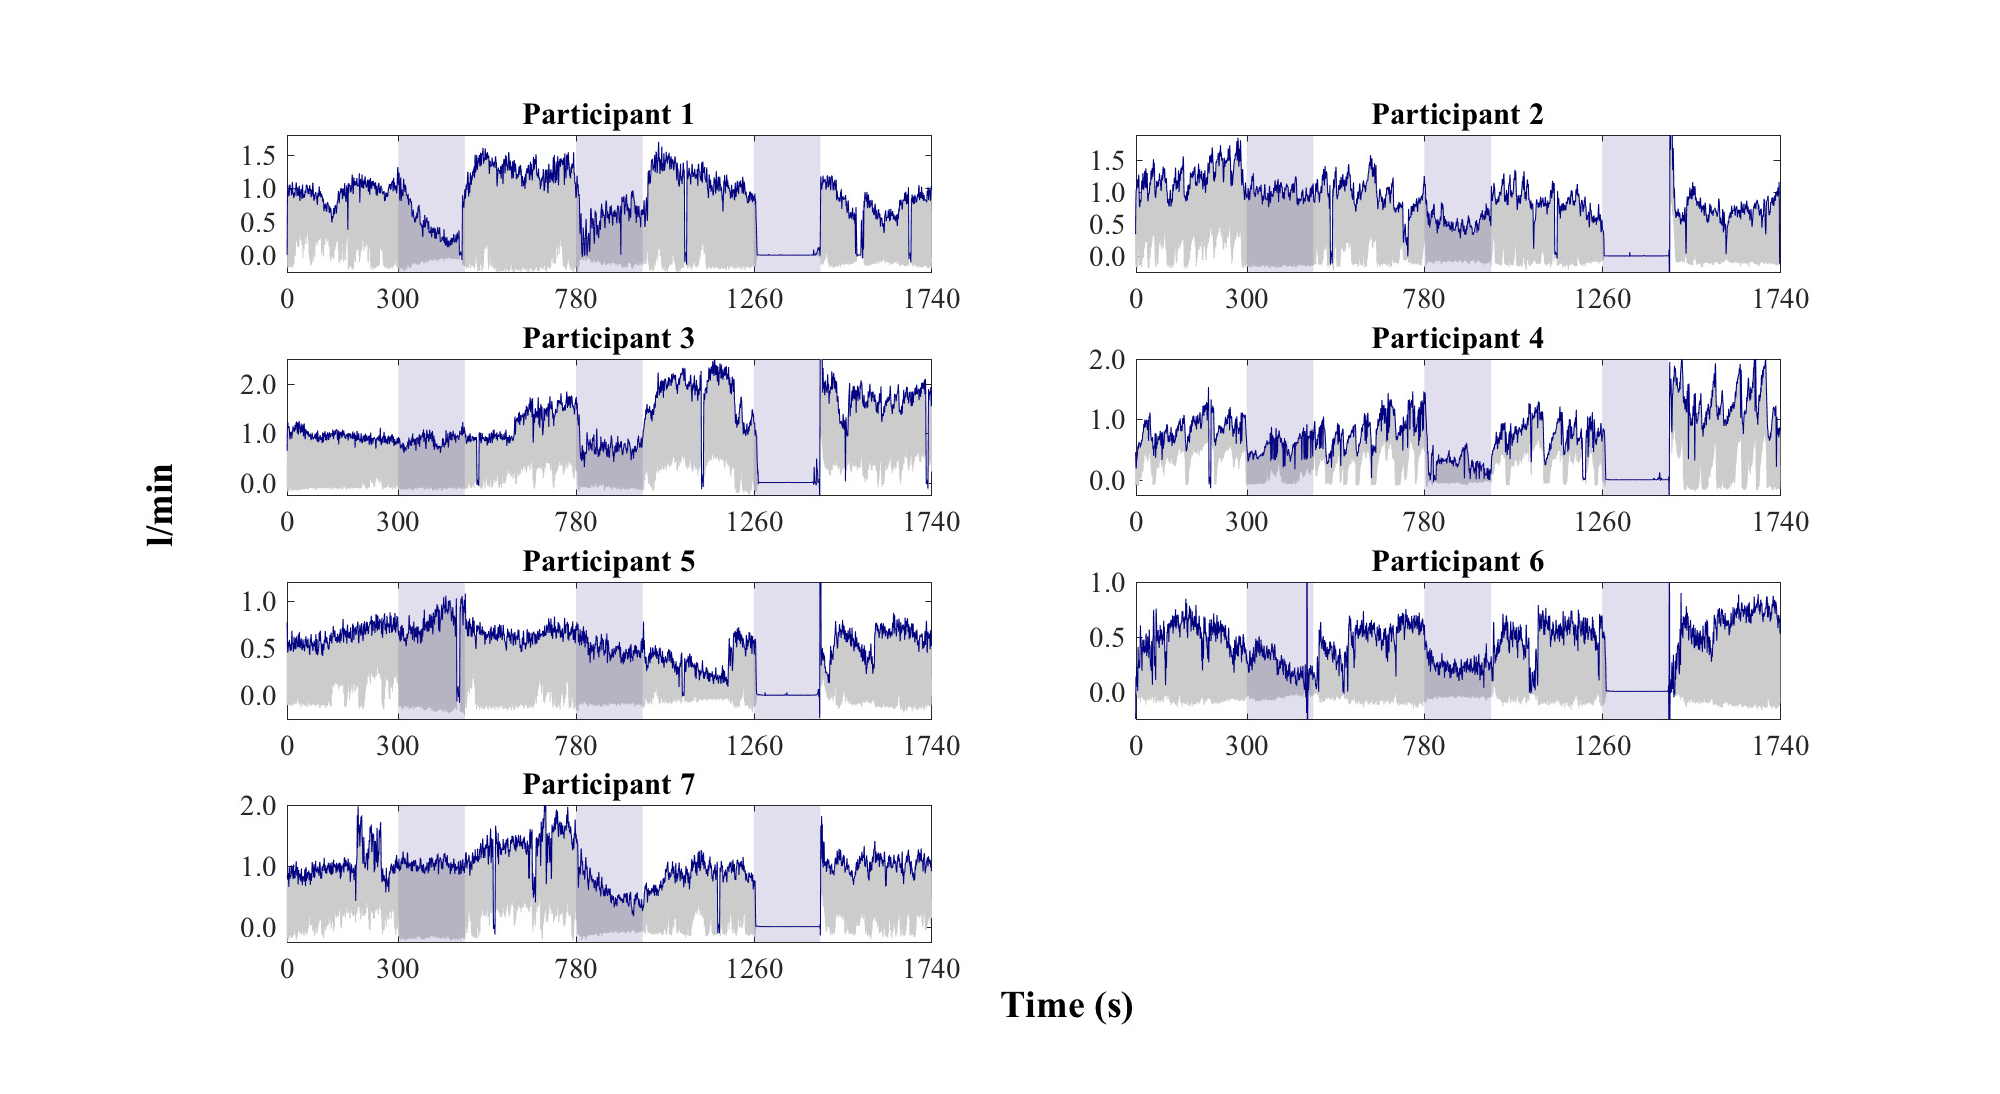
\includegraphics[width=\textwidth,height=\textheight,keepaspectratio,trim={2.5cm 0cm 2.5cm 0 cm},clip]{figure16}    
	\caption[Blood flow calculated from Doppler ultrasond device all along the whole expetiment]{Blood flow calculated from the Doppler ultrasound measurements for all the participants during the experiment. The grey out areas are the raw sign of the DU waveform. The dark blue lines represent the envelope calculated from the peak values. The blood flow was converted to the units (\si[per-mode=symbol]{\litre\per\minute}).}
	\label{fig:DU_flow}
\end{figure}

Figure \ref{fig:DU_flow} shows the peak values of the Doppler ultrasound converted into the blood flow. The shaded areas represent the occlusive events during the study. From a quantitative point of view, evidently, various participants showed a decline in their flow during venous occlusion in the region 2.  Participant 1 evidenced an exponential flow rate decrease during this part of the test. Moreover, participants 2 and 4 displayed a quick drop within the first seconds followed by a levelling at a mid-point. On the other hand, the rest of the participants did not show a significant change in flow rate during this transition. When the cuff's pressure was released only participants, 1 and 6 showed blood flow returning to the baseline value.  

During partial arterial occlusion, the change of arterial blood flow is unmistakable in most of the participants. Only, Participant 5 did not register a large shift in the circulatory flow. In contrast, all the participants showed a lack of signal during total occlusion. 

The numbers of the mean blood flow rate described in table \ref{tbl:DU_flow} are different from the ones shown in the figure. In general, in the transition from baseline to venous occlusion, most of the participants experience a drop of blood flow. The decline of the blood flow in region 2 was in average \SI{0.261(0134)}{\litre\per\min}. In contrast, participants 5 and 7 experienced a slight increase in the flow rate of approximately -0.055(0.062) l/min. After releasing the cuff's pressure, most participants showed an increase in their measured flow rate of about \SI{0.386(0231)}{\litre\per\min}. Participants 2 and  5 showed a decrease in their flow of \SIlist{-0.049;-0.084}{\litre\per\min}. 

\begin{table}[!htbp]
	\caption{Mean blood flow calculated form the plethysmography wave for baseline, total occlusion and return to normality}
	\label{tbl:DU_flow}
	\centering \small
	\begin{tabular}{lcccccccc}
		\toprule
		& \textbf{Region 1}
		& \textbf{Region 2}
		& \textbf{Region 3}
		& \textbf{Region 4}
		& \textbf{Region 5}
		& \textbf{Region 6}
		& \textbf{Region 7} \\
		& \textbf{[\si[per-mode=symbol]{\litre\per\minute}]}
		& \textbf{[\si[per-mode=symbol]{\litre\per\minute}]}
		& \textbf{[\si[per-mode=symbol]{\litre\per\minute}]}
		& \textbf{[\si[per-mode=symbol]{\litre\per\minute}]}
		& \textbf{[\si[per-mode=symbol]{\litre\per\minute}]}
		& \textbf{[\si[per-mode=symbol]{\litre\per\minute}]}
		& \textbf{[\si[per-mode=symbol]{\litre\per\minute}]} \\\midrule
		Participant 1    &     0.944     &     0.486     &     1.278     &     0.583     &     1.110     &     0.041     &     0.731     \\  
		Participant 2    &     1.245     &     1.003     &     0.954     &     0.551     &     0.841     &     0.013     &     0.760     \\  
		Participant 3    &     0.942     &     0.859     &     1.190     &     0.747     &     1.797     &     0.082     &     1.681     \\  
		Participant 4    &     0.823     &     0.543     &     0.817     &     0.305     &     0.755     &     0.040     &     1.266     \\  
		Participant 5    &     0.639     &     0.737     &     0.654     &     0.502     &     0.362     &     0.036     &     0.589     \\  
		Participant 6    &     0.496     &     0.256     &     0.477     &     0.240     &     0.499     &     0.029     &     0.600     \\  
		Participant 7    &     1.009     &     1.021     &     1.330     &     0.622     &     0.841     &     0.021     &     1.044     \\  
		\bottomrule
	\end{tabular}
\end{table}

During partial arterial occlusion, all the participants showed a decrease in their blood flow rate. In average, there was a reduction of \SI{-0.449(0212)}{\litre\per\min}. Which data is entirely in agreement with the partial restriction of their arterial blood flow. However, when the blood flow was restored from region 4 to 5 most of the partakers showed an increase in their blood flow. The increment of blood flow was in average \SI{0.466(0310)}{\litre\per\min}. The only one registering a decrease in the median was participant 5 which dropped \SI{0.141}{\litre\per\min}. 

During total occlusion event, all the participants showed an extreme decrease in their measured circulatory flow rate. As expected, no arterial or venous flow was recorded, the registered values might represent artefacts in the signals. After releasing the tourniquet, all the participants experience an increase in their flow rate to values of normality. 


%%********************************** % Section 5.7 ******************************************
\section{Measurements from Laser Doppler Flowmetry}
\label{section results 7}
The LDF device provided raw data in Volts which was converted into BPU units. This conversion was possible by applying equation \ref{eq:BPU} to the data collected.  As explained in section \ref{section:ldf}, the result produced is in arbitrary units which represent blood cells movement under the skin. Therefore, it illustrates the blood flow moving red blood cells in the micro-circulatory bed to distal parts of the tissue in the forearm.

The figure \ref{fig:LDF_flow} shows the peaks of the LDF waveform signal in BPU. A moving average was used to aggregate 20 seconds of data to the resultant plot. That plot shows the movement of the cell is affected when an occlusion occurs. It must be noticed that a noise artefact heavily impacted some parts of the data. Such as in participants 1 and 4.

\begin{figure}[!htb]
	\centering
	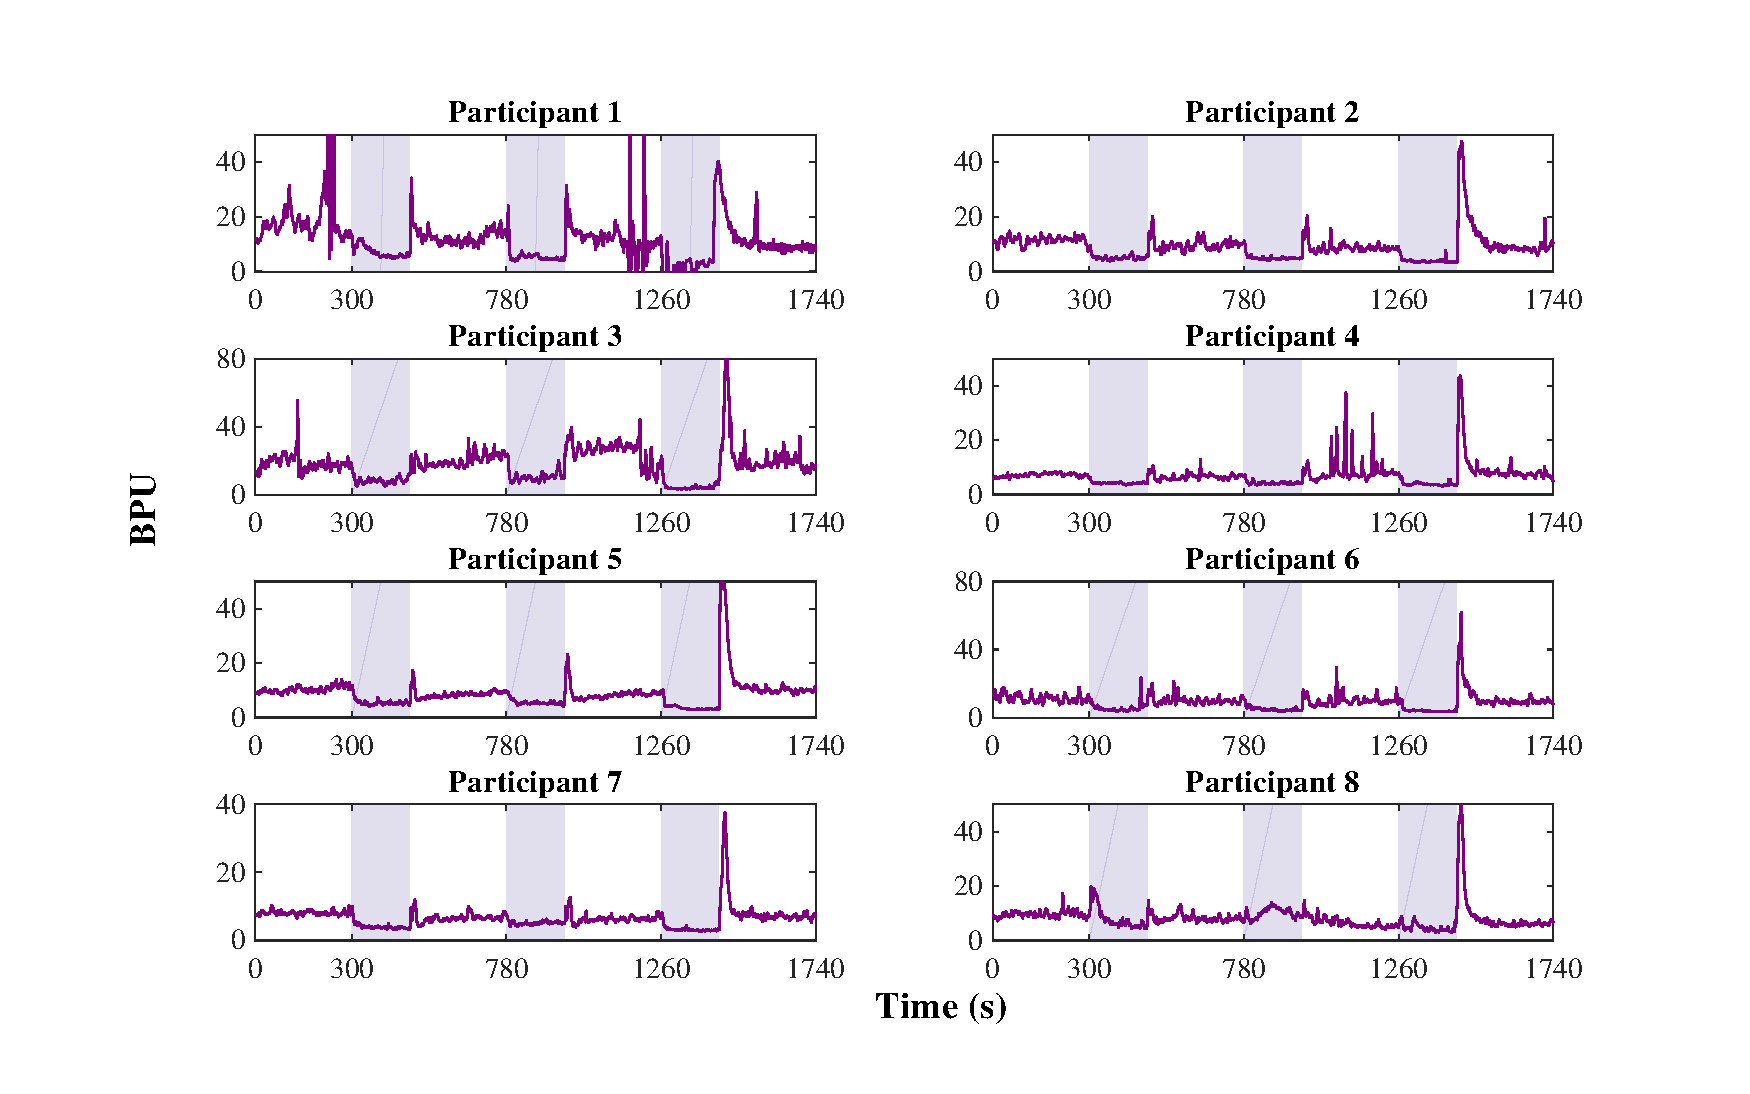
\includegraphics[width=\textwidth,height=\textheight,keepaspectratio,trim={2cm 0cm 2cm 0 cm},clip]{figure17}    
	\caption[Results of the LDF in BPU]{Results of the Laser Doppler Flowmetry measurement for all the participants after being converted to BPU. The values presented in purple are equivalent to envelope signal of the peak points.}
	\label{fig:LDF_flow}
\end{figure}

Nevertheless, a trend can be noticed in all the participants. During the occlusion in region 2, a slight decline in cell movement can be noticed. It shows that the venous occlusion slowed down the movement of RBC. After the cuff's pressure was released, a peak can be seen in most of the participants. This hyperaemic effect shows an acceleration of the RBC after the blockage event. 

Similar effects can be seen during partial arterial occlusion; the cells speed reduced compared to the previous baseline (region 3). Then as soon as the blockage was released, again the rush of RBCs can be detailed. Nevertheless, participant 8 seems to be an exception to the rule. His BPU tends to increase slightly during the transition of region 3 to 4. Moreover, contrary to the other signals in the transition from partial arterial occlusion to baseline in region 5, his BPU decreased. This results also could explain some of the adverse readings captured by the iPG signals.

Lastly, during total occlusion, all the mean BPUs of the participants reduced considerably. Then later when the tourniquet was released, the rush of blood flow can be noticed in the hyperaemic effect registered by the instrument, which was also detected by others instruments.

Table \ref{tbl:LDF_flow} reviews the values of the mean BPU data obtained. The results declared there are in complete agreement with the figure previously analysed.

\begin{table}[!htbp]
	\caption{Mean blood flow calculated form the plethysmography wave for baseline, total occlusion and return to normality}
	\label{tbl:LDF_flow}
	\centering \small
	\begin{tabular}{lcccccccc}
		\toprule
		& \textbf{Region 1}
		& \textbf{Region 2}
		& \textbf{Region 3}
		& \textbf{Region 4}
		& \textbf{Region 5}
		& \textbf{Region 6}
		& \textbf{Region 7} \\
		& \textbf{[BPU]}
		& \textbf{[BPU]}
		& \textbf{[BPU]}		
		& \textbf{[BPU]}		
		& \textbf{[BPU]}
		& \textbf{[BPU]}
		& \textbf{[BPU]}\\\midrule
		Participant 1    &     42.89     &     12.71     &     18.37     &      9.52     &     36.44     &     11.75     &     19.64     \\  
		Participant 2    &     17.05     &      9.18     &     15.24     &      8.32     &     14.38     &      6.46     &     21.22     \\  
		Participant 3    &     30.69     &     17.08     &     33.42     &     20.72     &     40.28     &      9.27     &     38.08     \\  
		Participant 4    &     10.14     &      6.27     &     10.61     &      7.18     &     16.22     &      6.67     &     15.73     \\  
		Participant 5    &     16.66     &     10.49     &     14.16     &      9.56     &     14.58     &      5.73     &     23.70     \\  
		Participant 6    &     19.82     &     11.41     &     18.43     &      9.75     &     17.87     &      7.83     &     19.14     \\  
		Participant 7    &     12.54     &      7.45     &     11.08     &      9.32     &     10.96     &      5.91     &     14.83     \\  
		Participant 8    &     15.76     &     13.54     &     14.36     &     17.74     &     12.33     &      9.21     &     16.08     \\  
 		\bottomrule
\end{tabular}
\end{table}



%%********************************** % Section 5.8 ******************************************
\section{Measurements Red-light from PPG signal}
\label{section results 8}
The PPG device provides information about the change of volume within the vascular bed under the skin. It is capable of detecting either venous or arterial blood change according to the light wavelength being used \mynote{check if this is true or find a reference}. The device employed in the experiment has an output port which provides the unprocessed raw photoplethysmography waveform. Similarly, as in the iPG signal, the PPG is composed of DC and AC parts. The DC portion of the signal is equivalent to the blood volume under the light beam. It also contains data about respiratory rate and other physiological information. On the other hand, the AC component changes in amplitude synchronously according to the cardiac cycle and blood volume in the capillaries. 

During the experiment performed changes in DC and AC components can be easily identified as showed in figure \ref{fig:RED_PPG}. In the plot, the shaded regions represent each occlusive event during the test. On the left, it is illustrated the DC component of the PPG per each participant. This signal was obtained by detecting the low envelope values of the raw PPG waveform. In other words, the points on the foot of the waveform.  On the right-hand side is the AC component of the signal obtained by removing the low envelope of the raw data. Next, the waveform was inverted to leave only the dynamic element of the signal. Last, the peaks detected from the plethysmography waveform were redrawn in black highlighting the maximum values during all the occlusive events.  

\begin{figure}[!htbp]
	\centering
	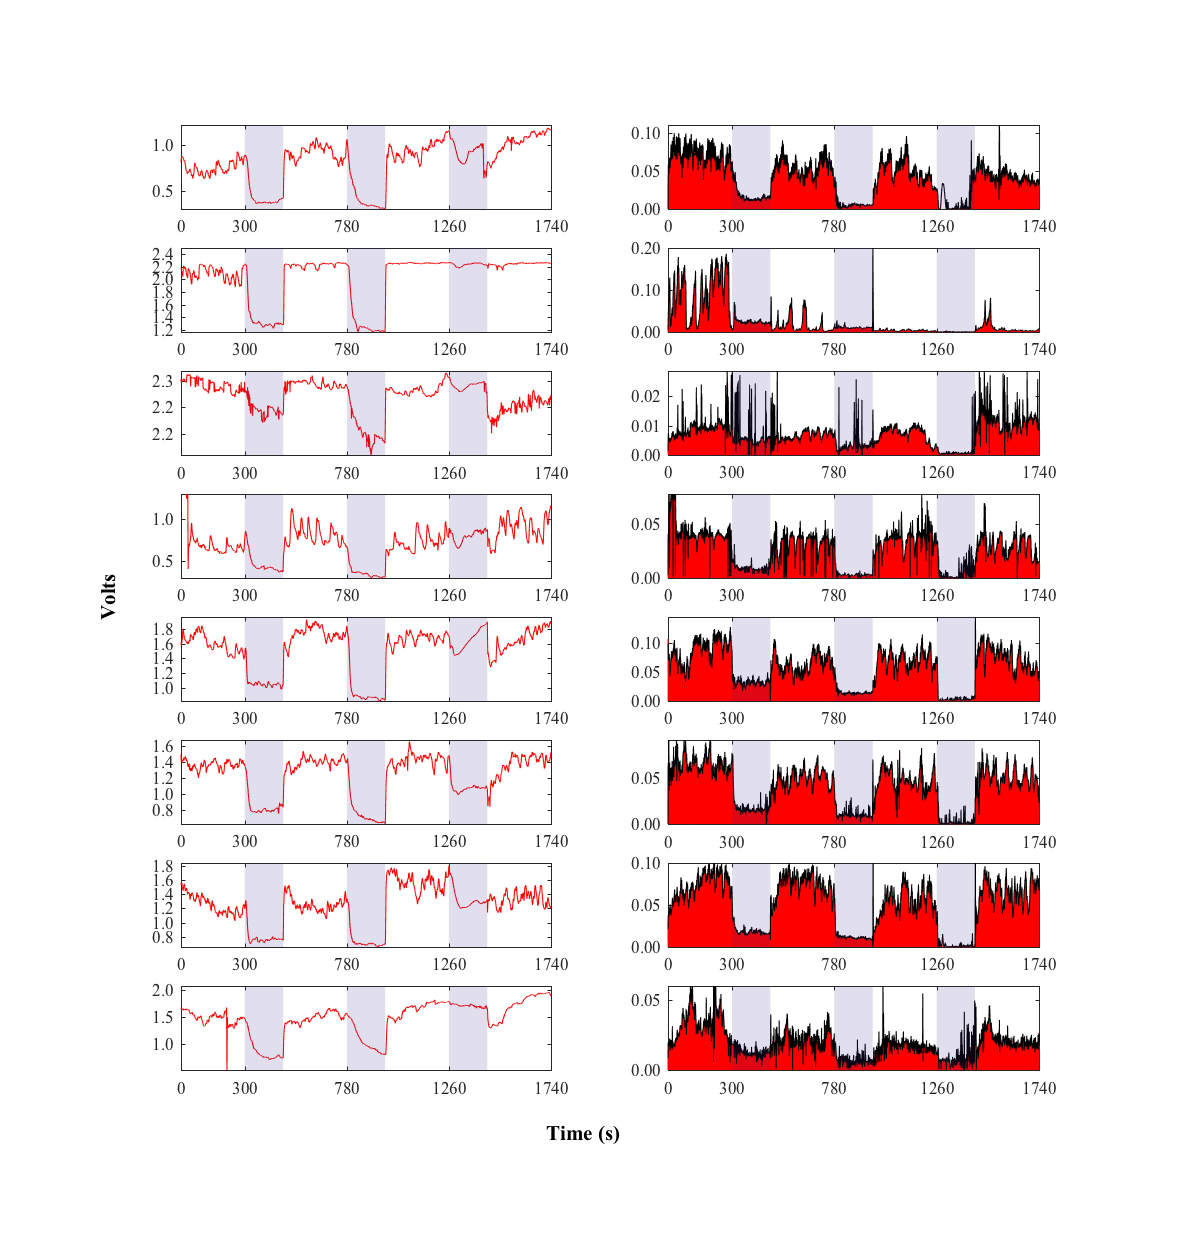
\includegraphics[width=\textwidth,keepaspectratio,trim={1cm 0cm 0cm 0 cm},clip]{figure18}    
	\caption[PPG red wavelength measurments AC and DC components]{Measurements from the red wavelength PPG sensor. On the left, the DC component of the signal, it only includes the lower envelope of the waveform. On the right, the AC component of the red wavelength where the foot of the signal has been aligned to zero. The envelope showed in black describes the peaks of the signal}
	\label{fig:RED_PPG}
\end{figure}

\begin{table}[!htbp]
	\caption[Mean peak value of the PPG DC signal for all participants in all regions]{Mean peak value of the PPG DC signal for all the participants in all the regions.}
	\label{tbl:PPG RED DC}
	\centering \small
	\begin{tabular}{lcccccccc}
		\toprule
		& \textbf{Region 1}
		& \textbf{Region 2}
		& \textbf{Region 3}
		& \textbf{Region 4}
		& \textbf{Region 5}
		& \textbf{Region 6}
		& \textbf{Region 7} \\
		& \textbf{[\si{\volt}]}
		& \textbf{[\si{\volt}]}
		& \textbf{[\si{\volt}]}		
		& \textbf{[\si{\volt}]}		
		& \textbf{[\si{\volt}]}
		& \textbf{[\si{\volt}]}
		& \textbf{[\si{\volt}]}\\\midrule
		Participant 1    &     0.75      &     0.44      &     0.91      &     0.43      &     0.94      &     0.91      &     1.03      \\  
		Participant 2    &     2.09      &     1.38      &     2.22      &     1.33      &     2.25      &     2.24      &     2.24      \\  
		Participant 3    &     2.24      &     2.20      &     2.24      &     2.16      &     2.23      &     2.24      &     2.20      \\  
		Participant 4    &     0.76      &     0.46      &     0.80      &     0.36      &     0.72      &     0.79      &     0.89      \\  
		Participant 5    &     1.60      &     1.07      &     1.73      &     0.93      &     1.66      &     1.64      &     1.64      \\  
		Participant 6    &     1.36      &     0.84      &     1.38      &     0.76      &     1.41      &     1.08      &     1.35      \\  
		Participant 7    &     1.26      &     0.79      &     1.25      &     0.75      &     1.56      &     1.32      &     1.34      \\  
		Participant 8    &     1.48      &     0.88      &     1.48      &     1.07      &     1.64      &     1.71      &     1.70      \\  
		\bottomrule
	\end{tabular}
\end{table}

From the DC signal point of view, all the participants showed a clear drop in their DC components of the signal during venous occlusion (region 2) and partial arterial occlusion (region 4). It can be seen from the figure, that the DC value dropped dramatically in most participants after the occlusive event. Nevertheless, Participant 3 showed an exponential decrease in his recorded readings. Effectively, this changes can be clearly confirmed when analysing the mean values of the DC data described in Table \ref{tbl:PPG RED DC}. From there, it is calculated that the average baseline before the occlusions were \SI{1.44(055)}{\volt} for Region 1 and \SI{1.51(054)}{\volt} for Region 3. During the occlusive transitions, the DC components dropped about \SI{-0.435(0210)}{\milli\volt} and \SI{-0.528(0247)}{\milli\volt} for region 2 and region 4 respectively. Nevertheless, during total occlusion, the signals obtained were erratic with no clear shape or direction. Some participants showed a slight decrease, but others did not exhibit significant changes. In general, DC data provided valuable information during the venous and partial arterial occlusion but not conclusive result during total blood flow stoppage. 

\begin{table}[!htbp]
	\caption[Mean peak value of the PPG AC signal for all participants in all regions]{Mean peak value of the PPG AC signal for all the participants in all the regions.}
	\label{tbl:PPG RED AC}
	\centering \small
	\begin{tabular}{lcccccccc}
		\toprule
		& \textbf{Region 1}
		& \textbf{Region 2}
		& \textbf{Region 3}
		& \textbf{Region 4}
		& \textbf{Region 5}
		& \textbf{Region 6}
		& \textbf{Region 7} \\
		& \textbf{[\si{\milli\volt}]}
		& \textbf{[\si{\milli\volt}]}
		& \textbf{[\si{\milli\volt}]}		
		& \textbf{[\si{\milli\volt}]}		
		& \textbf{[\si{\milli\volt}]}
		& \textbf{[\si{\milli\volt}]}
		& \textbf{[\si{\milli\volt}]}\\\midrule
		Participant 1    &     724.83    &     180.45    &     546.76    &      66.13    &     490.87    &     109.85    &     441.54    \\  
		Participant 2    &     926.02    &     245.24    &     158.34    &     110.32    &      51.30    &       5.97    &      92.58    \\  
		Participant 3    &      94.21    &      69.72    &      68.76    &      37.19    &      71.62    &      10.54    &     122.67    \\  
		Participant 4    &     436.74    &      92.42    &     315.26    &      37.22    &     354.44    &      58.08    &     296.36    \\  
		Participant 5    &     873.38    &     324.60    &     638.53    &     155.21    &     703.81    &      51.36    &     751.62    \\  
		Participant 6    &     658.05    &     188.75    &     501.10    &     112.57    &     480.41    &      38.14    &     517.01    \\  
		Participant 7    &     731.50    &     190.43    &     746.34    &     125.76    &     547.89    &      26.92    &     660.43    \\  
		Participant 8    &     360.69    &     130.06    &     216.80    &      74.43    &     168.52    &      89.77    &     217.06    \\ 
		\bottomrule
	\end{tabular}
\end{table}

On the other hand, AC component produced distinctive results during each blockage event. In comparison with the DC, the AC signal was able to detect changes during total occlusion which is concurrent with the fact that there is no change of volume at that moment. Reviewing the AC signals qualitatively seemingly participant 2 registered noisy waveforms during the region 1 of the study. Also, Participant 3 had noisy peaks during the whole test, but changes through each occlusion are still visible

From the numeric point of view, Table \ref{tbl:PPG RED AC} shows the average values of the amplitude in mV. During baseline, the mean peak value was \SI{600.67(28201)}{\milli\volt}, \SI{398.98(24421)}{\milli\volt}, \SI{358.61(23913)}{\milli\volt} and \SI{387.4073(24531)}{\milli\volt} for regions 1,3,5 and 7 respectively. In general, during venous occlusion, the signal amplitude decreased in all participants about \SI{-422.97(21217)}{\milli\volt}. Participant 5 had the smallest change (\SI{-24.50}{\milli\volt}) compared to the rest of the signals. 

After the cuff's pressure had been relieved during the transition from venous occlusion to baseline, participants 2 and 3 showed an increase of their mean amplitude. The rest displayed a recovery in their signal peak to peak of approximately \SI{221.28(21124)}{\milli\volt}. Then, during partial arterial occlusion, all participants showed a decreased in their mean PPG signals amplitude in average \SI{-309.14(21943)}{\milli\volt}. When comparing mean values during occlusions in region 2 and 4, the signal amplitude in region 4 was slightly lower than the one in region 2 by about \SI{-87.86(4691)}{\milli\volt}. 

Lastly, during total occlusion, all the participants demonstrated a substantial decrease in their AC amplitudes. All in all, signals went below 109 mv with an average value of \SI{-48.83(3662)}{\milli\volt}.

In conclusion, PPG waveform experienced changes of DC and AC components during each type of occlusion through the study. The DC signal was able to detect changes during venous and partial arterial occlusions. The difference in mean values of these two events was minimum. Nevertheless, the DC component did not show significant changes during total occlusion.  On the other hand, the AC component was able to detect changes during all occlusions, being each mean peak value significantly lowers during each test. 

%%********************************** % Section 5.9 ******************************************
\section{Measurements from the ECG device}
\label{section results 9}
The ECG signals collected provide details of the electrical activity of the heart during the whole study. Hence, no changes were registered through the test unless a bad connection occurs. The data gathered works as a clock reference during the data processing. Also, it helps as a reference to calculate pulse transit time with the other dynamic signals obtained. \mynote{Check if I am going to publish measurements about PTT. If not this paragraph should be modified}. Figure \ref{fig:ECG} shows the typical ECG for one of the participants.

\begin{figure}[!htbp]
	\centering
	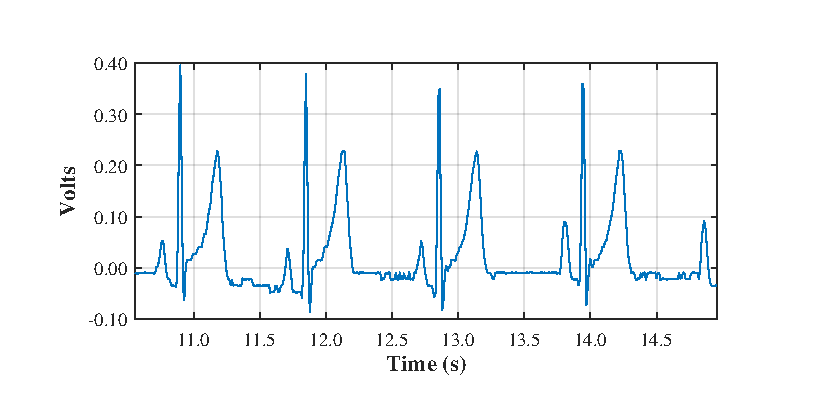
\includegraphics{figure19}    
	\caption[ECG measurement acquired by the system]{Measurement from one of the participants. Clearly, it can be identified the points P, Q, R, S and T. This signal did not change during the whole experiment.}
	\label{fig:ECG}
\end{figure} 

All the waveforms detected were normal and provided enough information about the characteristic peaks in an ECG waveform. The points P, Q, R, S and T are clearly visible in all the signals. Nonetheless, Participant 1 showed an elevated T wave due to his athletic career. According to him, he had a ventricular hypertrophy where one of his ventricles was enlarged.  

%%********************************** % Section 5.10 ******************************************
\section{Conclusions}
\label{section results 10}
All the signals recorded were clear and offered an overview of what could happen during each occlusive event. It was demonstrated, that the designed impedance device was able to detect changes in basal impedance and plethysmography signals. Moreover, it seems that each occlusive event manifests a particular response like slope change in basal impedance and waveform amplitude at systolic and diastolic peaks during occlusions. 

The other instruments were also able to detect changes during each event. For instance, the ultrasound device, referencing arterial flow, detected changes mostly in region 4 and 6 of the study. The LDF pointing towards microcirculatory flow was able to detect variations in flow in all the events. Moreover, it showed special sensitivity as soon as the flow was restored showing. A clear hyperaemic response of the capillaries was portrayed in the signals. Lastly, red wavelength PPG was able to detect changes during all the events. The DC component of the signal detected changes during venous occlusion and partial arterial occlusion but in total blockage did not show a clear response. On the other hand, AC component showed variations to all occlusions showing sharp changes in amplitude during each occlusive episode. 